\documentclass[aspectratio=169]{beamer}
\usepackage{will_handley_beamer}
\usepackage{title_page}

% Commands
% --------
% - \arxiv{arxiv number}
% - \arxiv{<number>}            arxiv.org/abs/<number>
% - \oldarxiv{<arxiv number>}   arxiv.org/<number>
% - \doi{<doi>}                 doi.org/<doi>
% - \xkcd{<number>}             xkcd.com/<number>
% - \email{<email>}             <<email>>
% - \tthref{<website>}          <website>
% - \av[dist]{<quantity>}       <quantity>_{dist}
% - \student{<name>}{<detail>}{<photo>}

% Talk details
% ------------
\title{Cosmic Tensions}
\subtitle{A High Energy Physicist's Primer}
\date{31\textsuperscript{st} January 2025}

\begin{document}

\begin{frame}
    \titlepage
\end{frame}

\begin{frame}
    \frametitle{Introduction: Precision Cosmology and its Discontents}
    \vspace{-0.1cm}
    \begin{columns}
        \column{0.5\textwidth}
        \begin{itemize}
            \item Have well-and-truly entered an era of precision cosmology.
            \item Multiple independent observations allow us to constrain the parameters of our cosmological model.
            \item The Standard Model of Cosmology ($\Lambda$CDM) successfully explains a wide range of observations.
            \item However, increasing precision has revealed inconsistencies, or tensions, between different measurements.
            \item Are these tensions cracks in $\Lambda$CDM, hints of new physics, or simply measurement systematics?
        \end{itemize}
        \column{0.5\textwidth}
        \includegraphics[width=\textwidth]{figures/cosmos.png}
    \end{columns}
\end{frame}

%COMPACT:2022gbl 2210.11426
%SPT-3G:2021wgf 2103.13618
%Pan:2023mie 2310.07260
%Pandya:2024jqg 2408.00726
%Saraf:2024log 2406.02857
%Sorrenti:2024ugq 2407.07002
%Zurek:2024qfm 2401.03025
%Abghari:2024eja 2405.09762
%Anchordoqui:2024gfa 2404.17334
%Bargiacchi:2023jse 2303.07076
%Bousis:2024rnb 2405.07039
%Dimastrogiovanni:2024xvc 2403.13581
%G:2019dar 1909.06391
%Huang:2024erq 2401.14170
%Iosifidis:2024ksa 2406.01412
%Bird:2008hn 0807.4933
%DESI:2018ymu 1804.08657
%Feldman:2009es 0911.5516
%Watkins:2008hf 0809.4041
%Park:2018tgj 1809.03598
%Park:2017xbl 1801.00213
%Vagnozzi:2020rcz 2010.02230
%Vagnozzi:2020dfn 2011.11645
%Efstathiou:2020wem 2002.06892
%Handley:2019tkm 1908.09139
%DiValentino:2019qzk 1911.02087
%Chluba:2023xqj 2309.12083
%Wang:2024hen 2405.03368
%Zuniga:2024wau 2405.13280
%Handley:2019wlz 1902.04029
%Glanville:2022xes 2205.05892
%Chen:2024tfp 2402.14070
%Castello:2024jmq 2404.09379
%Akarsu:2024eoo 2406.07526
%Liu:2023xtb 2312.15760
%Lynch:2024hzh 2406.10202
%Qiao:2024ehj 2403.05682
%Sunayama:2023hfm 2309.13025
%vonHausegger:2024jan 2404.07929
%Euclid:2024wly 2401.17945
%Koblischke:2024hft 2406.19375
%Gomez-Vargas:2024izm 2405.03293
%Gomez-Valent:2024tdb 2404.18845
%Giare:2024gpk 2407.16689
%Frion:2023xwq 2307.06320
%Favale:2024lgp 2402.13115
%deSouza:2024sfl 2403.04970
%Capozziello:2020dvd 2004.11557
%DESI:2024aqx 2405.04216
%Asghari:2024obf 2405.11840
%Kuo:2012hg 1207.7273
%Kristian:1965sz None
%Friedman:1922kd None
%Huang:2018dbn 1801.02711
%Whitelock:2012yk 1210.7307
%Huang:2024exg 2401.09581
%Rizzi:2007ni astro-ph/0701518
%Freedman:2021ahq 2106.15656
%Pietrzynski:2019cuz None
%Gaia:2016zol 1609.04153
%Celerier:2024dvs 2407.04452
%SPT-3G:2024qkd 2403.17925
%McVittie:1933zz None
%Jovanovic:2023tcc 2305.13448
%Jovanovic:2022twh 2211.12951
%Zakharov:2016lzv 1605.00913
%DiValentino:2018gcu None
%Piffaretti:2010my 1007.1916
%Voges:1999ju astro-ph/9909315
%Borgani:1999ek astro-ph/9901017
%SPT:2016izt 1603.06522
%Borgani:2001ir astro-ph/0106428
%Bohringer:2007vs astro-ph/0703553
%Reiprich:2001zv astro-ph/0111285
%Schellenberger:2017wdw 1705.05842
%Toomet:1999yw astro-ph/9907238
%Mroczkowski:2018nrv 1811.02310
%Sunyaev:1972eq None
%MAGIC:2019ozu 1904.00134
%Fermi-LAT:2018lqt 1812.01031
%Fialkov:2019vnb 1902.02438
%Ponente:2011se 1104.3012
%Fermi-LAT:2015otn 1511.00693
%Cappelluti:2017miu 1702.01660
%Gilmore:2009zb 0905.1144
%Einasto:2011zc 1105.2124
%Sekiguchi:2020teg 2007.03381
%Hart:2021kad 2107.12465
%Lee:2022gzh 2212.04494
%Hoshiya:2022ady 2202.07714
%Madore:2023voh 2311.05048
%Bekenstein:1982eu None
%Damour:1994zq hep-th/9401069
%Hauser:2001xs astro-ph/0105539
%Umetsu:2020wlf 2007.00506
%Dhawan:2017ywl 1707.00715
%Galbany:2022zir 2209.02546
%Jones:2022mvo 2201.07801
%Uzan:2002vq hep-ph/0205340
%Uzan:2010pm 1009.5514
%Martins:2017yxk 1709.02923
%Martins:2015dqa 1503.05068
%Kaplinghat:1998ry astro-ph/9810133
%Avelino:2000ea astro-ph/0008446
%Battye:2000ds astro-ph/0008265
%Avelino:2001nr astro-ph/0102144
%Rocha:2003gc astro-ph/0309211
%Martins:2003pe astro-ph/0302295
%Scoccola:2009xtv 0910.1083
%Menegoni:2012tq 1202.1476
%Goobar:2016uuf 1611.00014
%Goobar:2022wan 2211.00656
%Rodney:2021keu 2106.08935
%Pierel:2024frl 2404.02139
%Pierel:2024rjr 2403.18954
%Birrer:2022chj 2210.10833
%Suyu:2023jue 2301.07729
%Treu:2022aqp 2210.15794
%Suyu:2018vqs 1801.07262
%Humphreys:2007ir 0709.0925
%Bragg:2000in astro-ph/0001543
%Reid:2012hm 1207.7292
%Braatz:2010sg 1005.1955
%Reid:2008nm 0811.4345
%Gao:2015tqd 1511.08311
%Kuo:2014bqa 1411.5106
%Kuo:2010uy 1008.2146
%Herrnstein:1999kd astro-ph/9907013
%Freedman:2019jwv 1907.05922
%Perivolaropoulos:2014lua 1401.5044
%Bertolami:2020ldj 2002.08184
%Boylan-Kolchin:2021fvy 2103.15825
%Lee:2020lof 2008.02583
%Aurich:2004fq astro-ph/0412569
%Alnes:2005nq astro-ph/0506449
%Liang:2022smf 2211.02473
%Artis:2024eco 2402.08459
%Milgrom:1983ca None
%Dainotti:2008vw 0809.1389
%Anand:2024nim 2401.04776
%Lee:2023vku 2312.02282
%Li:2024yoe 2401.04777
%Huang:2019yhh 1908.10883
%Huang:2023frr 2312.08423
%Blakeslee:2021rqi 2101.02221
%Anand:2024lbl 2405.03743
%deJaeger:2022lit 2203.08974
%Csornyei:2023rpw 2302.03112
%Kourkchi:2022ifq 2201.13023
%Riess:2024vfa 2408.11770
%HST:2000azd astro-ph/0012376
%Reid:2019tiq 1908.05625
%Scolnic:2021amr 2112.03863
%Brout:2022vxf 2202.04077
%Riess:2021jrx 2112.04510
%Breuval:2024lsv 2404.08038
%Zhevakin:1963dz None
%Leavitt:1912zz None
%Hoffmann:2016nvl 1607.08658
%Breuval:2023rkw 2304.00037
%Riess:2019cxk 1903.07603
%Riess:2023bfx 2307.15806
%Riess:2024ohe 2401.04773
%Kennicutt:1997dm astro-ph/9712055
%Sakai:2004ys astro-ph/0402499
%Macri:2006wm astro-ph/0608211
%Bhardwaj:2023mau 2309.03263
%Anderson:2016txx 1604.05691
%Romaniello:2021vht 2110.08860
%Zaritsky:1994ht None
%Riess:2005zi astro-ph/0503159
%Riess:2009pv 0905.0697
%Galbany:2016cqf 1603.07808
%Mochejska:1999nd astro-ph/9908293
%Follin:2017ljs 1707.01175
%Perivolaropoulos:2021bds 2109.04406
%Benedict:2006cp astro-ph/0612465
%Casertano:2015dso 1512.09371
%Riess:2018uxu 1801.01120
%Riess:2020fzl 2012.08534
%Li:2022aho 2202.11110
%Anderson:2012dv 1212.5119
%Breuval:2020trd 2006.08763
%Riess:2022mme 2208.01045
%Reyes:2022boz 2208.09403
%Li:2021qkc 2107.08029
%Argon:2004re astro-ph/0407486
%Bonanos:2006jd astro-ph/0606279
%Bresolin:2009bv 0905.2791
%Ngeow:2005qc astro-ph/0507601
%Sandage:2008rq 0810.1780
%Kodric:2013pz 1301.6170
%Kushnir:2024spm 2404.16102
%Argon:2007ry astro-ph/0701396
%Kormendy:2013dxa 1304.7762
%Pesce:2015tga 1507.07904
%Pesce:2020xfe 2001.09213
%Lee:1993jb None
%Li:2024gib 2403.17048
%Jensen:2021ooi 2105.08299
%Wu:2022hxf 2211.06354
%Anderson:2023aga 2303.04790
%2017ApJ...845..146H 1703.06468
%2000ApJ...542..804N astro-ph/0003012
%Madore:2020yqv 2005.10792
%1997MNRAS.289..406S astro-ph/9703186
%2002PASP..114..375S astro-ph/0201387
%Farag:2023xid 2310.13142
%Saltas:2022aua 2203.02499
%2007ApJ...661..815R astro-ph/0701518
%Anand:2021sum 2108.00007
%Li:2023pmo 2304.06695
%Soltis:2020gpl 2012.09196
%1998ApJ...500..525S astro-ph/9710327
%2011ApJ...737..103S 1012.4804
%Anderson:2021fsp 2108.09067
%Scolnic:2023mrv 2304.06693
%2002AJ....124..213M astro-ph/0204192
%2006AJ....132.2729M astro-ph/0603073
%2009ApJ...690..389M 0809.2598
%Beaton:2018fyo 1808.09191
%Csornyei:2023enu 2305.13943
%Euclid:2024yrr 2405.13491
%Newman:2024fkx 2406.03532
%2004MNRAS.351.1204V astro-ph/0403563
%2012ApJS..198....6D 1109.6893
%2014AJ....148....7W 1404.2987
%2018ApJ...858...11M 1803.01278
%2018ApJ...858...12H 1803.01277
%Lee:2022akw 2205.11323
%SNLS:2007cqk astro-ph/0701828
%Kenworthy:2021azy 2104.07795
%Burns:2010ka 1010.4040
%2011ApJ...731..120M 1011.5910
%SNLS:2011lii 1104.1443
%Dhawan:2020xmp 2001.09260
%Murakami:2023xuy 2306.00070
%Peterson:2021hel 2110.03487
%Brownsberger:2021uue 2110.03486
%Jones:2018vbn 1805.05911
%CSP:2018rag 1809.06381
%Garnavich:2022hef 2204.12060
%Dhawan:2022yws 2203.04241
%Dhawan:2022gac 2211.07657
%Carr:2021lcj 2112.01471
%Popovic:2021yuo 2112.04456
%2015ApJ...802...20R 1412.6501
%Riess:2011yx 1103.2976
%Wojtak:2024mgg 2403.10388
%Khetan:2020hmh 2008.07754
%DES:2018rjw 1811.02376
%Feeney:2018mkj 1802.03404
%Freedman:2024eph 2408.06153
%Freedman:2020mho 2005.10793
%Lee:2023zsq 2305.02453
%2015AJ....149..117M 1412.1511
%Parada:2020rpk 2011.11681
%Lee:2024qzr 2408.03474
%Parada:2023wyt 2303.16934
%Li:2023utj 2306.10103
%Smartt:2009zr 0908.0700
%Kilpatrick:2023pse 2306.04722
%1974ApJ...193...27K None
%Baron:2004wb astro-ph/0410153
%Dessart:2005gg astro-ph/0505465
%Hamuy:2002tj astro-ph/0201279
%Gall:2017gva 1705.10806
%Dessart:2005ax astro-ph/0504028
%Vogl:2018ckb 1811.02543
%Jones:2008tz 0810.5538
%Gall:2016qvq 1603.04730
%Dhungana:2023dep 2308.00916
%Dessart:2007rt 0711.1815
%Vogl:2019fhc 1911.04444
%deJaeger:2020zpb 2006.03412
%Hamuy:2002qx astro-ph/0209174
%SNLS:2006mwe astro-ph/0603535
%deJaeger:2023vkm 2305.17243
%Bose:2014sza 1401.5115
%Blakeslee:2009tc 0901.1138
%Moresco:2022phi 2201.07241
%Cantiello:2023obe 2307.03116
%Tonry:2000aa astro-ph/0011223
%2009ApJ...700.1247R 0907.1408
%Sales:2022ich 2206.05295
%Planck:2018vyg 1807.06209
%Raimondo:2009qs 0907.1408
%WST:2024rai 2403.05398
%Jimenez:2001gg astro-ph/0106145
%Simon:2004tf astro-ph/0412269
%Stern:2009ep 0907.3149
%Moresco:2015cya 1503.01116
%Moresco:2016mzx 1601.01701
%Ratsimbazafy:2017vga 1702.00418
%Borghi:2021zsr 2106.14894
%Jiao:2022aep 2205.05701
%Tomasetti:2023kek 2305.16387
%Jimenez:2023flo 2306.11425
%Moresco:2023zys 2307.09501
%Busti:2014dua 1402.5429
%Cao:2017ivt 1708.08635
%Yu:2017iju 1711.03437
%Gomez-Valent:2018hwc 1802.01505
%Haridasu:2018gqm 1805.03595
%Gomez-Valent:2021hda 2111.15450
%Bonilla:2020wbn 2011.07140
%OColgain:2021pyh 2101.08565
%Liu:2022lqw 2204.07365
%Yang:2022jkf 2204.01020
%Favale:2023lnp 2301.09591
%Yang:2024epu 2401.03413
%Rani:2016wff 1612.07492
%Li:2015nta 1504.03269
%Capozziello:2020ctn 2003.09341
%Moresco:2012by 1201.6658
%Moresco:2016nqq 1604.00183
%EUCLID:2011zbd 1110.3193
%LSST:2008ijt 0805.2366
%Heavens:2014rja 1409.6217
%Verde:2016ccp 1607.05297
%Amati:2018tso 1811.08934
%Wei:2019uss 1912.00668
%Sahni:2014ooa 1406.2209
%Zheng:2016jlq 1604.07910
%Zheng:2018sxp 1803.09106
%2000A&ARv..10....1K astro-ph/9911094
%Chavez:2014ria 1405.4010
%2011ApJ...735...52B 1104.4719
%2011MNRAS.416.2981P 1106.4558
%2016MNRAS.462.2431C 1607.06458
%Gonzalez-Moran:2019uij 1906.02195
%Chavez:2024twa 2404.16261
%Gardner:2006ky astro-ph/0606175
%2008MNRAS.384..449F 0704.3704
%2009MNRAS.398.1601F 0809.3437
%Feroz:2013hea 1306.2144
%Ratra:1987rm None
%Wetterich:1987fm 1711.03844
%Chevallier:2000qy gr-qc/0009008
%Linder:2002et astro-ph/0208512
%2003RvMP...75..559P astro-ph/0207347
%FernandezArenas:2017dux 1710.05951
%1964MNRAS.128..307R None
%Treu:2016ljm 1605.05333
%XXX:2014xxi 1404.6014
%Kelly:2014mwa 1411.6009
%Kelly:2023mgv 2305.06367
%Grillo:2024rhi 2401.10980
%Jee:2015yra 1509.03310
%Linder:2011dr 1109.2592
%Suyu:2013kha 1306.4732
%Collett:2019hrr 1905.09781
%Pierel:2020tav 2010.12399
%DES:2019fny 1910.06306
%Millon:2019slk 1912.08027
%Wagner:2018rae 1809.03505
%Birrer:2020tax 2007.02941
%Birrer:2020jyr 2008.06157
%Oguri:2010ns 1001.2037
%Petrushevska:2020wmc 2011.14122
%LSSTDarkEnrgyScience:2023atc 2312.04621
%Meng:2015qia 1506.07640
%Liao:2014cka 1409.1254
%Jovanovic:2008ay 0801.4473
%Millon:2020ugy 2006.10066
%Goldstein:2017bny 1708.00003
%Bayer:2021ugw 2101.06229
%Etherington:2022nzt 2202.09201
%DES:2022dvw 2206.04696
%Legin:2022ovl 2212.00044
%Adam:2023xff 2301.04168
%Park:2020eat 2012.00042
%Schuldt:2022msj 2206.11279
%Ertl:2022rqx 2209.03094
%Treu:2002cb astro-ph/0210002
%Yildirim:2019vlv 1904.07237
%TDCOSMO:2023hni 2301.02656
%Birrer:2021use 2107.12385
%Khadka:2024bmw 2404.01513
%Yildirim:2021wdd 2109.14615
%Dietrich:2020efo 2002.11355
%DES:2017txv 1711.00403
%Lusso:2020pdb 2008.08586
%Watson:2011um 1109.4632
%LaFranca:2014eba 1404.2607
%Panda:2019dok 1905.01729
%Panda:2022ncv 2210.15041
%Dainotti:2022rfz 2203.12914
%Cao:2022pdv 2205.15552
%Cao:2023fpp 2309.16516
%Dainotti:2022bzg 2201.09848
%Dainotti:2023bwq 2305.10030
%Lenart:2022nip 2211.10785
%Khadka:2020whe 1909.01400
%Bargiacchi:2021hdp 2111.02420
%Colgain:2022nlb 2203.10558
%Zajacek:2023qjm 2305.08179
%Shabani:2023xfn 2306.13324
%Chen:2010va 1008.1250
%Wu:2024vcr 2412.01104
%Geng:2015fla 1502.03597
%Hossain:2014coa 1404.1445
%Geng:2017mic 1705.01329
%Sabiee:2022iyo 2212.04113
%Lusso:2019akb 1907.07692
%Bargiacchi:2021fow 2101.08278
%Bargiacchi:2023rfd 2307.15359
%Wang:2019gaq 1906.08417
%Sandoval-Orozco:2023pit 2309.03675
%2008MNRAS.386.1192L 0802.1532
%Marques:2023zuv 2305.01446
%ANDES:2023cif 2311.16274
%Dainotti:2023cpn 2305.19668
%Dainotti:2024bth 2401.11998
%Dainotti:2024aha 2401.12847
%Amati:2002ny astro-ph/0205230
%Amati:2006ky astro-ph/0601553
%2009A&A...508..173A 0907.0384
%Dirirsa:2019fcs 1910.07009
%2004ApJ...609..935Y astro-ph/0309217
%Aldowma:2024nlp 2401.11005
%Metzger:2010pp 1012.0001
%Rowlinson:2013ue 1301.0629
%Rowlinson:2014dja 1407.1053
%Stratta:2018xza 1804.08652
%Uhm:2007nc astro-ph/0701205
%Uhm:2012yg 1208.2347
%Hascoet:2014ira 1401.0751
%Dainotti:2010ki 1009.1663
%Dainotti:2011yz 1103.1138
%Dainotti:2013fra 1307.7297
%Dainotti:2015gva 1506.00702
%Dainotti:2016iqn 1604.06840
%Dainotti:2017fem 1704.04908
%Dainotti:2016yxl 1612.02917
%Dainotti:2020azn 2010.02092
%Cardone:2009mr 0901.3194
%Dainotti:2013cta 1308.1918
%Dainotti:2022wli 2203.15538
%Dainotti:2022ked 2209.08675
%Dainotti:2024zhh 2401.03589
%Dainotti:2024scc 2402.04551
%Dainotti:2023kwj 2305.12126
%Luongo:2020aqw 2010.05218
%Mu:2023bsf 2302.02559
%Rea:2015gna 1510.01430
%Alfano:2024ukk 2402.18967
%Cano:2014oca 1407.2589
%Dainotti:2022mto 2208.10958
%Staicova:2023vln 2305.06504
%Staicova:2024ljn 2401.06068
%Dominguez:2019jqc 1903.12097
%Dominguez:2023rxa 2306.09878
%McGaugh:2000sr astro-ph/0003001
%Bell:2000jt astro-ph/0011493
%Gurovich:2004vd astro-ph/0411521
%McGaugh:2005qe astro-ph/0506750
%Pfenniger:2004ib astro-ph/0409621
%Begum:2008gn 0801.3606
%Trachternach:2009fb 0907.5533
%Stark:2009ch 0905.4528
%Gurovich:2010jx 1004.4365
%Zaritsky:2014dca 1402.6315
%Tully:1977fu None
%Giovanelli:1996zw astro-ph/9610117
%Giovanelli:1996zx astro-ph/9610118
%Courteau:1997ap astro-ph/9707290
%Brent:1999uv astro-ph/9911052
%Karachentsev:2002rn astro-ph/0209189
%Bedregal:2006xq astro-ph/0609076
%Noordermeer:2007pa 0708.2822
%Springob:2007vb 0705.0647
%Williams:2010ug 1007.4072
%Mocz:2012gk 1206.1662
%Tully:2012ze 1202.3191
%Rawle:2013lpa 1305.6929
%Sorce:2013wt 1301.4833
%Sorce:2014iva 1408.0729
%Torres-Flores:2013jha 1304.4493
%Said:2014jwa 1411.7361
%Said:2016voa 1607.08596
%Kourkchi:2020iyz 2004.14499
%Bell:2022kpt 2205.13136
%Boubel:2023mfe 2301.12648
%Eisenstein:1994ni astro-ph/9405012
%McGaugh:1998tq astro-ph/9801123
%McGaugh:1998tn astro-ph/9801102
%Mo:1997vb astro-ph/9707093
%Steinmetz:1998gr astro-ph/9808076
%vandenBosch:1999by astro-ph/9909298
%Mayer:2003fs astro-ph/0309500
%Gnedin:2006zb astro-ph/0607394
%Governato:2006cq astro-ph/0602351
%Avila-Reese:2008irk 0807.0636
%Dutton:2012jh 1206.1855
%McGaugh:2011ac 1107.2934
%Aumer:2013gpa 1304.1559
%Desmond:2015nja 1506.00169
%Lelli:2015rba 1509.05404
%1993MNRAS.262..392S None
%Lapi:2018nuq 1804.06086
%Said:2023jur 2310.16053
%McGaugh:2011nv 1102.3913
%Yegorova:2006wv astro-ph/0612434
%Haridasu:2024ask 2403.06859
%Salucci:2018hqu 1811.08843
%Lelli:2015wst 1512.04543
%BorkaJovanovic:2016low 1610.03336
%Capozziello:2017rvz 1702.03430
%Capozziello:2018uht None
%Bertolami:2007gv 0704.1733
%Bertolami:2014hpa 1406.5990
%Gomes:2020qhl 2008.10026
%Gomes:2022jcs 2204.07871
%BarrosoVarela:2024htf 2403.11683
%Lelli:2016uea 1607.02145
%Lelli:2016zqa 1606.09251
%Schombert:2020pxm 2006.08615
%Puech:2009nt 0903.3961
%Miller:2011nt 1102.3911
%Shivaei:2015jdr 1511.03272
%Straatman:2017ivb 1703.00016
%Alestas:2021nmi 2104.14481
%Stone:2022xxu 2209.09912
%Sharma:2024thv 2406.08934
%LIGOScientific:2014pky 1411.4547
%VIRGO:2014yos 1408.3978
%KAGRA:2020agh 2009.09305
%LIGOScientific:2017vwq 1710.05832
%LIGOScientific:2021qlt 2106.15163
%LIGOScientific:2016aoc 1602.03837
%KAGRA:2013rdx 1304.0670
%VIRGO:2023elp None
%Reitze:2019iox 1907.04833
%Evans:2021gyd 2109.09882
%Evans:2023euw 2306.13745
%LISA:2017pwj 1702.00786
%Schutz:1986gp None
%Holz:2005df astro-ph/0504616
%LIGOScientific:2017ync 1710.05833
%LIGOScientific:2017adf 1710.05835
%Nicolaou:2019cip 1909.09609
%Mukherjee:2019qmm 1909.08627
%Howlett:2019mdh 1909.00587
%Guidorzi:2017ogy 1710.06426
%Hotokezaka:2018dfi 1806.10596
%Dhawan:2019phb 1909.13810
%Palmese:2023beh 2305.19914
%Palmese:2019ehe 1903.04730
%Chen:2020dyt 2006.02779
%Chen:2023dgw 2307.10402
%Gianfagna:2023cgk 2309.17073
%Heinzel:2020qlt 2010.10746
%Muller:2024wzl 2406.11965
%Vitale:2018wlg 1804.07337
%Graham:2020gwr 2006.14122
%Graham:2022xxu 2209.13004
%Cabrera:2024wrk 2407.10698
%Ashton:2020kyr 2009.12346
%Palmese:2021wcv 2103.16069
%Mukherjee:2020kki 2009.14199
%Gayathri:2020mra 2009.14247
%Chen:2020gek 2009.14057
%Bom:2023zgw 2307.01330
%Alves:2020wnl 2009.13739
%Gair:2022zsa 2212.08694
%Gray:2019ksv 1908.06050
%Farr:2019twy 1908.09084
%Ezquiaga:2022zkx 2202.08240
%Mastrogiovanni:2023emh 2305.10488
%Gray:2023wgj 2308.02281
%Borghi:2023opd 2312.05302
%DES:2019ccw 1901.01540
%LIGOScientific:2019zcs 1908.06060
%LIGOScientific:2020zkf 2006.12611
%LIGOScientific:2021aug 2111.03604
%Palmese:2021mjm 2111.06445
%DESI:2023fij 2311.13062
%Alfradique:2023giv 2310.13695
%Bom:2024afj 2404.16092
%Finke:2021aom 2101.12660
%Borhanian:2020vyr 2007.02883
%Diaz:2021pem 2107.12787
%Bond:1984sn None
%Zevin:2020gbd 2011.10057
%KAGRA:2021duu 2111.03634
%MaganaHernandez:2024qkz 2407.02460
%Mancarella:2021ecn 2112.05728
%Leyde:2022orh 2202.00025
%DES:2020nay 2006.14961
%Turski:2023lxq 2302.12037
%Perna:2024lod 2405.07904
%Hanselman:2024hqy 2405.14818
%Chen:2024gdn 2402.03120
%THESEUS:2021uox 2104.09531
%Califano:2022cmo 2205.11221
%Califano:2022syd 2208.13999
%Palmese:2020kxn 2005.04325
%Colpi:2024xhw 2402.07571
%LISACosmologyWorkingGroup:2022jok 2204.05434
%Klein:2015hvg 1511.05581
%Mangiagli:2022niy 2207.10678
%Babak:2017tow 1703.09722
%Tamanini:2016zlh 1601.07112
%LISACosmologyWorkingGroup:2019mwx 1906.01593
%Mangiagli:2023ize 2312.04632
%MacLeod:2007jd 0712.0618
%Laghi:2021pqk 2102.01708
%Toscani:2023gdf 2307.06722
%Tamanini:2016uin 1612.02634
%Caprini:2016qxs 1607.08755
%Cai:2017yww 1703.07323
%Corman:2021avn 2109.08748
%Speri:2020hwc 2010.09049
%Liu:2023onj 2310.12813
%Fixsen:2009ug 0911.1955
%1992ApJ...396L...1S None
%Mather:1990tfx None
%WMAP:2003ivt astro-ph/0302207
%LiteBIRD:2022cnt 2202.02773
%SimonsObservatory:2018koc 1808.07445
%CMB-S4:2016ple 1610.02743
%Kamionkowski:2015yta 1510.06042
%Guzzetti:2016mkm 1605.01615
%Gerbino:2016mqb 1605.09357
%BICEP2:2017lpa 1705.02523
%Pogosian:2018vfr 1801.08936
%Bartolo:2018elp 1809.11170
%Minami:2020odp 2011.11254
%Namikawa:2020ffr 2001.10465
%Choi:2021aze 2106.12602
%Greco:2022ufo 2202.04584
%Komatsu:2022nvu 2202.13919
%Joudaki:2016kym 1610.04606
%Asgari:2019fkq 1910.05336
%DESI:2024mwx 2404.03002
%ACT:2020gnv 2007.07288
%SPT-3G:2022hvq 2212.05642
%Schoneberg:2019wmt 1907.11594
%Wong:2019kwg 1907.04869
%Jimenez:2019onw 1902.07081
%Cimatti:2023gil 2302.07899
%Bernal:2016gxb 1607.05617
%Knox:2019rjx 1908.03663
%Efstathiou:1998xx astro-ph/9807103
%Mangano:2001iu astro-ph/0111408
%Bennett:2019ewm 1911.04504
%Bennett:2020zkv 2012.02726
%Akita:2020szl 2005.07047
%Froustey:2020mcq 2008.01074
%Drewes:2024wbw 2402.18481
%Eisenstein:2006nj astro-ph/0604361
%Philcox:2022sgj 2204.02984
%Zhao:2023ebp 2308.06206
%DAmico:2019fhj 1909.05271
%SimBIG:2023nol 2310.15243
%DAmico:2022osl 2206.08327
%deCruzPerez:2024shj 2404.19194
%DiValentino:2017oaw 1710.02559
%Kreisch:2019yzn 1902.00534
%Barenboim:2016lxv 1609.03200
%Brinckmann:2020bcn 2012.11830
%Gelmini:2019deq 1906.10136
%Gelmini:2020ekg 2005.06721
%DEramo:2018vss 1808.07430
%Poulin:2018dzj 1806.10608
%Giare:2020vzo 2011.14704
%Caloni:2022uya 2205.01637
%Escudero:2019gvw 1909.04044
%Escudero:2021rfi 2103.03249
%Flambaum:2019cih 1908.09432
%Anchordoqui:2019yzc 1910.05860
%Pandey:2019plg 1902.10636
%Blinov:2020uvz 2004.06114
%Nygaard:2020sow 2011.01632
%Blinov:2020hmc 2003.08387
%Brust:2017nmv 1703.10732
%Buen-Abad:2015ova 1505.03542
%Lesgourgues:2015wza 1507.04351
%Buen-Abad:2017gxg 1708.09406
%Archidiacono:2019wdp 1907.01496
%Chacko:2016kgg 1609.03569
%Ko:2016fcd 1609.02307
%Ko:2016uft 1608.01083
%Ko:2017uyb 1706.05605
%Aloni:2021eaq 2111.00014
%Schoneberg:2022grr 2206.11276
%Vagnozzi:2019ezj 1907.07569
%Karwal:2016vyq 1608.01309
%Mortsell:2018mfj 1801.07260
%Poulin:2018cxd 1811.04083
%Niedermann:2019olb 1910.10739
%Agrawal:2019lmo 1904.01016
%Smith:2019ihp 1908.06995
%Lin:2019qug 1905.12618
%Poulin:2023lkg 2302.09032
%Chiang:2018xpn 1811.03624
%Hart:2019dxi 1912.03986
%Jedamzik:2020krr 2004.09487
%Lin:2018nxe 1810.02333
%Zumalacarregui:2020cjh 2003.06396
%Braglia:2020iik 2004.11161
%Ballardini:2020iws 2004.14349
%Rossi:2019lgt 1906.10218
%Braglia:2020auw 2011.12934
%Adi:2020qqf 2011.13853
%Akarsu:2019hmw 1912.08751
%Akarsu:2021fol 2108.09239
%Akarsu:2022typ 2211.05742
%Akarsu:2023mfb 2307.10899
%Akarsu:2024qsi 2402.07716
%Anchordoqui:2023woo 2312.12352
%Dutta:2018vmq 1808.06623
%Visinelli:2019qqu 1907.07953
%Perez:2020cwa 2001.07536
%DiValentino:2020naf 2005.12587
%Calderon:2020hoc 2008.10237
%Acquaviva:2021jov 2104.02623
%Sen:2021wld 2112.10641
%Ozulker:2022slu 2203.04167
%DiGennaro:2022ykp 2205.09311
%Moshafi:2022mva 2208.05583
%vandeVenn:2022gvl 2211.11868
%Ong:2022wrs 2212.04429
%Tiwari:2023jle 2301.09382
%Vazquez:2023kyx 2305.11396
%Adil:2023exv 2306.08046
%Adil:2023ara 2307.12763
%Paraskevas:2023itu 2308.07046
%Wen:2023wes 2311.03028
%Menci:2024rbq 2401.12659
%Manoharan:2024thb None
%Dwivedi:2024okk 2407.04322
%Alestas:2020mvb 2004.08363
%Alestas:2020zol 2012.13932
%Gangopadhyay:2022bsh 2211.12041
%Basilakos:2023kvk 2308.01200
%Gangopadhyay:2023nli 2303.07301
%Kumar:2017dnp 1702.02143
%DiValentino:2017iww 1704.08342
%Yang:2018uae 1809.06883
%Pan:2019gop 1907.07540
%Kumar:2019wfs 1903.04865
%DiValentino:2019jae 1910.09853
%DiValentino:2019ffd 1908.04281
%Lucca:2020zjb 2002.06127
%Gomez-Valent:2020mqn 2004.00610
%Kumar:2021eev 2102.12902
%Nunes:2022bhn 2203.08093
%Bernui:2023byc 2301.06097
%SolaPeracaula:2021gxi 2102.12758
%SolaPeracaula:2023swx 2304.11157
%SolaPeracaula:2022hpd 2203.13757
%Li:2019yem 1906.08275
%Poulin:2016nat 1606.02073
%Vattis:2019efj 1903.06220
%Desmond:2019ygn 1907.03778
%Raveri:2019mxg 1902.01366
%Odintsov:2020qzd 2011.03957
%DAgostino:2020dhv 2002.06381
%Hashim:2020sez 2010.14964
%Hashim:2021pkq 2104.08311
%Escamilla-Rivera:2019ulu 1909.10328
%Mandal:2020buf 2011.00420
%SolaPeracaula:2019zsl 1909.02554
%SolaPeracaula:2020vpg 2006.04273
%Heisenberg:2020xak 2010.00513
%Peirone:2019aua 1905.05166
%LinaresCedeno:2020uxx 2009.10268
%Poulin:2018zxs 1803.02474
%Escamilla:2023shf 2305.16290
%Aylor:2018drw 1811.00537
%Arendse:2019hev 1909.07986
%Jedamzik:2020zmd 2010.04158
%Vagnozzi:2023nrq 2308.16628
%Akarsu:2024qiq 2402.04767
%Yang:2020ope 2007.02927
%Allali:2021azp 2104.12798
%Anchordoqui:2021gji 2107.13932
%Khosravi:2021csn 2109.10725
%Clark:2021hlo 2110.09562
%Wang:2022jpo 2201.07079
%Anchordoqui:2022gmw 2203.04818
%Reeves:2022aoi 2207.01501
%Yao:2023qve 2312.04007
%daCosta:2023mow 2311.07420
%Wang:2024dka 2404.18579
%Toda:2024ncp 2407.01173
%Yadav:2024duq 2406.18496
%Basyrov:2024haz 2405.07729
%Calabrese:2008rt 0803.2309
%SPT-3G:2021eoc 2101.01684
%BeyondPlanck:2020rud 2011.05609
%Paradiso:2022fky 2205.10104
%Watts:2023vdc 2303.08095
%Peebles:1970ag None
%Sunyaev:1970bma None
%Eisenstein:1997ik astro-ph/9709112
%Bassett:2009mm 0910.5224
%Weinberg:2013agg 1201.2434
%SDSS:2005xqv astro-ph/0501171
%DESI:2024lzq 2404.03001
%2dFGRS:2005yhx astro-ph/0501174
%SDSS:2009ocz 0907.1660
%BOSS:2016hvq 1607.03149
%BOSS:2013rlg 1312.4877
%Mehta:2011xf 1104.1178
%Padmanabhan:2012hf 1202.0090
%Eisenstein:2006nk astro-ph/0604362
%Bernal:2020vbb 2004.07263
%Sanz-Wuhl:2024uvi 2402.03427
%Pan:2023zgb 2312.05177
%BOSS:2016sne 1610.03506
%Carter:2019ulk 1906.03035
%Baumann:2017lmt 1703.00894
%Baumann:2019keh 1803.10741
%Sanchez:2010zg 1006.3226
%Menote:2021jaq 2112.10000
%Carvalho:2017tuu 1709.00271
%Camarena:2019rmj 1910.14125
%Nunes:2020hzy 2002.09293
%Nunes:2020uex 2008.03259
%Arjona:2021hmg 2103.06789
%Gomez-Valent:2023uof 2309.07795
%Benetti:2017juy 1712.00677
%DES:2024wym 2402.10697
%DES:2024pwq 2402.10696
%McDonald:2006qs astro-ph/0607122
%2dFGRS:2001csf astro-ph/0105252
%BOSS:2013ola 1301.3459
%Blake:2011en 1108.2635
%Beutler:2011hx 1106.3366
%BOSS:2013kxl 1303.4666
%BOSS:2013igd 1311.1767
%BOSS:2016apd 1607.03145
%eBOSS:2020uxp 2007.08999
%eBOSS:2020fvk 2007.09008
%DESI:2024uvr 2404.03000
%Bianchi:2018rhn 1805.00951
%Carvalho:2015ica 1507.08972
%Alcaniz:2016ryy 1611.08458
%deCarvalho:2017xye 1709.00113
%deCarvalho:2021azj 2103.14121
%BOSS:2014hhw 1411.1074
%Farren:2021grl 2112.10749
%Philcox:2020xbv 2008.08084
%Baxter:2020qlr 2007.04007
%Brieden:2022heh 2212.04522
%Krolewski:2024jwj 2403.19227
%eBOSS:2020yzd 2007.08991
%Schoneberg:2024ifp 2401.15054
%Percival:2007yw 0705.3323
%Giare:2024smz 2404.15232
%DES:2024ywx 2406.05049
%Smith:2022iax 2208.12992
%Pogosian:2020ded 2009.08455
%Benisty:2020otr 2009.10701
%Staicova:2022zuh 2211.08139
%Staicova:2021ntm 2107.14129
%Sinigaglia:2024kub 2407.03918
%DESI:2016fyo 1611.00036
%Schlegel:2022vrv 2209.04322
%Schlegel:2019eqc 1907.11171
%Ellis:2019gnt 1907.06797
%DESI:2023dwi 2306.06307
%Allen:2011zs 1103.4829
%Press:1973iz None
%Sheth:1999mn astro-ph/9901122
%Jenkins:2000bv astro-ph/0005260
%Tinker:2008ff 0803.2706
%Watson:2012mt 1212.0095
%Despali:2015yla 1507.05627
%Kaiser:1986ske None
%Truong:2016egq 1607.00019
%Pop:2022rms 2205.11528
%Pellissier:2023beo 2301.02684
%Braspenning:2023bmq 2312.08277
%Mantz:2014paa 1407.4516
%Planck:2015lwi 1502.01597
%SPT:2014wkb 1407.2942
%SPT:2018njh 1812.01679
%Chiu:2022qgb 2207.12429
%DES:2023muu 2310.12213
%DES:2024zpp 2401.02075
%Ghirardini:2024yni 2402.08458
%XXL:2018ryw 1810.01624
%DES:2018phx 1807.07072
%DES:2020ahh 2002.11124
%DES:2020mlx 2010.01138
%Garrel:2021sgq 2109.13171
%Lesci:2020qpk 2012.12273
%Park:2021sbd 2112.09059
%Vikhlinin:2008ym 0812.2720
%Pierre:2015cqe 1512.04317
%Kravtsov:2006db astro-ph/0603205
%Nagai:2007mt astro-ph/0703661
%Arnaud:2007br 0709.1561
%Marrone:2011us 1107.5115
%Planck:2011abm 1101.2026
%Planck:2013shx 1303.5089
%Planck:2015koh 1502.01598
%Williamson:2011jz 1101.1290
%SPT:2014wbo 1409.0850
%SPT:2023tib 2311.07512
%Hasselfield:2013wf 1301.0816
%ACT:2020lcv 2009.11043
%Abell:1989mu None
%SDSS:2007mmh astro-ph/0701265
%SDSS:2013jmz 1303.3562
%Oguri:2014eba 1407.4693
%Haines:2015zfa 1504.05604
%Lopes:2013wfa 1310.6309
%Sarron:2017xjw 1712.09481
%Euclid:2019bue 1906.04707
%DES:2018crd 1810.09456
%Wen:2022vih 2204.11215
%Maturi:2018fge 1810.02811
%Oguri:2017khw 1701.00818
%Wen:2024gho 2404.02002
%Simet:2016mzg 1603.06953
%DES:2018kma 1805.00039
%Ge:2018ktu 1803.05007
%DES:2021zex 2107.07631
%Miyazaki:2007jv 0707.2249
%Miyazaki:2018dpu 1802.10290
%Li:2021mvq 2107.00136
%Chen:2024fpx 2406.11966
%Leroy:2023rjx 2304.01812
%Ramos-Ceja:2021ujr 2109.07836
%Chiu:2024ptq 2406.11970
%Chen:2019cjt 1911.11480
%DES:2022qkn 2203.05416
%DES:2024gzt 2402.08455
%Hoekstra:2002cq astro-ph/0208351
%Gruen:2015xxa 1501.01632
%Applegate:2012kr 1208.0605
%SPT:2017pbk 1711.05344
%Grandis:2021aad 2103.16212
%Becker:2010xj 1011.1681
%Bahe:2011cb 1106.2046
%Euclid:2023wwb 2302.00687
%Chiu:2021wst 2107.05652
%Kleinebreil:2024vfh 2402.08456
%Bellagamba:2018gec 1810.02827
%Cui:2011xc 1111.3066
%Bocquet:2015pva 1502.07357
%Castro:2020yes 2009.01775
%DES:2020cbm 2010.13800
%SPT:2021vsu 2111.09343
%Schmidt:2009sv 0910.0235
%Kopp:2013lea 1306.3233
%Hagstotz:2018onp 1806.07400
%Gupta:2021pdy 2112.03699
%Sereno:2014eea 1410.5438
%Marulli:2020uyy 2010.11206
%Lesci:2022owx 2203.07398
%Romanello:2023obk 2310.12224
%Cerbolini:2013uya 1303.4550
%Sartoris:2015aga 1505.02165
%Moscardini:2000iw astro-ph/0009006
%Sheth:1999su astro-ph/9907024
%Branchini:2016glc 1612.05788
%Paech:2016hod 1612.02018
%Tinker:2010my 1001.3162
%Okabe:2010mw 1007.3816
%Giodini:2013zqa 1305.3286
%Veropalumbo:2013cua 1311.5895
%Marulli:2015jga 1505.01170
%Moresco:2020quj 2011.04665
%Alcock:1979mp None
%Marulli:2012na 1203.1002
%BOSS:2013uda 1312.4611
%Marulli:2018owk 1807.04760
%Veropalumbo:2015dpi 1510.08852
%Lesci:2023blg 2302.14074
%Lindholm:2020gsd 2012.00090
%Alam:2015qta 1504.02100
%Li:2016bis 1609.03697
%eBOSS:2020qek 2007.09009
%BOSS:2016wmc 1607.03155
%ACT:2023oei 2309.05659
%Alonso:2023guh 2306.17748
%Piccirilli:2024xgo 2402.05761
%Nakoneczny:2023nlt 2310.07642
%DES:2022xxr 2203.12440
%White:2021yvw 2111.09898
%Sun:2021rhp 2109.07387
%Krolewski:2021yqy 2105.03421
%Hang:2020gwn 2010.00466
%Peacock:2018xlz 1805.11525
%DES:2015eqk 1507.05551
%Sailer:2024coh 2407.04607
%Simon:2022csv 2210.14931
%Kobayashi:2021oud 2110.06969
%Chen:2021wdi 2110.05530
%Ivanov:2023qzb 2302.04414
%Philcox:2021kcw 2112.04515
%Joudaki:2017zdt 1707.06627
%vanUitert:2017ieu 1706.05004
%DES:2017myr 1708.01530
%Heymans:2020gsg 2007.15632
%DES:2021wwk 2105.13549
%Sugiyama:2023fzm 2304.00705
%BOSS:2012coo 1203.6499
%Hahn:2016kiy 1609.01714
%deMattia:2019vdg 1904.08851
%Saraf:2021okc 2106.02551
%Pullen:2015vtb 1511.04457
%Joudaki:2016mvz 1601.05786
%Saraf:2023bjo 2311.15261
%Gsponer:2023wpm 2312.01977
%Chen:2020zjt 2012.04636
%DESI:2024lms 2404.07268
%Maus:2024sbb 2404.07272
%Baumann:2010tm 1004.2488
%Carrasco:2012cv 1206.2926
%Porto:2013qua 1311.2168
%Lewandowski:2015ziq 1512.06831
%Lewis:2006fu astro-ph/0601594
%Planck:2018lbu 1807.06210
%Carron:2022eyg 2206.07773
%ACT:2023dou 2304.05202
%ACT:2023kun 2304.05203
%Rosenberg:2022sdy 2205.10869
%Tristram:2023haj 2309.10034
%ACT:2020frw 2007.07289
%SPT:2023jql 2308.11608
%WMAP:2012fli 1212.5225
%Planck:2015mrs 1502.01582
%Planck:2016tof 1608.02487
%Addison:2015wyg 1511.00055
%WMAP:2003zzr astro-ph/0302217
%Contaldi:2003zv astro-ph/0303636
%Cline:2003ve astro-ph/0304558
%Schwarz:2004gk astro-ph/0403353
%Copi:2005ff astro-ph/0508047
%deOliveira-Costa:2006sst astro-ph/0603369
%Slosar:2004xj astro-ph/0404567
%Hajian:2007pi astro-ph/0702723
%Planck:2013lks 1303.5083
%Eriksen:2003db astro-ph/0307507
%Planck:2015igc 1506.07135
%Erickcek:2008sm 0806.0377
%Schmidt:2012ky 1210.2965
%Gordon:2004ez astro-ph/0406496
%Land:2005ad astro-ph/0502237
%Kim:2010st 1011.0377
%Lue:1998mq astro-ph/9812088
%Alexander:2006mt hep-th/0601034
%Vielva:2003et astro-ph/0310273
%Cruz:2006fy astro-ph/0603859
%Nadathur:2014tfa 1408.4720
%Inoue:2006rd astro-ph/0602478
%Holman:2006an hep-th/0611223
%Cruz:2006sv astro-ph/0601427
%Rudnick:2007kw 0704.0908
%Lambas:2023gzy 2310.13755
%Soltan:2018upx 1812.09348
%Szapudi:2014zha 1405.1566
%Mackenzie:2017ioh 1704.03814
%Courtois:2017mrq 1708.07547
%DES:2021cge 2112.07699
%Copi:2008hw 0808.3767
%Sarkar:2010yj 1004.3784
%Luminet:2003dx astro-ph/0310253
%Aurich:2007yx 0708.1420
%Copi:2006tu astro-ph/0605135
%Hogan:2006we astro-ph/0605567
%Chimento:2005ua astro-ph/0510726
%Tsujikawa:2004dm astro-ph/0406078
%Watanabe:2009ct 0902.2833
%Delabrouille:2012ye 1207.3675
%Mersini-Houghton:2006phg hep-ph/0609157
%Mersini-Houghton:2005axz hep-th/0504026
%Kobakhidze:2004gm hep-th/0410213
%Holman:2005ei hep-th/0511102
%Holman:2006ny hep-th/0612142
%DiValentino:2016nni 1612.09588
%DiValentino:2016ziq 1612.08334
%DiValentino:2018wum 1807.10833
%Mersini-Houghton:2016jno 1612.07129
%Aluri:2022hzs 2207.05765
%Schwarz:2015cma 1510.07929
%Fleury:2016fda 1612.03726
%Jones:2023ncn 2310.12859
%Fosalba:2020gls 2011.00910
%Yeung:2022smn 2201.03799
%Hoffman:2017ako 1702.02483
%Lopes:2024vfz 2405.11077
%Cembranos:2019plq 1903.11009
%Tsagas:2021dsl 2105.09267
%Tsagas:2021tqa 2112.04313
%Asvesta:2022fts 2202.00962
%Santiago:2022yjt 2203.01126
%King:1972td None
%Tsagas:2007yx 0705.4397
%Krishnan:2022qbv 2209.14918
%Krishnan:2022uar 2211.08093
%Ebrahimian:2023svi 2305.16177
%Allahyari:2023kfm 2307.15791
%Tsagas:2015mua 1507.04266
%Heinesen:2020sre 2002.10831
%Heinesen:2020bej 2010.06534
%Heinesen:2021azp 2111.14423
%Guandalin:2022tyl 2212.04925
%Maartens:2023tib 2312.09875
%Perivolaropoulos:2021jda 2105.05208
%Akarsu:2021max 2112.07807
%Mariano:2012ia 1211.5915
%Webb:2010hc 1008.3907
%Wilczynska:2020rxx 2003.07627
%Mohayaee:2021jzi 2106.03119
%Colin:2019opb 1808.04597
%Mohayaee:2020wxf 2003.10420
%Singal:2021crs 2106.11968
%Horstmann:2021jjg 2111.03055
%Cowell:2022ehf 2212.13569
%McConville:2023xav 2304.02718
%Andrade:2017iam 1711.10536
%Bengaly:2019ibu 1912.05528
%Rahman:2021mti 2108.12497
%Salehi:2020hek None
%Hu:2020mzd 2008.12439
%Dhawan:2022lze 2205.12692
%Sapone:2020wwz 2006.05461
%Bengaly:2024ree 2402.17741
%Antoniou:2010gw 1007.4347
%Mariano:2012wx 1206.4055
%Krishnan:2021jmh 2106.02532
%Bahr-Kalus:2012yjc 1212.3691
%Zhao:2019azy 1903.12401
%Kalbouneh:2022tfw 2210.11333
%Tang:2023kzs 2309.11320
%Hu:2023eyf 2310.11727
%Sorrenti:2022zat 2212.10328
%Perivolaropoulos:2023tdt 2305.12819
%Risaliti:2015zla 1505.07118
%Risaliti:2018reu 1811.02590
%Khadka:2021xcc 2107.07600
%Khadka:2022aeg 2212.10483
%Colgain:2024clf 2405.19953
%Secrest:2020has 2009.14826
%Singal:2014wra 1405.4796
%Dam:2022wwh 2212.07733
%Kothari:2022bjr 2208.14397
%Luongo:2021nqh 2108.13228
%Blake:2002gx astro-ph/0203385
%Colin:2017juj 1703.09376
%Singal:2011dy 1110.6260
%Rubart:2013tx 1301.5559
%Bengaly:2018ykb 1810.04960
%Singal:2019pqq 1904.11362
%Siewert:2020krp 2010.08366
%Secrest:2022uvx 2206.05624
%Wagenveld:2023kvi 2305.15335
%Singal:2023lqm 2312.12785
%Gibelyou:2012ri 1205.6476
%Bengaly:2019zhr 1905.12378
%Murray:2021frz 2112.06689
%Cheng:2023eba 2309.02490
%daSilveiraFerreira:2024ddn 2403.14580
%Oayda:2024hnu 2406.01871
%Schaefer:2006pa astro-ph/0612285
%Basilakos:2008tp 0805.0875
%Liang:2008kx 0802.4262
%Cao:2021irf 2110.14840
%Tully:2022rbj 2209.11238
%Hoffman:2023pac 2311.01340
%Watkins:2023rll 2302.02028
%Whitford:2023oww 2306.11269
%Peery:2018wie 1808.07772
%Kashlinsky:2008ut 0809.3734
%Atrio-Barandela:2014nda 1411.4180
%Kashlinsky:2009dw 0910.4958
%Kashlinsky:2010ur 1012.3214
%Atrio-Barandela:2013ywa 1303.6614
%Planck:2018nkj 1807.06205
%Grande:2011hm 1103.4143
%Ackerman:2007nb astro-ph/0701357
%BuenoSanchez:2011wr 1110.2587
%Perivolaropoulos:2012mca None
%Koivisto:2005mm astro-ph/0512135
%Battye:2009ze 0905.3403
%Barrow:1997mj astro-ph/9701063
%Campanelli:2009tk 0907.3703
%Maleknejad:2012fw 1212.2921
%Dimopoulos:2009am 0907.1838
%Karciauskas:2008bc 0812.0264
%Tsagas:2011wq 1107.4045
%Anton:2023icm 2302.05715
%Pasten:2023rpc 2301.10740
%Tsagas:2021ldz 2103.15884
%Roldan:2016ayx 1603.02664
%Yasini:2016dnd 1610.00015
%Ferreira:2020aqa 2011.08385
%Khan:2022lpx 2212.04438
%Kester:2023qmm 2310.02928
%King:2012id 1202.4758
%Qiang:2019zrs 1902.03580
%Lin:2021syj 2111.12934
%Iocco:2008va 0809.0631
%Cyburt:2015mya 1505.01076
%Grohs:2023voo 2301.12299
%ParticleDataGroup:2022pth None
%Yeh:2020mgl 2011.13874
%Coc:2011az 1107.1117
%Consiglio:2017pot 1712.04378
%Pitrou:2020etk 2011.11320
%Singh:2023ugh 2304.08032
%Gariazzo:2021iiu 2103.05027
%Sbordone:2010zi 1003.4510
%Howk:2012rb 1207.3081
%Fields:2011zzb 1203.3551
%Spite:1982dd None
%Makki:2024sjq 2402.17871
%Fields:2022mpw 2204.03167
%Smith:1993zzg None
%Cayrel:1999kx astro-ph/9901205
%Asplund:2005yt astro-ph/0510636
%Steffen:2009yr 0910.5917
%Perez:2009ax 0909.5163
%Lind:2013iza 1305.6564
%Wang:2021urb 2110.03822
%Korn:2024gel 2406.09974
%GALAH:2020aun 2006.05173
%Olive:2012xf 1203.5701
%Coc:2014gia 1405.1718
%Jedamzik:2004ip astro-ph/0405583
%Jedamzik:2004er astro-ph/0402344
%Goudelis:2015wpa 1510.08858
%Hou:2017uap 1701.04149
%Nakamura:2017qtu 1710.08153
%Yamazaki:2017uvc None
%Makki:2019zem 1901.03726
%Makki:2019xem None
%Burns:2024ods 2402.08626
%Mathews:2019hbi 1909.01245
%Bania:2002yj None
%Aver:2020fon 2010.04180
%Valerdi:2019beb 1904.01594
%Fernandez:2019hds 1905.09215
%Kurichin:2021ppm 2101.09127
%Hsyu:2020uqb 2005.12290
%Matsumoto:2022tlr 2203.09617
%Takahashi:2022cpn 2211.04087
%Escudero:2022okz 2208.03201
%Izotov:2014fga 1408.6953
%Pitrou:2021vqr 2104.11148
%Pisanti:2020efz 2011.11537
%DiValentino:2014cta 1404.7848
%Addison:2013haa 1304.6984
%Addison:2017fdm 1707.06547
%eBOSS:2019qwo 1904.03430
%Cuceu:2019for 1906.11628
%Schoneberg:2022ggi 2209.14330
%Fields:2019pfx 1912.01132
%McQuinn:2015icp 1512.00086
%eBOSS:2020tmo 2007.08995
%Cuceu:2021hlk 2103.14075
%deBelsunce:2024knf 2403.08241
%DESI:2023xwh 2306.06311
%Karacayli:2023afs 2306.06316
%Narayanan:2000tp astro-ph/0005095
%Seljak:2006bg astro-ph/0604335
%Viel:2012sd 1207.6567
%Irsic:2017sop 1702.01761
%Boera:2018vzq 1809.06980
%Karacayli:2021jeg 2108.10870
%Villasenor:2022aiy 2209.14220
%Puchwein:2022wvk 2207.13098
%Doughty:2023kko 2305.16200
%Bird:2023evb 2306.05471
%SDSS:2004aee astro-ph/0407377
%Pedersen:2022anu 2209.09895
%Viel:2005qj astro-ph/0501562
%Irsic:2017yje 1703.04683
%Armengaud:2017nkf 1703.09126
%Palanque-Delabrouille:2019iyz 1911.09073
%Rogers:2020cup 2007.13751
%Irsic:2023equ 2309.04533
%eBOSS:2018qyj 1812.03554
%Fernandez:2023grg 2309.03943
%Irsic:2017ixq 1702.01764
%Yeche:2017upn 1702.03314
%Esposito:2022plo 2202.00974
%Goldstein:2023gnw 2303.00746
%Rogers:2023upm 2311.16377
%Kobayashi:2017jcf 1708.00015
%Baur:2017stq 1706.03118
%Gaikwad:2020art 2001.10018
%Montero-Camacho:2019ucp 1902.02892
%Molaro:2023sys 2303.05167
%Einasto:2023ymm 2311.01868
%Sankhyayan:2023tii 2309.06251
%Einasto:2019jyr 1901.09378
%Lietzen:2016thc 1602.08498
%Einasto:2021qgx 2103.02326
%Aghanim:2024qsp 2402.18455
%Liivamagi:2010jg 1012.1989
%Tully:2014gfa 1409.0880
%Dupuy:2023ffz 2305.02339
%Einasto:2011qf 1105.1632
%Lim:2012gv 1201.1382
%Nadathur:2011iu 1109.4126
%Granett:2008ju 0805.3695
%Gialamas:2024lyw 2406.07533
%Sachs:1967er None
%Beck:2018owr 1801.08566
%Rees:1968zza None
%Flender:2012wu 1212.0776
%Hernandez-Monteagudo:2012xre 1212.1174
%Aiola:2014cna 1410.6138
%Planck:2015fcm 1502.01595
%Cai:2016rdk 1609.00301
%Kovacs:2017hxj 1701.08583
%Nadathur:2016hky 1608.08638
%DES:2016zxh 1610.00637
%DES:2018nlb 1811.07812
%Cruz:2004ce astro-ph/0405341
%Finelli:2014yha 1405.1555
%Racz:2016rss 1607.08797
%Rasanen:2011ki 1102.0408
%Buchert:2015iva 1505.07800
%Wiltshire:2024mph 2404.02129
%Williams:2024vlv 2403.15134
%Kovacs:2021mnf 2107.13038
%eBOSS:2015zvd 1508.04472
%Gott:2003pf astro-ph/0310571
%Einasto:2016rhe 1608.04988
%Einasto:2022zqp 2204.08918
%Einasto:2006es astro-ph/0605393
%Sheth:2011gi 1105.3378
%Park:2012dn 1209.5659
%Boehringer:2021pvv 2105.13999
%Peebles:2023jzn 2308.04245
%Einasto:1996zd astro-ph/9610088
%Dolag:2023xds 2302.10960
%Peebles:2021gou 2106.02672
%Einasto:1997md astro-ph/9701018
%Einasto:1997wc astro-ph/9704127
%Tago:2000ia astro-ph/0012537
%Lindner:1995ce astro-ph/9503044
%Kovacs:2015hew 1511.09008
%Einasto:2014coa 1406.5578
%Einasto:2015vea 1506.05295
%Tully:2023epf 2309.00677
%Arnalte-Mur:2011nke 1101.1911
%Einasto:2015fma 1505.07233
%Heinamaki:2022ccr 2210.13294
%Vikhlinin:2004uu astro-ph/0412306
%Tempel:2014cya 1402.1350
%Kirshner:1981wz None
%deLapparent:1985umo None
%Zeldovich:1982zz None
%Peebles:2001nv astro-ph/0101127
%Padilla:2014hea 1410.8186
%Pisani:2019cvo 1903.05161
%Hamaus:2013qja 1307.2571
%Chan:2014qka 1409.3849
%Pollina:2016gsi 1610.06176
%Contarini:2019qwf 1904.01022
%Einasto:2019mwi 1906.03617
%Colberg:2008qg 0803.0918
%Neyrinck:2007gy 0712.3049
%Elyiv:2014pqa 1410.4559
%Paz:2022zug 2212.06849
%Szapudi:2014eza 1406.3622
%Sheth:2003py astro-ph/0311260
%Paz:2013sza 1306.5799
%Jennings:2013nsa 1304.6087
%Lavaux:2011yh 1110.0345
%Hamaus:2016wka 1602.01784
%Cai:2016jek 1603.05184
%Correa:2018vge 1811.12251
%Correa:2020ddy 2007.12064
%Correa:2021wqw 2107.01314
%Contarini:2022nvd 2212.07438
%Hamaus:2020cbu 2007.07895
%Euclid:2021xmh 2108.10347
%Euclid:2022qtk 2205.11525
%Euclid:2022hdx 2206.14211
%Lorimer:2007qn 0709.4301
%Tendulkar:2017vuq 1701.01100
%Walters:2017afr 1711.11277
%Deng:2013aga 1401.0059
%Walters:2019cie 1909.02821
%Macquart:2020lln 2005.13161
%Platts:2018hiy 1810.05836
%Zhang:2020qgp 2011.03500
%Zhang:2022uzl 2212.03972
%Kalita:2022uyu 2211.00940
%HESS:2021smp 2201.00069
%Zhou:2014yta 1401.2927
%Gao:2014iva 1402.2498
%Pleunis:2020vug 2012.08372
%Gajjar:2018bth 1804.04101
%Bonetti:2016cpo 1602.09135
%Wang:2021nrl 2103.15299
%Lin:2023jaq 2301.12103
%Reischke:2023gjv 2302.10072
%Kalita:2024kyo 2407.01736
%Lemos:2024jbl 2406.11691
%Crichton:2021hlc 2109.13755
%Connor:2022bwl 2206.14310
%Ho:2023feo 2304.04990
%Weltman:2018zrl 1810.02680
%Li:2017mek 1708.06357
%Hagstotz:2021jzu 2104.04538
%Wu:2021jyk 2108.00581
%James:2022dcx 2208.00819
%Baptista:2023uqu 2305.07022
%Liu:2022bmn 2210.05202
%Wei:2023avr 2308.05918
%Giardiello:2024rew 2411.10124
%Planck:2018bsf 1807.06206
%SPT-3G:2024atg 2411.06000
%Planck:2018lkk 1807.06207
%Berryman:2022hds 2203.01955
%Giardiello:2024uzz 2403.05242
%Zhao:2022yiv 2212.13433
%Gao:2023izj 2307.08285
%Fortunato:2024hfm 2407.03532
%Kalita:2024xae 2410.01974
%Munoz:2016tmg 1605.00008
%Sammons:2020kyk 2002.12533
%Laha:2018zav 1812.11810
%Liao:2020wae 2003.13349
%Leung:2022vcx 2204.06001
%Kalita:2023eeq 2308.16604
%Singal:2022jaf 2211.16547
%Fixsen:2009xn 0901.0555
%Singal:2009xq 0901.0546
%Dowell:2018mdb 1804.08581
%Johannesson:2021exs 2104.13708
%Haslam:1982zz None
%Roger:1999jy astro-ph/9902213
%Singal:2017jlh 1711.09979
%Condon:2012ug 1207.2439
%Hardcastle:2020dfj 2011.08294
%Kogut:2009xv 0901.0562
%Singal:2015tta 1501.00499
%Krause:2021xav 2101.05255
%Offringa:2021rwp 2110.00499
%Cowie:2023svj 2306.00829
%Singal:2009dv 0909.1997
%Todarello:2023nqd 2311.17641
%Biermann:2014lna 1403.3804
%Fang:2015dga 1506.05807
%Fornengo:2011cn 1108.0569
%Hooper:2012jc 1203.3547
%Fang:2014joa 1412.7545
%Fortes:2019jgo 1907.13184
%Yang:2012qi 1206.3750
%Spolyar:2009nt 0903.3070
%Rindler-Daller:2020yqe 2011.00231
%Lawson:2012zu 1210.2400
%Cappelluti:2021usg 2109.08701
%Mittal:2021dpe 2110.11975
%Acharya:2022txp 2208.03816
%Pospelov:2018kdh 1803.07048
%Caputo:2022keo 2206.07713
%Acharya:2022vck 2209.09063
%Acharya:2023bln 2309.00975
%Cyr:2023yvj 2308.03512
%Lee:2021nwv 2112.10666
%Holder:2021qtm 2110.08373
%Akrami:2009hp 0910.3950
%Crowder:2006wh gr-qc/0601036
%Bogdanos:2009ib 0903.2805
%Nesseris:2010ep 1004.0960
%Nesseris:2012tt 1205.0364
%Medel-Esquivel:2023nov 2311.05699
%Bernardo:2021mfs 2106.08688
%Gomez-Vargas:2021zyl 2104.00595
%Gomez-Vargas:2022bsm 2209.02685
%Escamilla-Rivera:2021vyw 2109.00636
%Escamilla-Rivera:2021rbe 2105.14332
%Escamilla-Rivera:2020fxq 2005.06412
%Escamilla-Rivera:2020szs None
%Escamilla-Rivera:2019hqt 1910.02788
%Munoz:2020gok 2005.02807
%Acampora:2022ker None
%Acampora:2021dhd None
%Ibarrondo:2022psk 2207.09251
%Ibarrondo:2022emj 2203.15039
%Prasad:2011rd 1108.5600
%Ruiz:2013sla 1310.7034
%Skokos:2005ii astro-ph/0502164
%DarkMachinesHighDimensionalSamplingGroup:2021wkt 2101.04525
%Bernardo:2022pyz 2211.05482
%Bernardo:2022ggl 2212.02203
%Kim:2023unc None
%Lodha:2023jru 2308.04940
%Antony:2022ert 2202.14028
%Hazra:2022rdl 2201.12000
%Alestas:2022gcg 2209.12799
%EUCLID:2020syl 2007.16153
%Euclid:2021cfn 2105.09746
%Euclid:2021frk 2110.11421
%Moresco:2020fbm 2003.07362
%Brout:2021mpj 2112.03864
%Wang:2020hmn 2005.07089
%Zhang:2023ucf 2311.13938
%Zhang:2023pis 2304.03911
%Aizpuru:2021vhd 2106.00428
%Arjona:2021mzf 2107.04343
%Kazantzidis:2018rnb 1803.01337
%Kuijken:2015vca 1507.00738
%Hildebrandt:2016iqg 1606.05338
%FenechConti:2016oun 1606.05337
%DiValentino:2020vvd 2008.11285
%Herold:2024enb 2408.07700
%Neyman:1937uhy None
%Wilks:1938dza None
%Trotta:2017wnx 1701.01467
%Feldman:1997qc physics/9711021
%Cousins:1994yw None
%Hamann:2011hu 1110.4271
%Reid:2009nq 0910.0008
%Colgain:2023bge 2307.16349
%Giare:2023qqn 2311.09116
%Karwal:2024qpt 2401.14225
%Holm:2023uwa 2312.02972
%Gomez-Valent:2022hkb 2203.16285
%Galloni:2024lre 2405.04455
%Moretti:2023drg 2306.09275
%Campeti:2022acx 2203.03401
%Campeti:2022vom 2205.05617
%Planck:2013nga 1311.1657
%Schoneberg:2021qvd 2107.10291
%Hannestad:2000wx astro-ph/9911330
%Kirkpatrick:1983zz None
%Herold:2021ksg 2112.12140
%Herold:2022iib 2210.16296
%Holm:2022kkd 2211.01935
%Cruz:2023cxy 2302.07934
%Holm:2023laa 2309.04468
%Efstathiou:2023fbn 2311.00524
%Henrot-Versille:2016htt 1607.02964
%Torrado:2020dgo 2005.05290
%Brinckmann:2018cvx 1804.07261
%Audren:2012wb 1210.7183
%Blas:2011rf 1104.2933
%Lewis:1999bs astro-ph/9911177
%Lewis:2019xzd 1910.13970
%Nygaard:2022wri 2205.15726
%Nygaard:2023cus 2308.06379
%Bringmann:2018jpr 1803.03644
%Couchot:2015eea 1510.07600
%Couchot:2017pvz 1703.10829
%Gonzalez-Morales:2011tyq 1106.5052
%Hamann:2007pi 0705.0440
%Henrot-Versille:2018ujq 1807.05003
%Henrot-Versille:2014jua 1408.5299
%SPIDER:2021ncy 2103.13334
%Capistrano:2024kuc 2403.13860
%LiteBIRD:2023zmo 2312.00717
%Hu:2014hra 1410.4804
%Avilez:2013dxa 1303.4330
%deCruzPerez:2018cjx 1809.03329
%Joudaki:2020shz 2010.15278
%Wetterich:1994bg hep-th/9408025
%Amendola:1999er astro-ph/9908023
%Pettorino:2012ts 1207.3293
%Pettorino:2013oxa 1305.7457
%Planck:2015bue 1502.01590
%Barros:2018efl 1802.09216
%Gomez-Valent:2022bku 2207.14487
%Goh:2022gxo 2211.13588
%Peebles:1987ek None
%Brax:2023rrf 2303.16895
%Brax:2023tvn 2305.01383
%BOSS:2012tck 1203.6594
%eBOSS:2017cqx 1705.06373
%DES:2017rfo 1712.06209
%DES:2018fiv 1801.04390
%Ruggeri:2019kjl 1909.13011
%Cuceu:2020dnl 2004.02761
%Kamionkowski:2022pkx 2211.04492
%McDonough:2023qcu 2310.19899
%Albrecht:1999rm astro-ph/9908085
%Doran:2000jt astro-ph/0012139
%Wetterich:2004pv astro-ph/0403289
%Doran:2006kp astro-ph/0601544
%Kamionkowski:2014zda 1409.0549
%Khalife:2023qbu 2312.09814
%Herold:2023vzx None
%McDonough:2021pdg 2112.09128
%Alexander:2019rsc 1904.08912
%Cicoli:2023qri 2303.03414
%McDonough:2022pku 2209.00011
%Kappl:2015esy 1511.05560
%Yin:2020dwl 2012.13917
%Ye:2020btb 2001.02451
%Adil:2022hkj 2207.10235
%Jackiw:2003pm gr-qc/0308071
%Duncan:1992vz None
%Basilakos:2019acj 1907.04890
%Basilakos:2020qmu 2001.03465
%Mavromatos:2020kzj 2012.07971
%Guendelman:2022cop 2201.06470
%Perico:2013mna 1306.0591
%Lima:2013dmf 1209.2802
%Sola:2015rra 1501.03832
%SolaPeracaula:2019kfm 1910.01638
%Mavromatos:2021urx 2105.02659
%Svrcek:2006yi hep-th/0605206
%Dorlis:2024yqw 2403.09005
%Mavromatos:2024pho 2404.18741
%McAllister:2008hb 0808.0706
%Gomez-Valent:2023hov 2305.15774
%Kallosh:2013hoa 1306.5220
%Kallosh:2013yoa 1311.0472
%Galante:2014ifa 1412.3797
%Braglia:2020bym 2005.14053
%Brissenden:2023yko 2301.03572
%Chowdhury:2023opo 2307.01188
%Ramadan:2023ivw 2309.08082
%Copeland:1997et gr-qc/9711068
%Barreiro:1999zs astro-ph/9910214
%Gomez-Valent:2021cbe 2107.11065
%Pettorino:2013ia 1301.5279
%Copeland:2023zqz 2309.15295
%Karwal:2021vpk 2106.13290
%Lin:2022phm 2212.08098
%Liu:2023kce 2307.07228
%Garcia-Arroyo:2024tqq 2402.08815
%Talebian:2023lkk 2312.08254
%Berghaus:2019cls 1911.06281
%Sakstein:2019fmf 1911.11760
%CarrilloGonzalez:2020oac 2011.09895
%deSouza:2023sqp 2302.04644
%CarrilloGonzalez:2023lma 2302.09091
%Garcia:2020sjl 2009.07357
%Benaoum:2023ekz 2307.05917
%Li:2020ybr 2001.05103
%Moss:2021obd 2109.14848
%Nojiri:2021dze 2103.05304
%Sabla:2022xzj 2202.08291
%Ross:2014qpa 1409.3242
%Mueller:2016kpu 1612.00812
%Pan-STARRS1:2017jku 1710.00845
%Riess:2018byc 1804.10655
%Murgia:2020ryi 2009.10733
%Vagnozzi:2021gjh 2105.10425
%Ye:2021nej 2103.09729
%Pedreira:2023qqt 2311.04977
%Hill:2020osr 2003.07355
%BOSS:2015npt 1509.06386
%BOSS:2015fqm 1509.06373
%eBOSS:2019ytm 1904.03400
%Ivanov:2020ril 2006.11235
%DAmico:2020ods 2006.12420
%Hildebrandt:2018yau 1812.06076
%HSC:2018mrq 1809.09148
%Smith:2020rxx 2009.10740
%Sanchez:2020vvb 2002.07829
%Niedermann:2020dwg 2006.06686
%Ivanov:2019pdj 1909.05277
%Beutler:2021eqq 2106.06324
%Planck:2019nip 1907.12875
%Hill:2021yec 2109.04451
%Poulin:2021bjr 2109.06229
%LaPosta:2021pgm 2112.10754
%Benevento:2020fev 2002.11707
%Camarena:2021jlr 2101.08641
%Efstathiou:2021ocp 2103.08723
%Smith:2023oop 2309.03265
%Efstathiou:2019mdh 1910.00483
%Planck:2020olo 2007.04997
%Klypin:2020tud 2006.14910
%Forconi:2023hsj 2312.11074
%Liu:2024yan 2402.14339
%Shen:2024hpx 2406.15548
%Viel:2013fqw 1306.2314
%Diego-Palazuelos:2022mcp 2203.04830
%Saridakis:2021qxb 2105.08646
%Saridakis:2021xqy 2112.08330
%Murai:2022zur 2209.07804
%Eskilt:2023nxm 2303.15369
%Yin:2023srb 2305.07937
%Hart:2022agu 2209.12290
%Rudelius:2022gyu 2203.05575
%Hebecker:2016dsw 1607.06814
%Heidenreich:2015nta 1509.06374
%Peng:2023bik 2308.01012
%Niedermann:2023ssr 2307.03481
%Ren:2022aeo 2203.01926
%Petronikolou:2021shp 2110.01338
%Cai:2019bdh 1907.10813
%Yang:2018qmz 1810.05141
%DiValentino:2022uvj 2211.05248
%Wang:2024eai 2406.00242
%Yang:2024kdo 2404.19437
%Ren:2021tfi 2103.01260
%Freese:2021rjq 2102.13655
%Kofinas:2014owa 1404.2249
%Sakr:2024eee 2405.03627
%Cruz:2023lmn 2305.08895
%Niedermann:2020qbw 2009.00006
%Haridasu:2022dyp 2212.09136
%Cruz:2022oqk 2209.02708
%Niedermann:2021vgd 2112.00770
%Niedermann:2021ijp 2112.00759
%Garny:2024ums 2404.07256
%Berlin:2017ftj 1706.07046
%Berbig:2020wve 2004.13039
%Escudero:2022gez 2211.01729
%Aloni:2023tff 2301.10792
%Fischler:2010xz 1011.3501
%Hooper:2011aj 1111.6599
%Bjaelde:2012wi 1205.0553
%Choi:2012zna 1208.2496
%Nygaard:2023gel 2307.00418
%Gariazzo:2023hch 2306.15067
%Steigman:1977kc None
%Archidiacono:2013fha 1307.0637
%Archidiacono:2022ich 2201.10319
%Anchordoqui:2011nh 1111.7264
%Anchordoqui:2012qu 1211.0186
%Jacques:2013xr 1301.3119
%RoyChoudhury:2018bsd 1807.10294
%Weinberg:2013kea 1305.1971
%Arias:2012az 1201.5902
%Marsh:2015xka 1510.07633
%Baumann:2016wac 1604.08614
%Ferreira:2020fam 2005.03254
%Semertzidis:2021rxs 2104.14831
%Chadha-Day:2021szb 2105.01406
%Green:2021hjh 2109.12088
%OHare:2024nmr 2403.17697
%DEramo:2022nvb 2205.07849
%Cline:2012is 1201.4858
%Fan:2013yva 1303.1521
%Vogel:2013raa 1311.2600
%Petraki:2014uza 1403.1077
%Foot:2014uba 1409.7174
%Foot:2014osa 1412.0762
%Foot:2016wvj 1602.02467
%Steigman:2013yua 1303.0049
%Brust:2013ova 1303.5379
%Nunes:2017xon 1710.10264
%Bonilla:2018nau 1810.06356
%NANOGrav:2020bcs 2009.04496
%Goncharov:2021oub 2107.12112
%EPTA:2021crs 2110.13184
%Antoniadis:2022pcn 2201.03980
%Allen:1997ad gr-qc/9710117
%Smith:2006nka astro-ph/0603144
%Boyle:2007zx 0708.2279
%Kuroyanagi:2014nba 1407.4785
%Cabass:2015jwe 1511.05146
%Ben-Dayan:2019gll 1903.11843
%Aich:2019obd 1912.00995
%Giare:2022wxq 2210.14159
%NANOGrav:2023hvm 2306.16219
%Benetti:2021uea 2111.04758
%Vagnozzi:2023lwo 2306.16912
%Kawasaki:1999na astro-ph/9811437
%Gelmini:2004ah astro-ph/0403323
%deSalas:2015glj 1511.00672
%Gerbino:2016sgw 1610.08830
%Hou:2011ec 1104.2333
%Baumann:2018muz 1807.03098
%Vagnozzi:2019utt 1907.08010
%DiValentino:2016hlg 1606.00634
%Bashinsky:2003tk astro-ph/0310198
%Follin:2015hya 1503.07863
%DiValentino:2019dzu 1908.01391
%Seto:2021xua 2101.03740
%DiValentino:2021izs 2103.01183
%Hagstotz:2020ukm 2003.02289
%Seto:2021tad 2104.04381
%Baumann:2015rya 1508.06342
%Kaplan:2009de 0909.0753
%Cyr-Racine:2012tfp 1209.5752
%Bansal:2022qbi 2212.02487
%Chacko:2018vss 1803.03263
%Brinckmann:2022ajr 2212.13264
%Cyr-Racine:2013jua 1306.1536
%Archidiacono:2013dua 1311.3873
%Lancaster:2017ksf 1704.06657
%Oldengott:2017fhy 1706.02123
%Barenboim:2019tux 1903.02036
%Das:2020xke 2011.12315
%RoyChoudhury:2020dmd 2012.07519
%RoyChoudhury:2022rva 2207.07142
%Das:2023npl 2303.08843
%Camarena:2023cku 2309.03941
%He:2023oke 2309.03956
%Bostan:2023ped 2310.01491
%Camarena:2024daj 2403.05496
%Blinov:2019gcj 1905.02727
%Barenboim:2020dmg 2005.13280
%Archidiacono:2014nda 1404.5915
%Forastieri:2017oma 1704.00626
%Archidiacono:2020yey 2006.12885
%Corona:2021qxl 2112.00037
%Joseph:2022jsf 2207.03500
%Bagherian:2024obh 2405.17554
%Escamilla:2023oce 2307.14802
%Vagnozzi:2019kvw 1911.12374
%Marra:2021fvf 2102.06012
%Alestas:2021luu 2110.04336
%Alestas:2021xes 2103.04045
%Heisenberg:2022gqk 2202.01202
%Abdalla:2022yfr 2203.06142
%Kumar:2023bqj 2301.07897
%Capozziello:2024stm 2403.12796
%Theodoropoulos:2021hkk 2109.06256
%Alestas:2022xxm 2201.05846
%Perivolaropoulos:2022txg 2203.10374
%Paraskevas:2024ytz 2402.05908
%Paraskevas:2023aae 2307.00298
%Perivolaropoulos:2022khd 2208.11169
%Perivolaropoulos:2022vql 2201.08997
%Favale:2024sdq 2405.12142
%DeFelice:2023bwq 2311.10530
%tHooft:1993dmi gr-qc/9310026
%Susskind:1994vu hep-th/9409089
%Bousso:1999xy hep-th/9905177
%Cohen:1998zx hep-th/9803132
%Wang:2016och 1612.00345
%Nojiri:2021iko 2105.08438
%Nojiri:2020wmh 2007.06829
%Trivedi:2024rhp 2402.05784
%Tavayef:2018xwx 1804.02983
%Saridakis:2020zol 2005.04115
%Moradpour:2018ivi 1803.02195
%Drepanou:2021jiv 2109.09181
%Granda:2008dk 0810.3149
%Mukherjee:2017oom 1710.02417
%Adhikary:2021xym 2104.13118
%Guo:2018ans 1809.02340
%Jacobson:1995ab gr-qc/9504004
%Verlinde:2010hp 1001.0785
%Padmanabhan:2003pk gr-qc/0308070
%Cai:2005ra hep-th/0501055
%Bekenstein:1973ur None
%Hawking:1974rv None
%Gibbons:1977mu None
%Easson:2010av 1002.4278
%Gohar:2023lta 2307.06239
%Komatsu:2013qia 1307.5949
%Nunes:2015xsa 1509.05059
%Moradpour:2016tuw 1603.01465
%Abreu:2017fhw 1701.06898
%Tsallis:2012js 1202.2154
%Barrow:2020tzx 2004.09444
%Cimidiker:2023kle 2301.00609
%Asghari:2021lzu 2106.15551
%Gohar:2020bod 2008.09635
%daSilva:2020bdc 2011.09520
%Melchiorri:2002ux astro-ph/0211522
%Caldwell:1999ew astro-ph/9908168
%Melchiorri:2004bs hep-ph/0403222
%Steinhardt:1999nw astro-ph/9812313
%Roy:2018nce 1803.09204
%LinaresCedeno:2021aqk 2105.07103
%Roy:2022fif 2201.09306
%Najera:2024dsy 2403.16562
%WMAP:2012nax 1212.5226
%Feng:2004ad astro-ph/0404224
%Guo:2004fq astro-ph/0410654
%Hu:2004kh astro-ph/0410680
%Cai:2009zp 0909.2776
%Qiu:2010ux 1002.3971
%Zhang:2018zwu 1809.08936
%Leon:2018lnd 1808.05634
%Panpanich:2019fxq 1908.03324
%Zhao:2017cud 1701.08165
%Wang:2019ufm 1903.08913
%Tamayo:2019gqj 1901.08679
%Escamilla:2021uoj 2111.10457
%Escamilla:2024fzq 2404.00181
%Vazquez:2020ani 2009.01904
%Xia:2013dea 1308.0188
%Fu:2023tlp None
%Roy:2023vxk 2312.04003
%Cicoli:2020cfj 2002.02695
%Cicoli:2020noz 2007.11011
%Akrami:2020zfz 2008.13660
%Eskilt:2022zky 2201.08841
%Anguelova:2021jxu 2111.12136
%Anguelova:2023dui 2311.07839
%Armendariz-Picon:1999hyi hep-th/9904075
%Garriga:1999vw hep-th/9904176
%Creminelli:2008wc 0811.0827
%Batista:2021uhb 2204.12341
%Dakin:2019vnj 1904.05210
%Hassani:2019lmy 1910.01104
%Blot:2022mnt 2210.04800
%Batista:2022ixz 2210.14769
%Ben-Dayan:2023htq 2310.03092
%Dinda:2023mad 2309.10538
%Bastero-Gil:2001smv hep-th/0110167
%Mersini-Houghton:2001cwp hep-ph/0101210
%Mersini-Houghton:2002eir hep-th/0212153
%Bastero-Gil:2001rmj astro-ph/0107256
%Bastero-Gil:2002plx hep-th/0205271
%Bastero-Gil:2003hfz hep-ph/0306289
%Shapiro:2000dz hep-th/0012227
%Sola:2007sv 0710.4151
%Shapiro:2009dh 0910.4925
%Moreno-Pulido:2020anb 2005.03164
%Moreno-Pulido:2022phq 2201.05827
%Moreno-Pulido:2023ryo 2301.05205
%Sola:2013gha 1306.1527
%Basilakos:2013xpa 1307.6251
%Basilakos:2019zsf 1901.06638
%Fritzsch:2012qc 1202.5097
%Gomez-Valent:2014fda 1412.3785
%Gomez-Valent:2015pia 1509.03298
%Fritzsch:2015lua 1502.01411
%Fritzsch:2016ewd 1605.06104
%SolaPeracaula:2023wqw 2308.13349
%Sola:2015wwa 1506.05793
%Sola:2016jky 1602.02103
%SolaPeracaula:2016qlq 1606.00450
%SolaPeracaula:2017esw 1703.08218
%Sola:2017znb 1705.06723
%Gomez-Valent:2017idt 1711.00692
%Gomez-Valent:2018nib 1801.08501
%Gomez-Valent:2014rxa 1409.7048
%Geng:2017apd 1704.02136
%Tsiapi:2018she 1810.12902
%Asimakis:2021yct 2112.10863
%Mavromatos:2021sew 2108.02152
%Mavromatos:2022xdo 2205.07044
%Alexandre:2013nqa 1312.5197
%Yang:2021eud 2103.03815
%Banihashemi:2018oxo 1808.02472
%Banihashemi:2018has 1810.11007
%Banihashemi:2020wtb 2012.01407
%Ginzburg:1950sr None
%2012MNRAS.427.3435A 1203.6594
%Banihashemi:2022vfv 2201.04119
%Rezaei:2020mrj 2004.08168
%Pan:2019hac 1907.12551
%Mukherjee:2023lqr 2303.05169
%Shah:2023rqb 2301.12708
%Shah:2024rme 2404.06396
%Hernandez-Almada:2020uyr 2002.12881
%Liu:2020vgn 2002.05563
%DiValentino:2021rjj 2110.03990
%Benaoum:2020qsi 2008.09098
%Parker:2000pr gr-qc/0003103
%Parker:2003as gr-qc/0312108
%Caldwell:2005xb astro-ph/0507622
%DiValentino:2020kha 2006.16291
%Lambiase:2018ows 1804.07154
%Battye:2013xqa 1308.5870
%Wang:2001ht astro-ph/0101040
%Wang:2001da astro-ph/0109233
%Wang:2003cs astro-ph/0302064
%Cardenas:2014jya 1405.5116
%Lazkoz:2023oqc 2311.10526
%Kitazawa:2023peg 2310.10017
%Ruchika:2024lgi 2406.05453
%Keeley:2022ojz 2206.08440
%Bolotin:2013jpa 1310.0085
%Wang:2024vmw 2402.00819
%vanderWesthuizen:2023hcl 2302.11949
%CarrilloGonzalez:2017cll 1705.04737
%Zumalacarregui:2010wj 1004.2684
%vandeBruck:2015ida 1501.03073
%Teixeira:2019hil 1912.13348
%vandeBruck:2020fjo 2007.15414
%VanDeBruck:2017mua 1709.04882
%Haba:2016swv 1603.07620
%Koutsoumbas:2017fxp 1704.08640
%Calogero:2013zba 1308.3393
%PiratovaMoreno:2023bpg None
%Josset:2016vrq 1604.04183
%Perez:2017krv 1711.05183
%Perez:2019gyd 1911.06059
%Corral:2020lxt 2005.06052
%Landau:2022mhm 2211.07424
%Wands:2012vg 1203.6776
%Sebastianutti:2023dbt 2312.14123
%Weinberg:1988cp None
%Ellis:2010uc 1008.1196
%Valiviita:2008iv 0804.0232
%deCesare:2021wmk 2112.12701
%Shafieloo:2016bpk 1610.05192
%Li:2019san 1904.03790
%Yang:2020zuk 2001.04307
%Urbanowski:2021waa 2110.11957
%Urbanowski:2022iug 2207.10965
%Abdalla:2012ug 1202.0499
%Landim:2016isc 1611.00428
%Landim:2017lyq 1711.07282
%Stojkovic:2007dw hep-ph/0703246
%Greenwood:2008qp 0810.5343
%Paliathanasis:2019hbi 1903.02370
%De-Santiago:2016oeu 1612.02836
%Arevalo:2011hh 1112.5095
%Ebrahimi:2016rvi 1611.06551
%Khurshudyan:2017qtd 1707.04116
%Cheng:2019bkh 1911.04520
%Yang:2018pej 1804.08558
%Khurshudyan:2017kmf 1708.02293
%Pan:2020bur 2002.03408
%Simpson:2010vh 1007.1034
%Pourtsidou:2013nha 1307.0458
%Asghari:2019qld 1902.05532
%Figueruelo:2021elm 2103.01571
%BeltranJimenez:2021wbq 2106.11222
%Poulin:2022sgp 2209.06217
%BeltranJimenez:2022irm 2212.08617
%Jimenez:2024bhv 2403.03216
%Baldi:2016zom 1605.05623
%Pourtsidou:2016ico 1604.04222
%Agrawal:2018own 1806.09718
%Agrawal:2019dlm 1906.08261
%Salam:1984cj None
%Cvetic:2003xr hep-th/0308026
%Anchordoqui:2019amx 1912.00242
%Anchordoqui:2020sqo 2005.10075
%Benisty:2024lmj 2403.00056
%Hoerning:2023hks 2308.05807
%Yang:2018euj 1805.08252
%Bhattacharyya:2018fwb 1805.04716
%DiValentino:2019exe 1906.11255
%Yao:2022kub 2207.05955
%Gariazzo:2021qtg 2111.03152
%Guo:2021rrz 2110.02536
%Nunes:2021zzi 2107.09151
%Zhao:2022ycr 2212.02050
%Gao:2021xnk 2101.10714
%Amirhashchi:2020qep 2001.03775
%Pan:2019jqh 1903.10969
%Gao:2022ahg 2212.13146
%Yang:2021hxg 2101.03129
%Yang:2019uog 1910.08821
%Lucca:2021dxo 2105.09249
%An:2017crg 1711.06799
%Sinha:2019axe 1911.06520
%Sinha:2021tnr 2101.08959
%Sinha:2022dze 2204.05174
%Giare:2024ytc 2404.02110
%daFonseca:2021imp 2104.14889
%Barros:2022bdv 2209.04468
%Trivedi:2023zlf 2309.08954
%deHaro:2023lbq 2309.07465
%Nojiri:2005sx hep-th/0501025
%Nojiri:2017ncd 1705.11098
%Nojiri:2005sr hep-th/0505215
%Bamba:2012cp 1205.3421
%Bamba:2008ut 0807.2575
%Nojiri:2004ip hep-th/0405078
%Zhang:2018glx 1811.01519
%Castello:2022uuu 2204.11507
%Castello:2023zjr 2311.14425
%Bonvin:2023ghp None
%Sobral-Blanco:2021cks 2102.05086
%Sobral-Blanco:2022oel 2205.02567
%Li:2015vla 1506.06349
%Feng:2019mym 1903.08848
%Li:2013bya 1312.6328
%Feng:2016djj 1607.05567
%Zhao:2017urm 1703.08456
%Li:2014cee 1409.7205
%Li:2014eha 1404.5220
%Guo:2017hea 1702.04189
%Zhang:2017ize 1702.04564
%Feng:2018yew 1807.03022
%Li:2023fdk 2306.01593
%Guo:2017deu 1710.03068
%Li:2017usw 1711.06159
%Feng:2019jqa 1910.03872
%Zhang:2021yof 2102.03979
%Gleyzes:2015pma 1504.05481
%Gleyzes:2015rua 1509.02191
%Will:2014kxa 1403.7377
%Addazi:2021xuf 2111.05659
%AlvesBatista:2023wqm 2312.00409
%Goroff:1985th None
%Barack:2018yly 1806.05195
%Carroll:2000fy astro-ph/0004075
%SupernovaSearchTeam:1998fmf astro-ph/9805201
%SupernovaCosmologyProject:1998vns astro-ph/9812133
%Davis:1985rj None
%Chakraborty:2021vcr 2107.04651
%Bertone:2016nfn 1605.04909
%Aprile:2009dv 0910.4956
%Misiaszek:2023sxe 2310.20472
%Bajardi:2022ypn None
%CANTATA:2021ktz 2105.12582
%Hossain:2014xha 1402.6661
%WaliHossain:2014usl 1410.6100
%Stelle:1976gc None
%Bajardi:2020mdp 2011.01317
%Bajardi:2021hya 2106.07396
%Halliwell:1986ja None
%Uzan:1999ch gr-qc/9903004
%Clifton:2011jh 1106.2476
%Urban:2020lfk 2003.13756
%Krssak:2018ywd 1810.12932
%Bahamonde:2021gfp 2106.13793
%JimenezCano:2021rlu 2201.12847
%Ayuso:2020dcu 2012.00046
%Hohmann:2021zbt 2106.14965
%Pfeifer:2019wus 1903.10185
%Ezquiaga:2018btd 1807.09241
%Barrow:1988xh None
%Sotiriou:2008rp 0805.1726
%DeFelice:2010aj 1002.4928
%Capozziello:2011et 1108.6266
%Starobinsky:2007hu 0706.2041
%Paliathanasis:2011jq 1111.4547
%Nojiri:2006gh hep-th/0608008
%Papagiannopoulos:2018mez 1801.01274
%Bajardi:2022ocw 2211.06268
%Nojiri:2010wj 1011.0544
%Capozziello:2021goa 2103.15135
%Starobinsky:1980te None
%Schiavone:2022wvq 2211.16737
%Montani:2023xpd 2306.11101
%Dainotti:2021pqg 2103.02117
%Nojiri:2022ski 2205.11681
%Ayuso:2014kda 1411.1653
%Barrow:1995fj None
%Shtanov:1994ce hep-ph/9407247
%Allahverdi:2010xz 1001.2600
%Greene:1999hw hep-ph/9905256
%Horndeski:1974wa None
%Kobayashi:2019hrl 1901.07183
%Deffayet:2011gz 1103.3260
%Kase:2018aps 1809.08735
%DAgostino:2019hvh 1907.05516
%Ezquiaga:2017ekz 1710.05901
%Bonilla:2019mbm 1910.05631
%deRham:2018red 1806.09417
%Petronikolou:2023cwu 2308.16044
%Frusciante:2019puu 1912.07586
%Banerjee:2022ynv 2209.02426
%Brans:1961sx None
%Dicke:1961gz None
%Ayuso:2019bnw 1903.07604
%Sola:2020lba 2006.04273
%deCruzPerez:2023wzd 2302.04807
%Sola:2019jek 1909.02554
%Akarsu:2019pvi 1903.06679
%Gomez-Valent:2021joz 2105.14819
%Barrow:1989nb None
%Cotsakis:1993zz None
%Cotsakis:1993ezo None
%Carloni:2018yoz 1808.07316
%Amendola:1993bg None
%Cuzinatto:2018chu 1806.08850
%Gottlober:1989ww None
%Paliathanasis:2024ozx 2404.04519
%Wands:1993uu gr-qc/9307034
%Berkin:1990nu None
%Bajardi:2023shq None
%Carter:2005fu hep-th/0512262
%Bajardi:2020xfj 2010.07914
%Millano:2023czt 2302.09371
%Millano:2023gkt 2304.08659
%SantosDaCosta:2018bbw 1802.02572
%Li:2007jm 0705.3795
%Cognola:2006eg hep-th/0601008
%Nojiri:2005jg hep-th/0508049
%Nojiri:2005vv hep-th/0504052
%Wang:2021kuw 2103.12358
%Benetti:2018zhv 1803.00895
%Hassan:2011zd 1109.3515
%Hogas:2021fmr 2101.08794
%Hogas:2021lns 2101.08795
%Hogas:2022owf None
%Ntelis:2020pak 2010.06707
%Ntelis:2024fzh None
%Pfeifer:2011xi 1112.5641
%Basilakos:2013ij 1301.4327
%Basilakos:2013hua 1311.5915
%Papagiannopoulos:2017whb 1709.03748
%Papagiannopoulos:2020mmm 2005.06231
%Hohmann:2020yia 2005.13561
%Hohmann:2019sni 1910.14044
%Heefer:2023tgf 2306.00722
%BeltranJimenez:2019esp 1903.06830
%Capozziello:2022zzh 2208.03011
%Hohmann:2017duq 1711.09930
%Maluf:2013gaa 1303.3897
%Xu:2012jf 1202.3781
%Obukhov:2002tm gr-qc/0212080
%Geng:2011ka 1110.0913
%Bajardi:2021tul 2101.00432
%Hayashi:1979qx None
%Bahamonde:2017wwk 1706.04920
%Jarv:2018bgs 1802.00492
%Hohmann:2020dgy 2012.14423
%Cai:2015emx 1511.07586
%Li:2010cg 1010.1041
%Ferraro:2006jd gr-qc/0610067
%Linder:2010py 1005.3039
%Finch:2018gkh 1806.09677
%Bamba:2010wb 1011.0508
%Paliathanasis:2016vsw 1606.00659
%Farrugia:2018gyz 1804.07365
%Soudi:2018dhv 1810.08220
%Farrugia:2020fcu 2002.08183
%Dimakis:2023oje 2308.08759
%Capozziello:2022wgl 2204.01015
%Albuquerque:2022eac 2202.04637
%Anagnostopoulos:2022gej 2205.11445
%Capozziello:2022tvv 2209.06670
%Bajardi:2020fxh 2011.01248
%Banerjee:2021mqk 2109.15105
%DAgostino:2022tdk 2210.11935
%Hohmann:2022wrk 2203.01856
%Khyllep:2021pcu 2103.08372
%Capozziello:2023giq 2308.15995
%Paliathanasis:2023nkb 2304.04219
%Paliathanasis:2021uvd 2107.00620
%Paliathanasis:2024yea None
%Aljaf:2022fbk 2205.06252
%Yan:2019gbw 1909.06388
%Barros:2020bgg 2004.07867
%Nunes:2018xbm 1802.02281
%Harko:2010mv 1008.4193
%Harko:2011kv 1104.2669
%Katirci:2013okf 1302.4300
%Roshan:2016mbt 1607.06049
%Akarsu:2017ohj 1709.02367
%Board:2017ign 1709.09501
%Haghani:2013oma 1304.5957
%Ayuso:2014jda 1411.1636
%Akarsu:2023lre 2306.11717
%Alvarenga:2013syu 1302.1866
%Anand:2017ktp 1712.01254
%Anand:2017wsj 1708.07030
%Parashari:2021qjg None
%Mohanty:2018ame None
%Khoury:2003aq astro-ph/0309300
%Khoury:2003rn astro-ph/0309411
%Li:2010re 1005.4231
%Paliathanasis:2023ttu 2306.03880
%Farajollahi:2011ym 1105.4045
%Paliathanasis:2021nqa 2107.05880
%Paliathanasis:2024sle 2407.05042
%Paliathanasis:2024gwp None
%Paliathanasis:2020plf 2007.06435
%Borowiec:2023kmq 2309.10364
%Vagnozzi:2021quy 2103.15834
%OShea:2024jjw 2406.01691
%Hinterbichler:2010es 1001.4525
%Hogas:2023vim 2303.12827
%Babichev:2013usa 1304.7240
%Akaike:1974vps None
%Schwarz:1978tpv None
%Belgacem:2017cqo 1712.07066
%Yang:2021flj 2101.02168
%Dong:2023jtk 2305.00206
%Pan:2017zoh 1712.05746
%IceCube:2015qii 1507.04005
%IceCube:2014flw 1410.7227
%Chianese:2016smc 1607.05283
%Lambiase:2018yql 1804.07369
%Jizba:2022bfz 2206.12910
%Jizba:2023fkp 2310.19045
%Linde:1981mu None
%Guth:1980zm None
%BICEP:2021xfz 2110.00483
%Alexander:2004us hep-th/0403069
%Lyth:2005jf hep-th/0501153
%Alexandre:2013iva 1310.4122
%Alexandre:2014lla 1409.3183
%Verde:2019ivm 1907.10625
%Planck:2015fie 1502.01589
%Wu:2020nxz 2004.10207
%Benevento:2022cql 2202.09356
%Zlosnik:2018qvg 1807.01100
%Nikjoo:2023flm 2308.01108
%Gallagher:2023ghl 2311.07464
%Gallagher:2021tgx 2103.05435
%Koivisto:2023epd 2306.00963
%Poplawski:2019tub 1906.03947
%Izaurieta:2020xpk 2004.13163
%Akhshabi:2023xan 2305.00415
%Koivisto:2022uvd 2212.04562
%Benisty:2018ufz 1809.10447
%Ramos:2017cot 1709.04442
%Su:2017esf 1708.08004
%Harko:2021gnz 2102.04728
%Matei:2023ler 2303.02464
%Prigogine:1988jax None
%Prigogine:1989zz None
%Harko:2014pqa 1408.3465
%Harko:2014aja 1405.0519
%Harko:2014sja 1404.6212
%Carloni:2015lsa 1512.06996
%Harko:2015pma 1508.02511
%Pinto:2022tlu 2205.12545
%Cipriano:2023yhv 2310.15018
%Pinto:2023phl 2306.13912
%Ashtekar:2003hd gr-qc/0304074
%Ashtekar:2006rx gr-qc/0602086
%Ashtekar:2006wn gr-qc/0607039
%Ashtekar:2007em 0710.3565
%Taveras:2008ke 0807.3325
%Diener:2014hba 1406.1486
%Yang:2009fp 0904.4379
%Dapor:2017rwv 1706.09833
%Li:2018opr 1801.07313
%Li:2018fco 1807.05236
%Assanioussi:2019iye 1906.05315
%Delhom:2023xxp 2302.04285
%Olmo:2011uz 1101.3864
%Olmo:2008nf 0806.2783
%Bombacigno:2016siz 1607.00910
%Bombacigno:2018tyw 1809.07563
%Bombacigno:2021bpk 2105.06870
%Boudet:2022nub 2209.14394
%Boudet:2022wmb 2203.04000
%Bombacigno:2022naf 2210.07673
%Ferraro:2008ey 0812.1981
%Fiorini:2009ux 0904.1767
%Jana:2014aca 1410.7117
%Nesseris:2004wj astro-ph/0401556
%Fiorini:2013kba 1306.4392
%Bouhmadi-Lopez:2014tna 1407.5114
%Fiorini:2015hob 1511.03227
%Wilson-Ewing:2012lmx 1211.6269
%Cai:2011tc 1104.4349
%Bamba:2012ka 1211.2968
%Amoros:2013nxa 1305.2344
%Casalino:2020kdr 2010.07609
%Haro:2014wha 1406.0369
%deHaro:2014tla 1411.7611
%Haro:2014xtk 1501.06270
%deHaro:2015wda 1502.03230
%Raatikainen:2019qey 1910.03488
%Choi:1999xn hep-ph/9902292
%Kim:2002tq hep-ph/0210402
%Arvanitaki:2009fg 0905.4720
%Kim:2009cp 0902.3610
%Chatzistavrakidis:2012bb 1207.1128
%Chatzistavrakidis:2020wum 2007.06632
%Zhang:2023scq 2307.00330
%Lattanzi:2009mg 0911.2698
%Li:2020xjt 2007.08038
%Chatzistavrakidis:2021oyp 2111.04388
%Lagos:2024boe 2402.05316
%Battisti:2007jd gr-qc/0703025
%Kouwn:2018rmp 1805.07278
%Fragomeno:2024tlh 2406.03909
%Basilakos:2010vs 1009.0365
%Das:2021wxq 2111.01278
%Das:2021nbq 2107.02077
%Reuter:1996cp hep-th/9605030
%Reuter:2005kb hep-th/0507167
%Bonanno:2007wg 0706.0174
%Weinberg:2009wa 0911.3165
%Bonanno:2015fga 1507.03375
%Zwicky:1933gu None
%Zwicky:1937zza None
%Rubin:1970zza None
%Freeman:1970mx None
%deSwart:2017heh 1703.00013
%Jungman:1995df hep-ph/9506380
%Bertone:2004pz hep-ph/0404175
%Iocco:2015xga 1502.03821
%deMartino:2020gfi 2007.15539
%Cirelli:2024ssz 2406.01705
%Navarro:1995iw astro-ph/9508025
%Vogelsberger:2019ynw 1909.07976
%Vogelsberger:2014dza 1405.2921
%Dave:2019yyq 1901.10203
%Roszkowski:2004jc hep-ph/0404052
%Kim:2008hd 0807.3125
%Baer:2014eja 1407.0017
%Paczynski:1985jf None
%Griest:1990vu None
%MACHO:2000qbb astro-ph/0001272
%EROS-2:2006ryy astro-ph/0607207
%Wyrzykowski:2010mh 1012.1154
%Niikura:2017zjd 1701.02151
%Page:1976df None
%Ricotti:2007au 0709.0524
%Gaggero:2016dpq 1612.00457
%Acharya:2020jbv 2002.00898
%Korwar:2023kpy 2302.04408
%Tremaine:1979we None
%Alvey:2020xsk 2010.03572
%Chauhan:2023faf 2310.20681
%Keus:2013hya 1310.8253
%CentellesChulia:2016rms 1606.04543
%Weinberg:1979sa None
%Wilczek:1979hc None
%Weinberg:1980bf None
%Weldon:1980gi None
%Ellis:1983ew None
%Drees:1992am hep-ph/9207234
%Baer:1995nc hep-ph/9508321
%Barger:1997kb hep-ph/9704403
%Lahanas:1999uy hep-ph/9909497
%Cyburt:2009pg 0907.5003
%Han:2014nba 1406.1181
%Roszkowski:2017nbc 1707.06277
%Falk:1994es hep-ph/9409270
%Arina:2007tm 0709.4477
%Weinberg:1982zq None
%Khlopov:1984pf None
%Ellis:1984eq None
%Bolz:2000fu hep-ph/0012052
%Kawasaki:2008qe 0804.3745
%Pradler:2006qh hep-ph/0608344
%Rychkov:2007uq hep-ph/0701104
%Ellis:2015jpg 1512.05701
%Dudas:2017rpa 1704.03008
%Kaneta:2019zgw 1901.04449
%Eberl:2020fml 2010.14621
%Covi:1999ty hep-ph/9905212
%Covi:2001nw hep-ph/0101009
%Aoki:2014cla 1409.0202
%Aoki:2016zgp 1604.06704
%Babichev:2016hir 1604.08564
%Babichev:2016bxi 1607.03497
%Kolb:2023dzp 2302.04390
%Cheng:2002ej hep-ph/0207125
%Servant:2002aq hep-ph/0206071
%Hooper:2007qk hep-ph/0701197
%Cordero-Cid:2016krd 1608.01673
%Hernandez-Sanchez:2020aop 2012.11621
%Alanne:2018zjm 1812.05996
%Keus:2019szx 1909.09234
%Griest:1990kh None
%Edsjo:1997bg hep-ph/9704361
%Gondolo:1990dk None
%Hisano:2004pv hep-ph/0407168
%Arkani-Hamed:2008hhe 0810.0713
%Boehm:2003hm hep-ph/0305261
%Pospelov:2007mp 0711.4866
%Feng:2008ya 0803.4196
%Essig:2022dfa 2203.08297
%Krnjaic:2022ozp 2207.00597
%Yanagida:1979gs None
%Yanagida:1980xy None
%Mohapatra:1979ia None
%Schechter:1980gr None
%Fukugita:1986hr None
%Pal:1981rm None
%Dodelson:1993je hep-ph/9303287
%Shi:1998km astro-ph/9810076
%Hansen:2017rxr 1706.02707
%DeGouvea:2019wpf 1910.04901
%Bringmann:2022aim 2206.10630
%Wilczek:1977pj None
%Weinberg:1977ma None
%Peccei:1977hh None
%Kim:1979if None
%Shifman:1979if None
%Zhitnitsky:1980tq None
%Dine:1981rt None
%Preskill:1982cy None
%Abbott:1982af None
%Dine:1982ah None
%Linde:1991km None
%Hertzberg:2008wr 0807.1726
%Visinelli:2009zm 0903.4377
%Lazarides:1990xp None
%Visinelli:2009kt 0912.0015
%DiLuzio:2016sbl 1610.07593
%DiLuzio:2017pfr 1705.05370
%Barr:1992qq None
%DiLuzio:2020wdo 2003.01100
%Irastorza:2018dyq 1801.08127
%Hu:2000ke astro-ph/0003365
%Amendola:2005ad hep-ph/0509257
%Marsh:2013ywa 1307.1705
%Marsh:2013taa 1303.3008
%Hui:2016ltb 1610.08297
%Visinelli:2017imh 1703.08798
%Schive:2014dra 1406.6586
%Schive:2014hza 1407.7762
%Nori:2018hud 1801.08144
%Mocz:2019pyf 1910.01653
%Veltmaat:2019hou 1911.09614
%May:2022gus 2209.14886
%Zimmermann:2024xvd 2405.20374
%DeMartino:2017qsa 1705.04367
%Hlozek:2017zzf 1708.05681
%Pozo:2020fft 2003.08313
%Rogers:2020ltq 2007.12705
%Chan:2020exg 2002.10473
%Dalal:2022rmp 2203.05750
%DeMartino:2023cgg 2312.07217
%DellaMonica:2023dcw 2305.10242
%Burkert:2020laq 2006.11111
%DeLaurentis:2022nrv 2206.01997
%Ullio:2000bv hep-ph/0010036
%XENON:2023cxc 2303.14729
%LZ:2022lsv 2207.03764
%PandaX:2022xas 2208.03626
%DarkSide-50:2022qzh 2207.11966
%DarkSide-20k:2017zyg 1707.08145
%ArDM:2016zfm 1612.06375
%Sikivie:1983ip None
%Sikivie:1985yu None
%OSQAR:2007oyv 0712.3362
%ALPS:2009des 0905.4159
%Bahre:2013ywa 1302.5647
%OSQAR:2015qdv 1506.08082
%Horns:2012jf 1212.2970
%Sikivie:2013laa 1310.8545
%ADMX:2001dbg None
%Brubaker:2016ktl 1610.02580
%Barbieri:2016vwg 1606.02201
%Alesini:2020vny 2012.09498
%Adair:2022rtw 2211.02902
%Alesini:2023qed 2309.00351
%ArguedasCuendis:2019swy 1903.04323
%Ouellet:2018beu 1810.12257
%Fedderke:2021aqo 2106.00022
%CAST:2017uph 1705.02290
%Armengaud:2014gea 1401.3233
%Gunn:1978gr None
%Stecker:1978du None
%Krauss:1985ks None
%Freese:1985qw None
%Gaisser:1986ha None
%Silk:1984zy None
%Stecker:1985jc None
%Ellis:1988qp None
%Cirelli:2010xx 1012.4515
%Pieri:2009je 0908.0195
%Ackermann:2010rg 1002.2239
%Fermi-LAT:2015att 1503.02641
%Ajello:2015mfa 1501.05301
%HAWC:2023vtl 2302.07929
%IceCube:2021xzo 2111.09970
%IceCube:2023ies 2303.13663
%AMS:2013fma None
%Fermi-LAT:2017opo 1704.03910
%CTAConsortium:2012fwj 1208.5356
%CTA:2015yxo 1508.06128
%CTAConsortium:2017dvg 1709.07997
%Morselli:2023xeb 2302.11318
%CherenkovTelescopeArray:2024osy 2403.04857
%Walsh:1979nx None
%Galan:2024gzo 2406.08484
%Meneghetti:2016hcr 1606.04548
%Meneghetti:2006gh astro-ph/0606006
%Wagner:2019orn 1906.05285
%Griffiths:2021tim 2105.04562
%Lin:2022mrn 2207.01630
%Meneghetti:2023fug 2309.05799
%Vegetti:2023mgp 2306.11781
%Bullock:2017xww 1707.04256
%Castellano:2016hlk 1605.01524
%Yue:2017hbz 1711.05130
%Dayal:2014nva 1408.1102
%Menci:2018lis 1801.03697
%Menci:2016eui 1606.02530
%Bouwens:2014fua 1403.4295
%Bouwens:2015vha 1503.08228
%Robertson:2015uda 1502.02024
%Finkelstein:2019sbd 1902.02792
%Carucci:2018tzf 1811.07904
%Romanello:2021gnp 2110.05262
%Corasaniti:2016epp 1611.05892
%Rudakovskyi:2021jyf 2104.04481
%Lapi:2022aaq 2205.09474
%Gandolfi:2022bcm 2211.02840
%Lapi:2015zea 1508.02147
%Garzilli:2019qki 1912.09397
%Drewes:2016upu 1602.04816
%Dasgupta:2021ies 2106.05913
%Abazajian:2017tcc 1705.01837
%Kelly:2020pcy 2005.03681
%Astros:2023xhe 2307.15565
%Shaposhnikov:2006xi hep-ph/0604236
%Kusenko:2006rh hep-ph/0609081
%Petraki:2007gq 0711.4646
%Bezrukov:2009th 0912.4415
%Kusenko:2010ik 1006.1731
%Dror:2020jzy 2004.09511
%Heikinheimo:2018luc 1812.10963
%Pantig:2022sjb 2210.00523
%Cardoso:2022nzc 2207.09469
%Mustafa:2023qxf None
%Boddy:2018wzy 1808.00001
%Li:2022mdj 2208.08985
%He:2023dbn 2301.08260
%Barkana:2018lgd 1803.06698
%Gluscevic:2017ywp 1712.07133
%Postolak:2024xtm 2404.18503
%Sakstein:2019qgn 1907.03775
%Buen-Abad:2021mvc 2107.12377
%Dvorkin:2013cea 1311.2937
%Moore:1994yx None
%Navarro:1996bv astro-ph/9610187
%Oh:2008ww 0810.2119
%Gentile:2004tb astro-ph/0403154
%Kormendy:2004se astro-ph/0407321
%Donato:2004af astro-ph/0403206
%Donato:2009ab 0904.4054
%Gentile:2009bw 0909.5203
%DiPaolo:2019eib 1805.07165
%Sharma:2021jdw 2109.14224
%Salucci:2020eqo 2008.04052
%Shoji:2023pdg 2306.08679
%Choi:2020pyy 2010.06892
%Yengejeh:2022tpa 2206.01030
%Wu:2022wzw 2205.10904
%Bell:2021fye 2104.14367
%Leung:2022wcf 2207.02433
%Akarsu:2018aro 1807.01588
%Zhou:2022ygn 2205.08070
%Stadler:2018jin 1802.06589
%Becker:2020hzj 2010.04074
%Ali-Haimoud:2021lka 2101.04070
%Xu:2018wow 1803.00767
%Konoplya:2022hbl 2202.02205
%Hou:2018avu 1810.06381
%Hou:2018bar 1804.08110
%Haroon:2018ryd 1810.04103
%Xu:2020jpv None
%Jusufi:2020cpn 2005.05299
%Xu:2021dkv 2104.13158
%Nampalliwar:2021tyz 2103.12439
%Jusufi:2020zln 2010.15870
%Konoplya:2021ube 2109.01640
%Saurabh:2020zqg 2009.10599
%Pantig:2022toh 2201.03365
%Pantig:2022whj 2202.07404
%Atamurotov:2021hck 2104.14898
%Jusufi:2022jxu 2202.00010
%Pantig:2021zqe 2104.04304
%Liu:2022ygf 2204.11563
%Anjum:2023axh 2301.06373
%Ovgun:2023wmc 2309.07442
%Errehymy:2023xpc None
%Qiao:2022nic 2212.13311
%Zhou:2022eft 2209.03612
%Capozziello:2023rfv 2303.13554
%Capozziello:2023tbo 2311.12896
%Yang:2023tip 2308.05544
%Gomez:2024ack 2403.08988
%Macedo:2024qky 2402.13047
%Wu:2024hxr None
%Pantig:2024rmr 2405.07531
%Konoplya:2019sns 1905.00064
%Buen-Abad:2018mas 1803.08062
%Buen-Abad:2022kgf 2208.05984
%Schoneberg:2023rnx 2306.12469
%Buen-Abad:2023uva 2306.01844
%vandenAarssen:2012vpm 1205.5809
%Bringmann:2013vra 1312.4947
%Bringmann:2016ilk 1603.04884
%Cyr-Racine:2015ihg 1512.05344
%Vogelsberger:2015gpr 1512.05349
%Poulot:2024sex 2404.10524
%vandeBruck:2022xbk 2211.13653
%Aboubrahim:2024spa 2406.19284
%BOSS:2012bus 1207.7137
%Howlett:2014opa 1409.3238
%Menestrina:2011mz 1111.0605
%Gonzalez-Garcia:2012djt 1212.1472
%Berezhiani:2015yta 1505.03644
%Enqvist:2015ara 1505.05511
%FrancoAbellan:2020xnr 2008.09615
%FrancoAbellan:2021sxk 2102.12498
%Liu:2021mkv 2108.04188
%Anchordoqui:2015lqa 1506.08788
%Anchordoqui:2021dls 2101.09559
%Chudaykin:2016yfk 1602.08121
%Clark:2020miy 2006.03678
%Chudaykin:2017ptd 1711.06738
%Anchordoqui:2020djl 2010.09715
%Simon:2022ftd 2203.07440
%Bucko:2023eix 2307.03222
%Sigurdson:2003vy astro-ph/0311486
%Cembranos:2005us hep-ph/0507150
%Kaplinghat:2005sy astro-ph/0507300
%Strigari:2006jf astro-ph/0606281
%Cembranos:2007fj 0704.1658
%Klypin:1999uc astro-ph/9901240
%Moore:1999nt astro-ph/9907411
%DES:2020mpv 2011.04606
%Dienes:2011ja 1106.4546
%Vafa:2005ui hep-th/0509212
%Montero:2022prj 2205.12293
%Gonzalo:2022jac 2209.09249
%Anchordoqui:2022svl 2212.08527
%Obied:2023clp 2311.05318
%Poulin:2016anj 1610.10051
%Slatyer:2016qyl 1610.06933
%Colafrancesco:2015ola 1502.03738
%Dutta:2022wuc 2204.06024
%King:2023ayw 2308.03724
%King:2023ztb 2311.12487
%Asaka:2005pn hep-ph/0505013
%Datta:2021elq 2104.02030
%Durrer:2013pga 1303.7121
%Subramanian:2015lua 1504.02311
%Vachaspati:2020blt 2010.10525
%Elyiv:2009bx 0903.3649
%Neronov:1900zz 1006.3504
%Tavecchio:2010mk 1004.1329
%Tavecchio:2010ja 1009.1048
%Taylor:2011bn 1101.0932
%Vovk:2011aa 1112.2534
%Dolag:2010ni 1009.1782
%Subramanian:1998fn astro-ph/9803261
%Jedamzik:1999bm astro-ph/9911100
%Durrer:1999bk astro-ph/9911040
%Seshadri:2000ky astro-ph/0012056
%Mack:2001gc astro-ph/0105504
%Subramanian:2002nh astro-ph/0205312
%Subramanian:2003sh astro-ph/0303014
%Mollerach:2003nq astro-ph/0310711
%Lewis:2004kg astro-ph/0403583
%Scoccola:2004ke astro-ph/0405396
%Sethi:2004pe astro-ph/0405413
%Kosowsky:2004zh astro-ph/0409767
%Kahniashvili:2005xe astro-ph/0503709
%Brown:2005kr astro-ph/0506570
%Zizzo:2005az astro-ph/0505259
%Chen:2004nf astro-ph/0403695
%Lewis:2004ef astro-ph/0406096
%Tashiro:2005hc astro-ph/0509220
%Yamazaki:2006bq astro-ph/0602224
%Kahniashvili:2006hy astro-ph/0611247
%Giovannini:2007qn 0712.3483
%Seshadri:2009sy 0902.4066
%Caprini:2009vk 0903.1420
%Cai:2010uw 1006.2985
%Trivedi:2010gi 1009.2724
%Brown:2010jd 1012.2892
%Shiraishi:2010yk 1009.3632
%Shiraishi:2011dh 1103.4103
%Trivedi:2011vt 1111.0744
%Yamazaki:2010nf 1001.2012
%Paoletti:2010rx 1005.0148
%Shaw:2010ea 1006.4242
%Kunze:2010ys 1007.3163
%Pogosian:2012jd 1210.0308
%Paoletti:2012bb 1208.2625
%Kunze:2013uja 1309.7994
%Shiraishi:2013wua 1304.7277
%Trivedi:2013wqa 1312.5308
%Ballardini:2014jta 1412.1836
%Kahniashvili:2014dfa 1408.0351
%Kunze:2014eka 1501.00142
%Ade:2015cva 1502.01594
%Ganc:2014wia 1404.5957
%Chluba:2015lpa 1503.04827
%Zucca:2016iur 1611.00757
%Sutton:2017jgr 1702.01871
%Minoda:2020bod 2012.12542
%Banerjee:2003xk astro-ph/0306211
%Jedamzik:2011cu 1108.2517
%Jedamzik:2013gua None
%Jedamzik:2018itu 1804.06115
%Thiele:2021okz 2105.03003
%Rashkovetskyi:2021rwg 2108.02747
%Galli:2021mxk 2109.03816
%Jedamzik:2023rfd 2312.11448
%Korochkin:2020pvg 2007.14331
%Liddle:1993nr astro-ph/9302010
%Linde:2001ae hep-th/0110195
%Motohashi:2014ppa 1411.5021
%Guerrero:2020lng 2008.07260
%Bjorkmo:2019qno 1908.11316
%Anguelova:2022foz 2210.00031
%Cimdiker:2020enx None
%Bostan:2023hjp 2308.04507
%Maleknejad:2011sq 1102.1932
%Garretson:1992vt hep-ph/9209238
%Anber:2006xt astro-ph/0606534
%Barnaby:2010vf 1011.1500
%Cook:2011hg 1109.0022
%Sorbo:2011rz 1101.1525
%Anber:2012du 1203.5849
%Dimastrogiovanni:2012ew 1212.5184
%Adshead:2016omu 1609.04025
%Dimastrogiovanni:2016fuu 1608.04216
%Caldwell:2017chz 1706.03765
%Dimastrogiovanni:2018xnn 1806.05474
%Fujita:2018vmv 1811.12371
%Domcke:2018rvv 1807.03358
%Lozanov:2018kpk 1805.09318
%Watanabe:2020ctz 2004.04350
%Holland:2020jdh 2009.00653
%Domcke:2020zez 2002.02952
%Iarygina:2023mtj 2311.07557
%Ishiwata:2021yne 2111.14429
%Durrer:2024ibi 2404.19694
%Ovgun:2016oit 1604.01837
%Benaoum:2022uta 2206.13157
%Otalora:2018bso 1803.11358
%Ovgun:2017iwg 1709.09794
%Kruglov:2015fbl 1601.06309
%DeLorenci:2002mi None
%Novello:2003kh astro-ph/0312093
%Novello:2006ng gr-qc/0610043
%Vollick:2008dx 0807.0448
%Lin:2015fqa 1508.07145
%Vennin:2014xta 1401.2926
%Benisty:2019vej 1909.01982
%Bezrukov:2007ep 0710.3755
%Rubio:2018ogq 1807.02376
%Bezrukov:2008ut 0812.3622
%Garcia-Bellido:2008ycs 0812.4624
%Repond:2016sol 1604.08238
%Bezrukov:2014ipa 1412.3811
%Bezrukov:2017dyv 1706.05007
%Rodrigues:2021txa 2105.07009
%Rodrigues:2023kiz 2301.11788
%Shaposhnikov:2008xb 0809.3395
%Garcia-Bellido:2011kqb 1107.2163
%Germani:2010gm 1003.2635
%Bauer:2010jg 1012.2900
%Rasanen:2018ihz 1811.09514
%Rubio:2019ypq 1902.10148
%Shaposhnikov:2020gts 2007.14978
%Piani:2022gon 2202.04665
%Casas:2017wjh 1712.04956
%Trashorras:2016azl 1604.06760
%Casas:2018fum 1811.05984
%Ellis:2013xoa 1305.1247
%Pallis:2013yda 1312.3623
%Pallis:2016mvm 1612.09202
%Gialamas:2023lxj 2307.05673
%Gialamas:2023fly 2311.14799
%Stelle:1977ry None
%Enckell:2018hmo 1810.05536
%Antoniadis:2018ywb 1810.10418
%Gialamas:2019nly 1911.11513
%Gialamas:2020snr 2006.09124
%Lloyd-Stubbs:2020pvx 2002.08324
%Gialamas:2021enw 2104.04550
%Lahanas:2022mng 2210.00837
%Gialamas:2022xtt 2212.09896
%Gialamas:2024jeb 2403.08530
%Planck:2018jri 1807.06211
%Chen:2005fe astro-ph/0507053
%Peiris:2007gz 0706.1240
%Ashoorioon:2009wa 0903.1481
%Dimitrijevic:2018nlc None
%Bilic:2017yll 1707.06023
%Bilic:2016fgp 1607.04524
%Lombriser:2019jia 1901.08588
%Frieman:2008sn 0803.0982
%Park:2021jmi 2101.04666
%Goldstein:2022okd 2207.01612
%Peebles:1998qn astro-ph/9810509
%Dimopoulos:2001ix astro-ph/0111417
%Dimopoulos:2017zvq 1703.00305
%Rubio:2017gty 1705.00552
%Bettoni:2021qfs 2112.11948
%Akrami:2020zxw 2010.15822
%Giare:2024sdl 2402.01560
%Benisty:2020xqm 2004.00339
%Benisty:2020qta 2006.04129
%AresteSalo:2021lmp 2102.09514
%AresteSalo:2021wgb 2103.07892
%Armendariz-Picon:2000ulo astro-ph/0006373
%Rendall:2005fv gr-qc/0511158
%Romano:2020kmj 2006.00969
%Langlois:2008mn 0801.1085
%Guendelman:1999qt gr-qc/9901017
%Guendelman:2016lea 1603.06231
%Staicova:2018bdy 1806.08199
%Staicova:2020wph 2011.02967
%Linde:1993cn astro-ph/9307002
%Dimopoulos:2005ac hep-th/0507205
%Brown:2017osf 1705.03023
%Mizuno:2017idt 1707.05125
%Bjorkmo:2019aev 1901.08603
%Bjorkmo:2019fls 1902.10529
%Flanagan:2004bz gr-qc/0403063
%Jarv:2014hma 1411.1947
%Burton:1997sj gr-qc/9711003
%Kozak:2018vlp 1808.05598
%Jarv:2024krk 2401.12314
%Jarv:2009zf 0903.4357
%Gunzig:2000kk gr-qc/0012085
%Burns:2016ric 1603.03730
%Kuusk:2016rso 1605.07033
%Jarv:2016sow 1612.06863
%Bauer:2008zj 0803.2664
%Tenkanen:2020dge 2001.10135
%Gialamas:2023flv 2303.14148
%Jarv:2020qqm 2005.14571
%Maleknejad:2011jw 1102.1513
%Namba:2013kia 1308.1366
%Adshead:2012kp 1202.2366
%Sheikh-Jabbari:2012tom 1203.2265
%Maleknejad:2012wqk 1208.2807
%Agrawal:2018mrg 1802.09284
%Agrawal:2017awz 1707.03023
%Takahashi:2009wc 0904.0554
%Thorne:2017jft 1707.03240
%Gomes:2018uhv 1803.08084
%Gomes:2016cwj 1611.02124
%Bertolami:2023bih 2301.02109
%Moreno-Pulido:2022upl 2207.07111
%Lima:2015mca 1509.00163
%Green:2012oqa None
%Green:1984sg None
%Basilakos:2015yoa 1505.04434
%Brandenberger:2018fdd 1807.07494
%Comeau:2023euf 2302.05873
%Ooguri:2016pdq 1610.01533
%Garg:2018reu 1807.05193
%Obied:2018sgi 1806.08362
%Bedroya:2019snp 1909.11063
%Kinney:2018nny 1808.06424
%Bedroya:2019tba 1909.11106
%Berera:2019zdd 1910.10516
%Berera:2023mlj None
%Trivedi:2020wxf 2008.05474
%Trivedi:2020xlh 2011.14316
%Trivedi:2021ivk 2101.00638
%Trivedi:2021nss 2106.03578
%Geng:2019phi 1910.14047
%Lin:2018kjm 1810.01644
%Scalisi:2018eaz 1812.07558
%Kinney:2018kew 1811.11698
%Solomon:2020viz 2004.09526
%Ye:2022efx 2205.02478
%Banerjee:2020xcn 2006.00244
%Lee:2022cyh 2202.03906
%Montani:2023ywn 2311.04822
%Cecchini:2024xoq 2403.04316
%Santos:2023bnu 2312.12286
%Pozo:2023dto 2311.04683
%Guendelman:2014bva 1408.5344
%Martin:2024qnn 2404.10647
%Giare:2023wzl 2305.15378
%Giare:2024akf 2404.12779
%Hogg:2004vw astro-ph/0411197
%Yadav:2005vv astro-ph/0504315
%Scrimgeour:2012wt 1205.6812
%Yadav:2010cc 1001.0617
%Horvath:2014wga 1401.0533
%Balazs:2015xsa 1507.00675
%Lopez:2022kbz 2201.06875
%Lopez:2024rzp 2402.07591
%Yusofi:2019sai 1907.12418
%Mohammadi:2023idz 2309.07826
%Moshafi:2024guo 2403.02000
%vandeWeygaert:2009hr 0912.2997
%McClure:2007vv astro-ph/0703556
%Migkas:2021zdo 2103.13904
%Bondi:1948qk None
%Hoyle:1948zz None
%Benisty:2019wpm 1902.06511
%Guendelman:2020xfv 2010.06448
%Krishnan:2020vaf 2011.02858
%Migkas:2020fza 2004.03305
%Zhai:2022zif 2207.02373
%Cooke:2009ws 0909.3861
%Sorrenti:2024ztg 2403.17741
%Yadav:2023yyb 2306.16135
%Planck:2013rgv 1303.5090
%Kashlinsky:2008us 0809.3733
%Rameez:2019nrd 1905.00221
%Rameez:2019wdt 1911.06456
%Bengaly:2017slg 1710.08804
%Singal:2023wni 2303.05141
%Darling:2022jxt 2205.06880
%Mittal:2023xub 2311.14938
%Tiwari:2015tba 1509.02532
%Dalang:2021ruy 2111.03616
%Javanmardi:2015sfa 1507.07560
%Visser:2003vq gr-qc/0309109
%Cattoen:2007sk 0710.1887
%Hu:2024qnx 2406.14827
%COBE:1992syq None
%Planck:2013kqc 1303.5087
%Ferreira:2021omv 2107.10846
%Saha:2021bay 2106.07666
%Jaffe:2005pw astro-ph/0503213
%Jaffe:2005gu astro-ph/0512433
%Bridges:2006mt astro-ph/0605325
%Planck:2013okc 1303.5086
%Stephani:2003tm None
%Pontzen:2007ii 0706.2075
%Russell:2013oda 1312.3502
%Lemaitre:1933gd None
%Tolman:1934za None
%Bondi:1947fta None
%Marra:2022ixf 2203.04009
%Barriola:1989hx None
%Perivolaropoulos:2008ud 0811.4684
%Sanchez:2010ng 1002.2042
%Ellis:2006ba None
%Schucker:2014wca 1405.6523
%Valent:2009htd 1002.1454
%King:1991jd None
%Ringstrom:2000mk gr-qc/0006035
%Ashtekar:1991wa None
%Ellis:1968vb None
%Cea:2014gga 1401.5627
%Koivisto:2007bp 0707.0279
%Kaloper:2010ec 1003.4777
%Sereno:2007tt astro-ph/0703121
%Faraoni:2007es 0707.1350
%Nandra:2011ug 1104.4447
%Benisty:2024tlv 2405.14944
%Peirani:2005ti astro-ph/0508614
%Peirani:2008qs 0806.4245
%Karachentsev:2008st 0811.4610
%Penarrubia:2014oda 1405.0306
%Teerikorpi:2010zz 1006.0066
%DelPopolo:2021hkz 2103.12714
%DelPopolo:2022sev 2210.10397
%Szekeres:1975dx None
%Clarkson:1999zq astro-ph/0008089
%Nadolny:2021hti 2106.05284
%Camarena:2022iae 2205.05422
%Leavitt:1908vb None
%Lemaitre:1927zz None
%Hubble:1929ig None
%Schwarz:2015pqa 1501.03820
%Horava:2009uw 0901.3775
%Horava:2009if 0902.3657
%Lu:2009em 0904.1595
%Calcagni:2009ar 0904.0829
%Charmousis:2009tc 0905.2579
%Brandenberger:2009yt 0904.2835
%Sotiriou:2009bx 0905.2798
%Cai:2009pe 0904.3670
%Panotopoulos:2020uvq 2006.07652
%Vernieri:2019vlh 1906.07738
%Sotiriou:2014gna 1405.3715
%Leon:2019mbo 1902.09961
%DiValentino:2022eot 2212.07683
%Nilsson:2019bxv 1910.14414
%Carroll:2004ai hep-th/0407149
%Amati:1988tn None
%Maggiore:1993rv hep-th/9301067
%Quesne:2006is quant-ph/0612093
%Quesne:2006fs quant-ph/0604118
%Lambiase:2017adh 1709.00637
%Bailey:2006fd gr-qc/0603030
%Capozziello:2020nyq 2007.00462
%Moradpour:2022oxr None
%Abazajian:2013vfg 1309.5381
%Kaya:2021oih 2105.02236
%Rasouli:2014dba 1411.1346
%Alvarenga:2001nm gr-qc/0106051
%Kempf:1994su hep-th/9412167
%Das:2008kaa 0810.5333
%Ali:2009zq 0906.5396
%Planck:2015bpv 1507.02704
%Das:2020ujn 2006.05781
%Aghababaei:2021gxe 2109.14826
%Jacobson:2005bg astro-ph/0505267
%Amelino-Camelia:2008aez 0806.0339
%Arzano:2022har 2211.11684
%Amelino-Camelia:1997ieq astro-ph/9712103
%Ellis:1999sd astro-ph/9907340
%Ellis:2002in astro-ph/0210124
%MAGIC:2007etg 0708.2889
%Pfeifer:2018pty 1802.00058
%Ellis:1999uh gr-qc/9904068
%Ellis:2008gg 0804.3566
%Ellis:2009vq 0912.3428
%Jacob:2008bw 0712.2170
%Barcaroli:2016yrl 1612.01390
%Amelino-Camelia:2023srg 2307.05428
%Mavromatos:2010nk 1012.4094
%Mavromatos:2007zh 0707.4671
%Basilakos:2011kc 1107.3532
%Protheroe:2000hp astro-ph/0005349
%Amelino-Camelia:2000ono hep-ph/0006210
%DiValentino:2021hoh 2106.15267
%Jiang:2024viw 2407.18047
%DiValentino:2023fei 2305.12989
%Hamann:2013iba 1308.3255
%deSalas:2020pgw 2006.11237
%Esteban:2020cvm 2007.14792
%Gariazzo:2023joe 2302.14159
%diValentino:2022njd 2207.05167
%Lorenz:2018fzb 1811.01991
%Escudero:2020ped 2007.04994
%Chacko:2020hmh 2002.08401
%Chacko:2019nej 1909.05275
%FrancoAbellan:2021hdb 2112.13862
%Esteban:2021ozz 2101.05804
%Oldengott:2019lke 1901.04352
%Dvali:2016uhn 1602.03191
%Barenboim:2024wek 2407.18102
%Craig:2024tky 2405.00836
%Katrin:2024tvg 2406.13516
%Drexlin:2013lha 1307.0101
%Rich:2015jla 1503.06012
%Galli:2011dsa None
%Lamine:2024xno 2407.15553
%Hart:2017ndk 1705.03925
%Chluba:2010ca 1010.3631
%Planck:2014ylh 1406.7482
%Bize:2002vap physics/0212109
%Rosenband:2008qgq None
%Bonifacio:2013vfa 1310.6280
%Kotus:2016xxb 1609.03860
%Seto:2022xgx 2206.13209
%Smith:2018rnu 1808.07486
%Lucca:2023cdl 2306.08085
%Schoneberg:2024ynd 2407.16845
%daFonseca:2022qdf 2204.02930
%Barros:2022kpo 2209.12189
%Vacher:2022sro 2207.03258
%Tohfa:2023zip 2307.06768
%Vacher:2023gnp 2301.13500
%Vacher:2024qiq 2403.02256
%Lynch:2024gmp 2404.05715
%Seto:2024cgo 2405.11869
%Sunyaev:1970plh None
%Hu:1994uz astro-ph/9407093
%Hu:1995fqa astro-ph/9505043
%Chluba:2005uz astro-ph/0508144
%Lewis:2006ym astro-ph/0606552
%Shaw:2011ez 1102.3683
%Chluba:2007zz 0707.0188
%Sunyaev:2009qn 0908.0435
%Hart:2020voa 2006.04826
%Chluba:2019nxa 1909.01593
%Ruchika:2023ugh 2306.05450
%Wojtak:2022bct 2206.08160
%Marra:2013rba 1303.3121
%Wojtak:2013gda 1312.0276
%Odderskov:2017ivg 1701.05391
%Wu:2017fpr 1706.09723
%Plebanski:2006sd None
%Bolejko:2010zz None
%Bolejko:2010eb 1005.2584
%Mishra:2012vi 1206.6026
%Sussman:2017otk 1701.00819
%Apostolopoulos:2016xnm 1611.04569
%Staicova:2024dak 2404.07182
%Prince:2021iuo 2106.03877
%Hu:2023jqc 2302.05709
%Perivolaropoulos:2023iqj 2301.01024
%Perivolaropoulos:2024yxv 2408.11031
%2024ApJS..275...26M 2410.12017
%1988ApJ...330..579P None
%2024ApJ...961..171F 2309.07326
%2022TNSAN.169....1K None
%2022Natur.611..256C 2306.12985
%2017ApJ...834...52G 1610.06802
%1985ApJ...295..175C None
%2023A&A...680A.105K 2310.03654
%2021ApJ...911L..20R 2103.16096
%2021ApJ...910L...5H 2101.09691
%2021A&A...649A..13M 2101.10206
%2021A&A...649A...4L 2012.01742
%2021ApJ...920..129J 2107.14246
%2017ApJ...835...28J 1611.05040
%1915PA.....23...21S None
%1930MNRAS..90..668E None
%Bianchi_class1 None
%Bianchi_class2 None
%1988MNRAS.235.1301R None
%1983Sci...219...54G None
%1930MeLuF.125....1L None
%minuit None
%pawitan None
%2024IJMPD..3350114O 2312.16324
%10.3389/fbuil.2017.00052 None
%GA_Demystified_Bernardo_Chen_2024 None
%PEOA_cosmo_Bernardo_etal_2024 None
%2021arXiv211210318E 2112.10318
%9185577 None
%2009arXiv0910.4472T 0910.4472
%2009arXiv0911.1705T 0911.1705
%2009arXiv0901.1925T 0901.1925
%QGA_Authors_2024 None
%ross2019review None
%Moscato2010 None
%2021MNRAS.501.2268W 2009.08336
%Bainbridge2017a 1606.07393
%Bainbridge2017b 1704.08710
%gad2023pygad None
%rudolph1994convergence None
%2023arXiv230110345B 2301.10345
%2023MNRAS.520.2668H 2211.05741
%1999A&AS..140..145M None
%1978ApJ...222..784G None
%1978MNRAS.185..357J None
%1991AuJPh..44..759S None
%1983IAUS..104..405E None
%1994MNRAS.269..301E None
%2014dmcw.book.....E None
%2021MNRAS.505.3624V 2105.12260
%1999ApJ...523..797H None
%1998ApJ...506..405S None
%1997ApJ...491..772H None
%1994ApJ...428L..25H None
%2015MNRAS.452.3256F 1506.05993
%2021MNRAS.505..200M 2104.11504
%1988A&A...192..192R None
%Leon:2021lct 2102.05465
%Leon:2021hxc 2102.05551
%Leon:2021rcx 2102.05495
%2022MNRAS.510.5302I 2112.11859
%1984MNRAS.206..377E None
%2011RvMP...83.1367S None
%ellis2012relativistic None
%1973ApJ...185..413P None
%ETDesign2020 None
%T2200287 None
%2016A&A...594A..77D 1602.04942
%2020F None
%2020ApJ...902..145K 2009.00733
%1995ApL&C..31..263T None
%1962ApJ...136..319S None
%1985AJ.....90.1599P None
%2018FrASS...5....6M 1802.05575
%2018A&A...618A.179M 1807.11006
%2021ApJ...907L...1W 2101.03179
%2023A&A...678A...4S 2301.13230
%1985ApJ...289L...1F None
%2024A&A...684A..87D 2308.09742
%2023A&A...676A..53L 2303.01536
%2016A&A...592A.113D 1606.05640
%1988MNRAS.235..297M None
%1981MNRAS.195..839T None
%1977ApJ...211...62B None
%1972ApJ...173...25S None
%2020ApJS..250...33C 2009.00625
%2021ApJ...923..152K 2110.02522
%2019ApJ...879...13C 1901.07575
%2018RNAAS...2..146B 1808.02176
%2024ApJ...966..145C 2403.16235
%2012ApJS..200....4F None
%2015ApJ...808...91J 1505.00400
%1990AJ....100.1416T None
%1988AJ.....96..807T None
%2001PhDT.......173H None
%2020PhDT........17V None
%1996ApJ...466..911E None
%1981ApJ...250L..65W None
%2021ApJ...916...19Z None
%2020MNRAS.495.2858R 2005.05539
%2005A&A...442..159B None
%1986ApJ...305..634C None
%1987ApJ...323...79P None
%1985ApJ...298..240R None
%1984ApJ...287..138R None
%1981ApJ...243..744R None
%2022yCat..19020014S None
%1998A&A...331..815T None
%2023ApJS..268...15W 2301.04659
%Lee:2025xcd 2501.11882
%2020A&A...640A..23C 2006.07318
%2023A&A...674A..33G 2206.06215
%2019ApJ...880...63M 1904.01571
%2020ApJ...898...57D 2006.08559
%2024ApJ...966..175N 2403.03086
%2015ApJ...813....7P 1411.3333
%2021ApJS..252...23S 2006.02448
%2017EPJWC.16004002C None
%2017A&A...606A..33S 1706.09910
%2005essp.book.....S None
%2013osp..book.....C None
%2015MNRAS.452.1068C 1506.01681
%2014MNRAS.445.4287T 1410.1745
%2019BAAS...51c.446B None
%2020ApJ...892...18K 1911.10721
%2018ApJ...860..169K 1712.04204
%2020ApJ...890..118P 2001.04581
%2005ARA&A..43..625L None
%2016MNRAS.457.1644B 1601.00953
%2022ApJ...940...32B 2209.13135
%2023ApJ...953...14N 2306.06326
%2022AJ....164..154N 2208.03404
%2021A&A...652A..26S 2106.01073
%2020ApJ...890..137T 2001.04762
%2022ApJ...940...64Y 2203.06681
%2022ApJ...926..122H 2106.09741
%2018ApJ...861...36A 1712.01065
%2023ApJ...950..182K 2303.15664
%2019A&A...623A.116K 1903.03632
%1982ApJ...253..575M None
%2022ApJS..262...25D 2206.11154
%2022ApJ...939...89B 2205.06280
%2024A&A...681A..65T 2310.03603
%2021MNRAS.508.4047R 2108.11391
%2019wfc..rept....1R None
%2024arXiv240302801A 2403.02801
%2015A&A...576A..30I 1410.5460
%1919ApJ....49...24S None
%1980tsp..book.....C None
%2017MNRAS.472..808R 1707.04500
%2015AcA....65..297S 1601.01318
%2016ApJ...816...49S 1502.06995
%2020ApJ...904...13G 2010.08754
%2023A&A...674A...1G 2208.00211
%2023A&A...669A..49A 2211.07682
%Boyer_2017 1711.02129
%2022A&A...667A..74A 2209.03906
%2018A&A...617L...1C 1808.02548
%Feast_1989 None
%Gerasimovic_1928 None
%Glass_Evans_1981 None
%Goldman_2019 1902.07362
%2023ApJS..264...20I 2212.00035
%2024MNRAS.531..110K 2405.00503
%2021MNRAS.500.1575T 2010.13654
%Whitelock_2019 1809.10077
%Yuan_2018 1807.03544
%Yuan_2017 1708.04742
%2022Univ....8..335M None
%2021MNRAS.501..866M 2011.10533
%2010ApJ...713..615M 1002.4752
%2010ApJ...711..808F 1001.4044
%2015AJ....149...66N 1501.02456
%Yuan_2017_PhD None
%DiValentino:2020zio 2008.11284
%aggarwal2018neural None
%Wang:2020sxl 2005.10628
%Thummel:2024nhv 2403.16949
%Mancarella:2020jyu 2012.03992
%2015arXiv151107289C 1511.07289
%Wang:2023vej 2306.11102
%Mehta:2018dln 1803.08823
%Carleo:2019ptp 1903.10563
%Jones:2023xix 2306.13179
%Andres-Carcasona:2023rnk 2309.04303
%Lanusse:2017vha 1703.02642
%ANTARES:2018uvq 1801.07323
%Ravanbakhsh:2016xpe 1609.05796
%He:2018ggn 1811.06533
%Caldeira:2018ojb 1810.01483
%Peel:2018aei 1810.11030
%Ho:2019zap 1902.05950
%Rasmussen None
%Perenon:2022fgw 2206.12375
%Sabiu2022 2108.07972
%Asorey2022 1207.6487
%Shah:2024slr 2401.17029
%Grandon2022Bayesian None
%cosmopower 2106.03846
%bacco 2011.15018
%manriqueneuralnet 1907.05881
%cmbemu astro-ph/0608174
%cosmicnet 1907.05764
%cosmicnet2 2207.05707
%euclidemu2 2010.11288
%annmodelselection 2406.08351
%ladder None
%Scolnic2018 1710.00845
%DES:2024tys 2401.02929
%Hwang:2022hla 2206.15081
%LHuillier:2019imn 1906.05991
%Calderon:2022cfj 2206.13820
%Calderon:2023msm 2301.00640
%Mukherjee:2022yyq 2209.01113
%Wang:2019vxv 1910.03636
%Olvera:2021jlq 2112.12645
%Giambagli:2023ngt 2302.12582
%Dialektopoulos:2023dhb 2305.15499
%Dialektopoulos:2023jam 2305.15500
%Mukherjee:2024akt 2402.10502
%Zhang:2023xgr 2312.09440
%Xie:2023ydk 2307.16467
%Tang:2020nmw 2011.14040
%Liu:2023rrr 2309.11334
%Shah:2024gfu 2412.14750
%```

\begin{frame}
    \frametitle{Measuring the Universe}
    \begin{columns}
        \column{0.53\textwidth}
        \begin{itemize}
            \item How do you know how far away anything is?
                \begin{itemize}
                    \item<2-> Beyond our arms reach (where stereopsis fails), we rely on parallax between objects picked up by slight head motion.
                \end{itemize}
            \item<3-> Parallax is the archetypal cosmological \textbf{geometric} measurement\ldots \hfill \arxiv{2208.00211}
            \item<4-> \ldots but it only gets you so far.
            \item<5-> To go beyond parallax you need:
                \begin{itemize}
                    \item<5-> a standardisable object that exists next to your geometric measurements\ldots
                    \item<5-> \ldots or some other way to measure distance, like standard rulers or sirens.
                \end{itemize}
        \end{itemize}
        \column{0.47\textwidth}
        \includegraphics<3>[width=\textwidth]{figures/parallax_geom.jpg}% 
        \includegraphics<4->[width=\textwidth]{figures/parallax.png}
    \end{columns}
\end{frame}

\begin{frame}
    \frametitle{Standard Candles}
    \framesubtitle{Supernovae}
    \begin{columns}
        \column{0.5\textwidth}
        \begin{itemize}
            \item<1-> Standard Candles: Objects with known intrinsic luminosity. \hfill \arxiv{2403.02801}
            \item<2-> Supernovae Type Ia (SNe Ia): Exploding white dwarfs, used at higher redshifts. \hfill \arxiv{2022vxf}
            \item<3-> Cepheids: Variable stars with period-luminosity relation, crucial for calibrating SNe Ia. \hfill \arxiv{2403.02801}
            \item<4-> TRGB stars: Tip of the Red Giant Branch stars, used as an alternative to Cepheids. \hfill \arxiv{2401.04776}
            \item<5-> JAGB stars: J-region Asymptotic Giant Branch stars, another alternative to Cepheids. \hfill \arxiv{2401.04777}
            \item<2-> Two Prominent Teams: SH0ES (Riess) and CCHP (Freedman)
        \end{itemize}
        \column{0.5\textwidth}
        \includegraphics<1>[width=\textwidth]{figures/candles.jpg}%
        \only<2>{
            \begin{overpic}[width=\textwidth]{figures/Dist_Ladd_distance_ladder_R22.pdf}
                \put(0,65){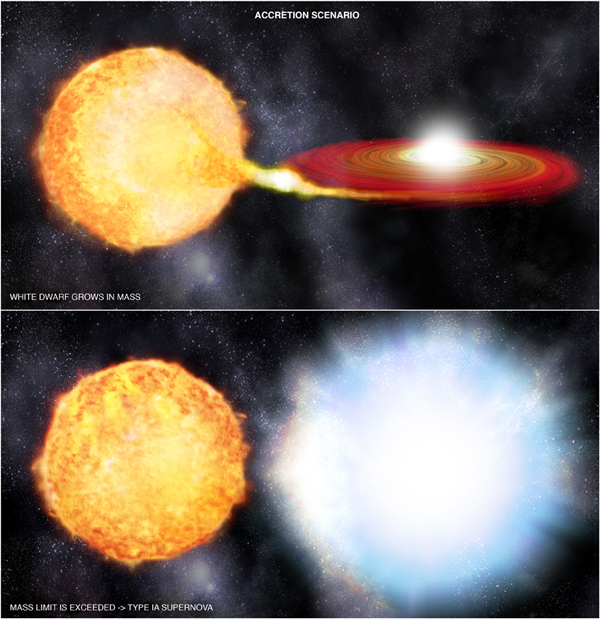
\includegraphics[width=0.3\textwidth]{figures/type_ia.jpg}}
                \put(60,0){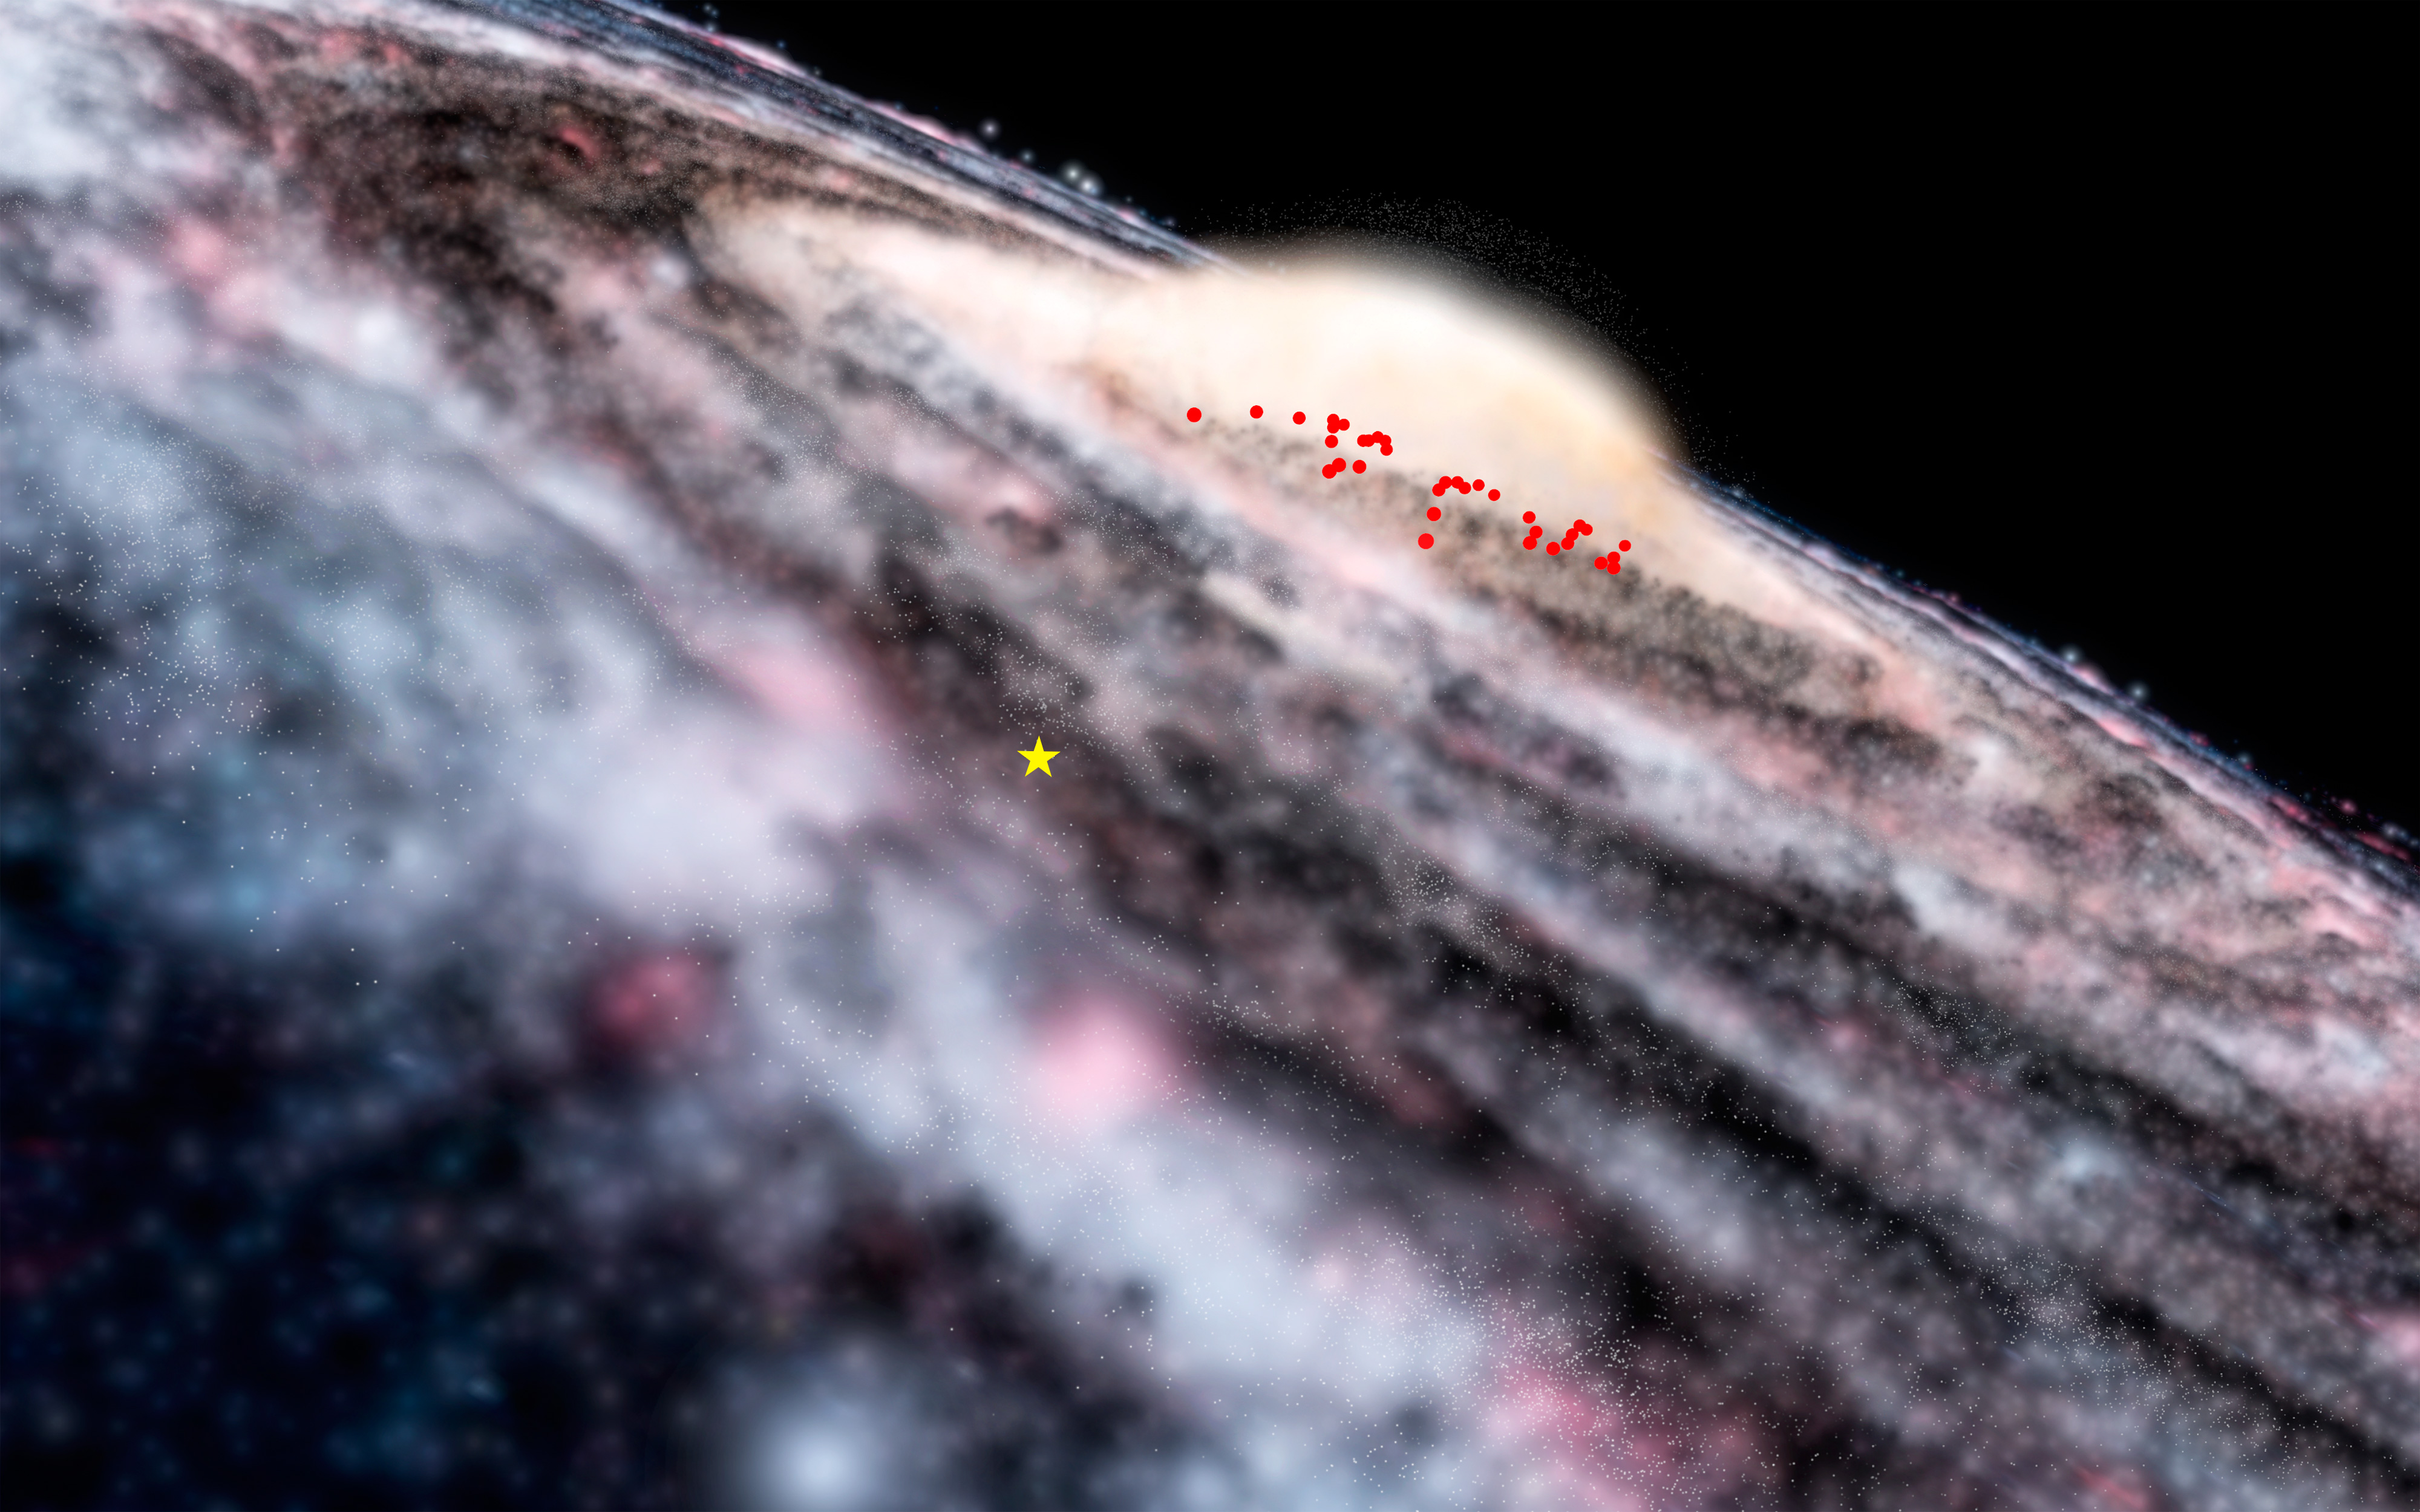
\includegraphics[width=0.4\textwidth]{figures/cepheid.jpg}}
                \put(70,25){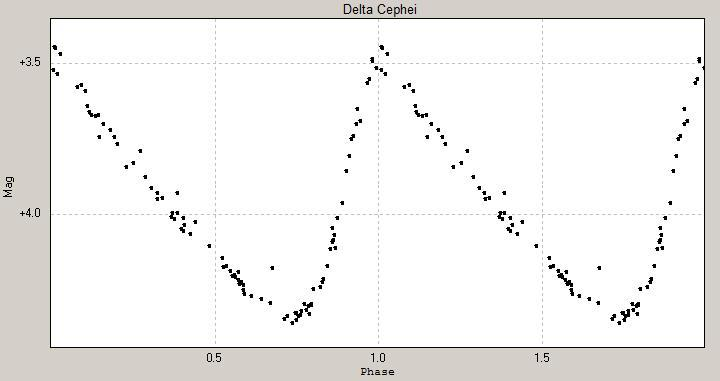
\includegraphics[width=0.3\textwidth]{figures/cepheid_curve.jpg}}
            \end{overpic}
        }
    \end{columns}
\end{frame}

\begin{frame}
    \frametitle{Standard Rulers}
    \begin{columns}
        \column{0.55\textwidth}
        \begin{itemize}
            \item<1-> Standard Rulers: Objects with known physical size.
\item<2-> CMB: Cosmic Microwave Background, fluctuations give a standard ruler at z$\sim$1100. \hfill \doi{10.1086/186504}
            \item<3-> BAO: Baryon Acoustic Oscillations, sound waves in early universe imprint a standard ruler on galaxy distribution. \hfill \arxiv{1201.2434}
            \item<4-> Strong lensing: Time delays between multiple images of a lensed object constrain distances. \hfill \doi{10.1093/mnras/128.4.307}
            \item<5-> Weak lensing: Distortion of galaxy shapes by intervening matter constrains the matter distribution.
        \end{itemize}
        \column{0.45\textwidth}
        \includegraphics<1>[width=\textwidth]{figures/rulers.jpg}
    \end{columns}
\end{frame}

\begin{frame}
    \frametitle{Standard Rulers}
    \framesubtitle{The cosmic microwave background}
    \begin{columns}
        \column{0.55\textwidth}
        \begin{itemize}
            \item<1-> CMB:  "Surface of last scattering" at $z\sim1100$.  Angular size of hot/cold spots gives a standard ruler. \hfill \doi{10.1086/186504}
            \item<2-> Temperature fluctuations: $\Delta T/T \sim 10^{-5}$.  \hfill \doi{10.1086/186504} 
            \item<2->  Polarization: E and B modes.  B-modes from primordial gravitational waves are a key target.
        \end{itemize}
        \column{0.45\textwidth}
        \includegraphics<1>[width=\textwidth]{figures/cmb.png}
        \includegraphics<2>[width=\textwidth]{figures/cmb_power_spectrum.jpg}%
    \end{columns}
\end{frame}

\begin{frame}
    \frametitle{Standard Rulers}
    \framesubtitle{Baryon Acoustic Oscillations}
    \begin{columns}
        \column{0.55\textwidth}
        \begin{itemize}
            \item<1-> BAO: Sound waves in the early Universe imprint a characteristic scale on the distribution of baryons (and galaxies). \hfill \arxiv{1201.2434}
            \item<2-> SDSS: Sloan Digital Sky Survey, one of the first surveys to measure BAO. \hfill \oldarxiv{astro-ph/0501171}
            \item<3-> DESI: Dark Energy Spectroscopic Instrument, current best BAO measurements. \hfill \arxiv{2404.03001}
        \end{itemize}
        \column{0.45\textwidth}
        \includegraphics<2>[width=\textwidth]{figures/desi_galaxies.png}
        \includegraphics<3>[width=\textwidth]{figures/desi_bao.jpg}%
    \end{columns}
\end{frame}

\begin{frame}
    \frametitle{Standard Rulers}
    \framesubtitle{Strong Lensing}
    \begin{columns}
        \column{0.55\textwidth}
        \begin{itemize}
            \item<1-> Strong Lensing: Light from a distant object is bent by the gravity of a massive foreground object (e.g., a galaxy or galaxy cluster). \hfill \doi{10.1093/mnras/128.4.307}
            \item<2-> Time Delays: Differences in path lengths of multiple images lead to time delays, which can be used to measure distances. \hfill \arxiv{2210.15794}
        \end{itemize}
        \column{0.45\textwidth}
        \includegraphics<1>[width=\textwidth]{figures/time_delay.jpg}
        \includegraphics<2>[width=\textwidth]{figures/time_delay_curve.png}%
    \end{columns}
\end{frame}

\begin{frame}
    \frametitle{Standard Rulers}
    \framesubtitle{Weak Lensing}
    \begin{columns}
        \column{0.55\textwidth}
        \begin{itemize}
            \item<1-> Weak Lensing:  Small distortions in the shapes of background galaxies caused by the gravitational lensing of intervening matter.
            \item<1-> Surveys like DES, KiDS, and HSC have used weak lensing to map the distribution of dark matter. \hfill \arxiv{1610.04606}\arxiv{1910.05336}
        \end{itemize}
        \column{0.45\textwidth}
        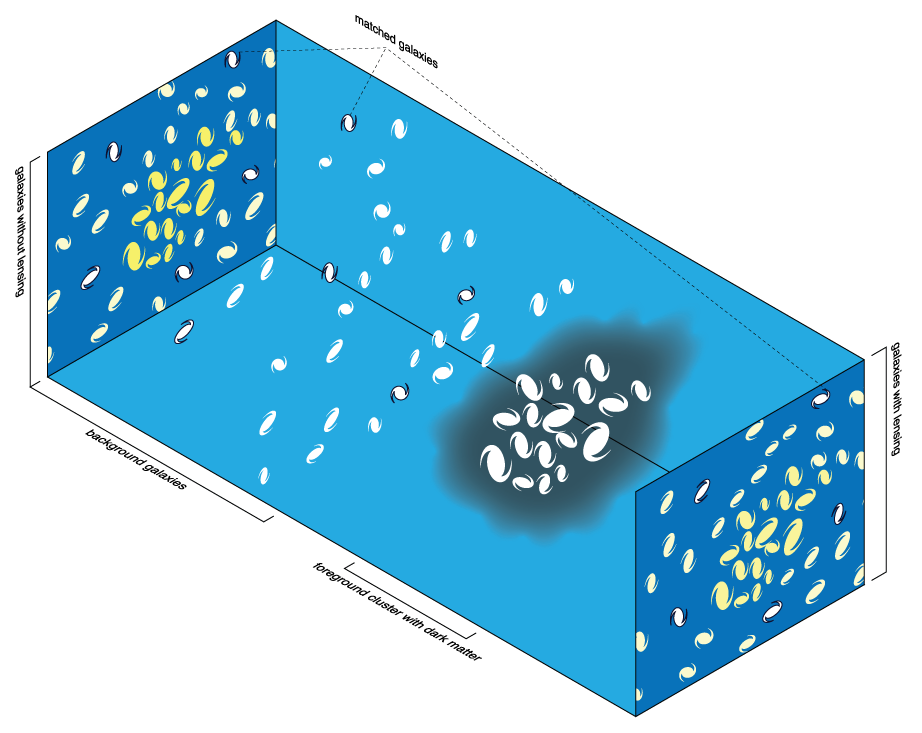
\includegraphics[width=\textwidth]{figures/weak_lensing.png}
    \end{columns}
\end{frame}

\begin{frame}
    \frametitle{Standard Sirens}
    \begin{columns}
        \column{0.5\textwidth}
        \begin{itemize}
            \item<1-> Standard Sirens: Gravitational wave sources with known intrinsic "loudness". \hfill \doi{10.1038/323310a0} \oldarxiv{astro-ph/0504616}
            \item<2-> Bright sirens: GW events with an electromagnetic counterpart, allowing redshift measurement. \hfill \arxiv{1710.05835}
            \item<3-> Dark sirens: GW events without an electromagnetic counterpart; statistical redshift information is used. \hfill \arxiv{1901.01540}
            \item<4-> Spectral sirens: Redshift is inferred statistically from the mass distribution of merging black holes. \hfill \arxiv{1908.09084}
        \end{itemize}
        
        \column{0.5\textwidth}
        \includegraphics<1>[height=0.33\textwidth]{figures/gw.jpg}%
        \includegraphics<2>[height=0.33\textwidth]{figures/gw_local.jpg}
        \includegraphics<3->[width=\textwidth]{figures/posterior_O3_dr9beta_170817.png} % 2111.06445
        
    \end{columns}
\end{frame}

\begin{frame}
    \frametitle{Standard Clocks}
    \begin{columns}
        \column{0.5\textwidth}
        \begin{itemize}
            \item<1-> Standard Clocks: Objects or phenomena whose time evolution can be used to measure time or distances.
            \item<2-> Cosmic Chronometers: Passively evolving galaxies whose age can be measured, giving $dH/dz$. \hfill \oldarxiv{astro-ph/0106145}
            \item<3-> Pulsar timing arrays: Variations in the arrival times of pulsar signals can be used to detect gravitational waves and measure distances.
        \end{itemize}
        \column{0.5\textwidth}
        %\includegraphics[width=\textwidth]{figures/clocks.jpg}
        \includegraphics<1>[width=\textwidth]{figures/timers.jpg}
        \includegraphics<2>[width=\textwidth]{figures/cosmic_chronometers.png}
        \includegraphics<3>[width=\textwidth]{figures/pulsar_timing_array.jpg}
    \end{columns}
\end{frame}
 
\begin{frame}
    \frametitle{The Hubble tension}
    \begin{columns}
        \column{0.5\textwidth}
        \begin{itemize}
            \item CMB: $H_0=67.4\pm0.5$ km/s/Mpc. \hfill \arxiv{1807.06209}
            \item S$H_0$ES: $H_0=73.2\pm1.3$ km/s/Mpc. \hfill \arxiv{2112.04510}
            \item Exciting if not measurement error
                \begin{itemize}
                    \item People trust the CMB measurement, but perhaps not the $\Lambda$CDM model assumptions.
                    \item Measurements of $H_0$ from supernovae are notoriously challenging (crowding, dust, metallicity, etc.)
                \end{itemize}
            \item As of 2024, Hubble three ways (Cepheids, TRGB, JAGB) show some convergence:
                \begin{description}
                    \item [CCHP (Freedman)] $H_0 = (72.0, 69.8, 67.96)\pm1.8$ km/s/Mpc
                    \item [SH0ES (Riess)] $H_0 = (73.4, 72.1, 72.2)\pm2.2$ km/s/Mpc
                \end{description}                                      
                \hfill\arxiv{2408.06153}\arxiv{2408.11770}
        \end{itemize}
        \column{0.5\textwidth}
        \includegraphics<1>[width=\textwidth]{figures/H0_1.jpg}%
        \includegraphics<2>[width=\textwidth]{figures/H0_2.jpg}%
        \includegraphics<3>[width=\textwidth]{figures/H0_3.png}%
        \includegraphics<4>[width=\textwidth]{figures/H0_4.png}%
        \only<5>{
            \begin{overpic}[height=0.9\textheight]{figures/hH0whisker_Chapter2_SameRowColor4_SN_P15.pdf}
                \put(18,4){\tiny\arxiv{2103.01183}}
            \end{overpic}
        }
    \end{columns}
\end{frame}

\begin{frame}
    \frametitle{The $S_8$ tension}
    \framesubtitle{aka $\sigma_8$/weak lensing tension}
    \begin{columns}
        \column{0.52\textwidth}
        \begin{itemize}
            \item $S_8$ quantifies the amplitude of matter fluctuations on large scales.
            \item $S_8=\sigma_8(\Omega_m/0.3)^{0.5}$.
            \item CMB: $S_8 \approx 0.834$. \hfill \arxiv{1807.06209}
            \item Weak lensing:  $S_8 \approx 0.76$. \hfill \arxiv{1610.04606}\arxiv{1910.05336}
            \item Tension at the $2-3\sigma$ level.
            \item Possible systematics in weak lensing or new physics?
        \end{itemize}
        \column{0.48\textwidth}
         \includegraphics<1>[width=\textwidth]{figures/K+Dcontour_sig8om.pdf}%
        \includegraphics<2>[width=\textwidth]{figures/K+Dcontour.pdf}%
        \only<3>{%
        \begin{overpic}[width=\textwidth]{figures/s8_tension.pdf}
            \put(0,0){\arxiv{2402.08458}}
        \end{overpic}}
    \end{columns}
    \hfill\arxiv{2305.17173}
\end{frame}

\begin{frame}
    \frametitle{Other Tensions and Anomalies}
    \begin{columns}
        \column{0.5\textwidth}
        \begin{itemize}
            \item $A_{\rm lens}$ anomaly: CMB lensing amplitude higher than expected. \hfill \arxiv{1807.06209}
            \item Non-zero curvature: Some data hints at a closed universe. \hfill \arxiv{1902.04029}
            \item CMB anisotropic anomalies:  Large-scale features that challenge statistical isotropy. \hfill \arxiv{1510.07929}
            \item BBN anomalies: Discrepancies in light element abundances. \hfill \arxiv{1912.01132}
        \end{itemize}
        \column{0.5\textwidth}
        \begin{overpic}[width=\textwidth]{figures/omegak_H0.pdf} 
            \put(0,0){\tiny\arxiv{1908.09139}}
        \end{overpic}
        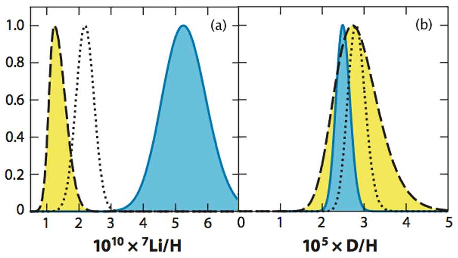
\includegraphics[width=\textwidth]{figures/lithium.pdf}
    \end{columns}
\end{frame}

\begin{frame}
    \frametitle{Cosmology in 2024}
    \begin{columns}
        \column{0.5\textwidth}
        \begin{itemize}
            \item 2024 was a big year for cosmology, with new data releases from multiple surveys:
                \begin{description}
                    \item[Jan] DESY5 SNe:  Improved supernova measurements from the Dark Energy Survey. \hfill \arxiv{2401.02929}
                    \item[Feb] eROSITA: First all-sky survey results from the extended ROentgen Survey with an Imaging Telescope Array. \hfill \arxiv{2402.08458}
                    \item[Mar] DESI:  First year cosmology results from the Dark Energy Spectroscopic Instrument. \hfill \arxiv{2404.03002}
                \end{description}
                \item These releases provide new insights into cosmic tensions, but also highlight the need for further investigation.
        \end{itemize}
        \column{0.5\textwidth}
        \includegraphics<1>[width=\textwidth]{figures/HD_5yr_KeyPaper.pdf}
        \includegraphics<2>[height=0.42\textwidth]{figures/LCDM_paper.pdf}%
        \includegraphics<3>[height=0.42\textwidth]{figures/w0wa_paper_wZoom.pdf}
    \end{columns}
\end{frame}

\begin{frame}
    \frametitle{eROSITA}
    \begin{columns}
        \column{0.5\textwidth}
        \begin{itemize}
            \item eROSITA performed the first all-sky survey in X-rays since ROSAT.
            \item Detected $\sim$12,000 galaxy clusters, providing a powerful new dataset for cosmology.
            \item Results broadly consistent with $\Lambda$CDM, but with some hints of tension in $\sigma_8$. \hfill \arxiv{2402.08458}
        \end{itemize}
        \column{0.5\textwidth}
        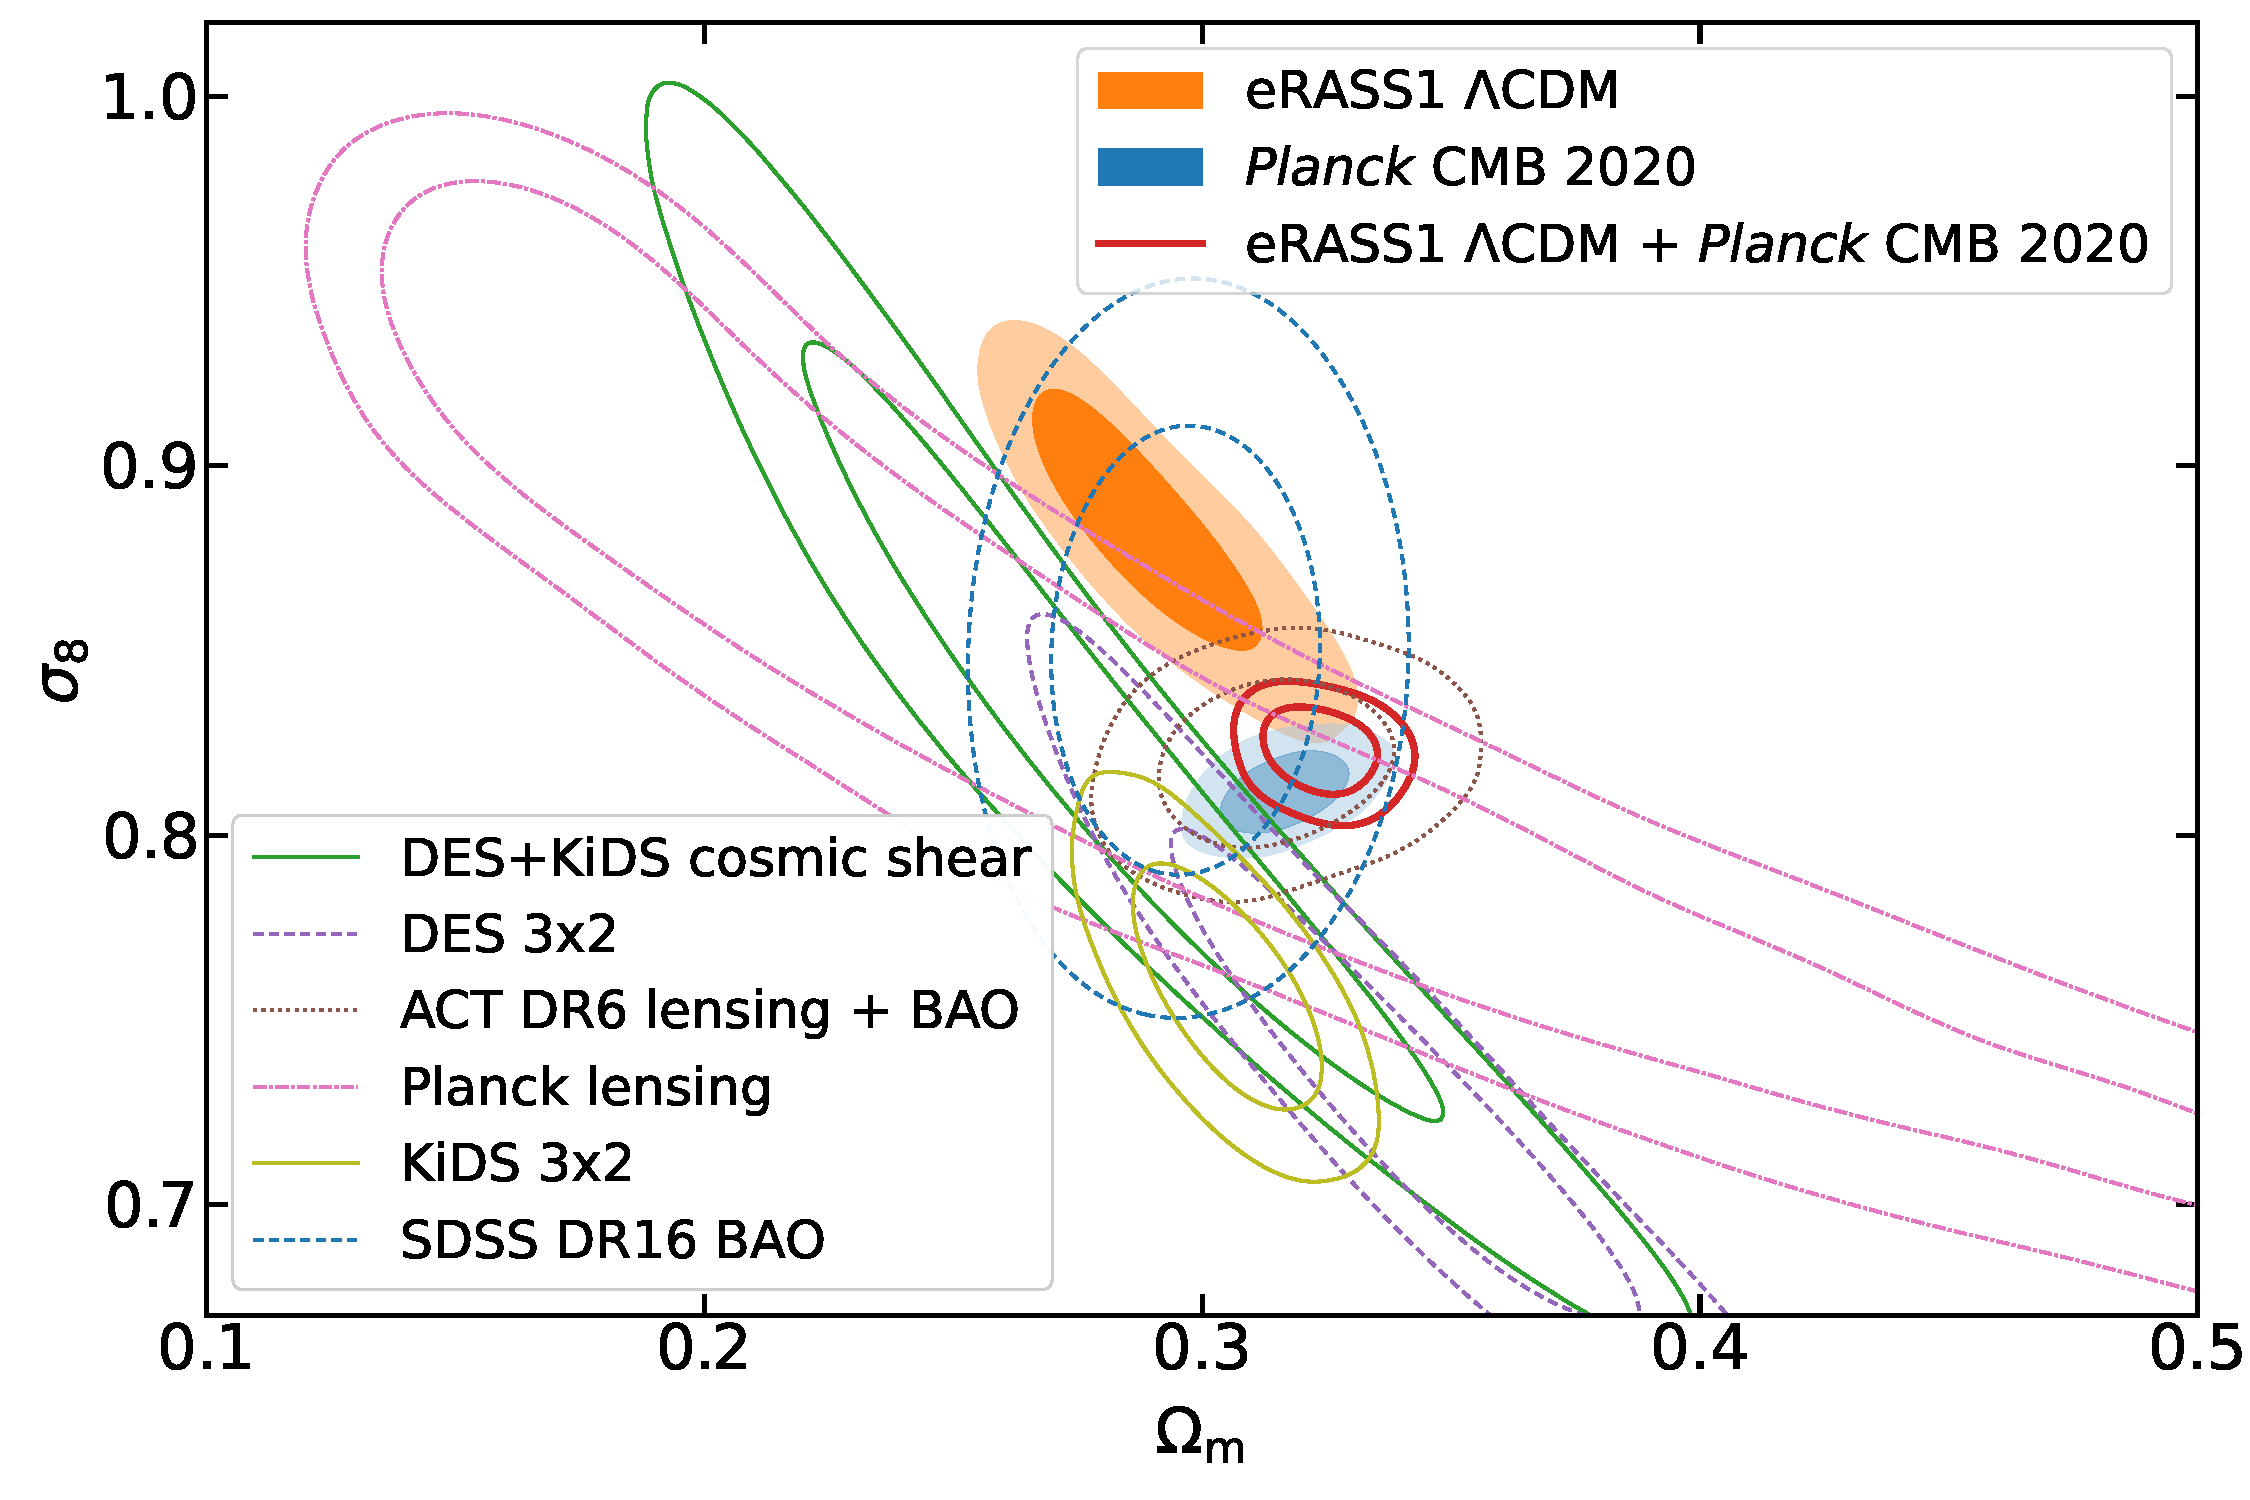
\includegraphics[width=\textwidth]{figures/eROSITA.pdf}
    \end{columns}
\end{frame}

\begin{frame}
    \frametitle{DESI}
    \begin{columns}
        \column{0.5\textwidth}
        \begin{itemize}
            \item DESI is mapping millions of galaxies and quasars to measure BAO and redshift-space distortions.
            \item First year cosmology results strengthen evidence for dark energy, but do not resolve the $H_0$ tension. \hfill \arxiv{2404.03002}
            \item Full BAO and BBN analysis yields $H_0 = 68.53 \pm 0.80$ km/s/Mpc (independent of CMB). \hfill \arxiv{2404.03000}
        \end{itemize}
        \column{0.5\textwidth}
        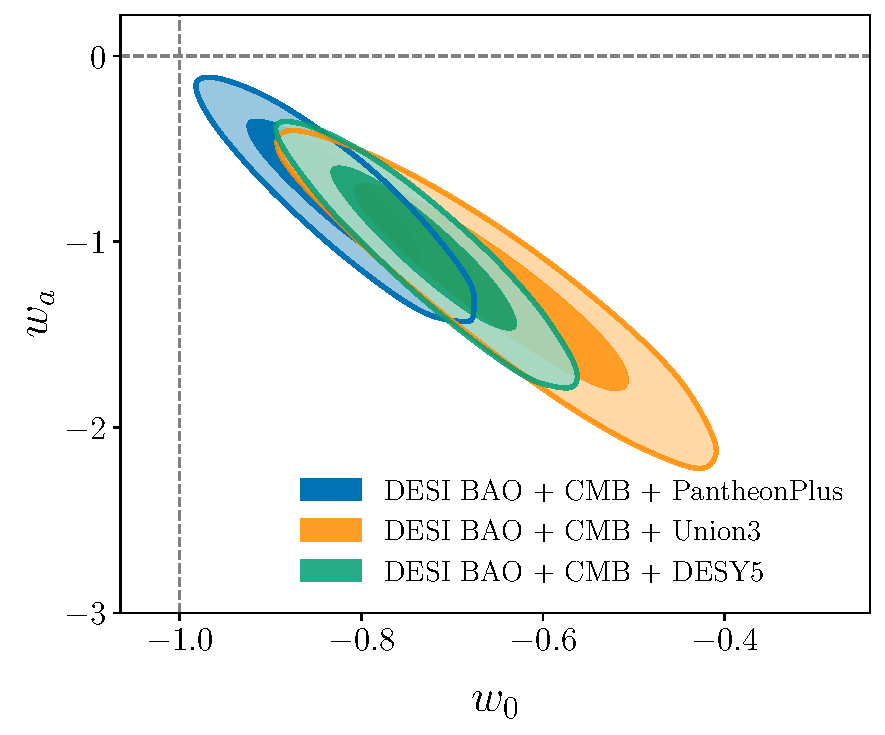
\includegraphics[width=\textwidth]{figures/w0wa_DESI-Planck-SN-95lim.pdf}
    \end{columns}
\end{frame}

\begin{frame}
    \frametitle{What to watch out for}
    \begin{columns}
        \column{0.33\textwidth}
        \begin{itemize}
            \item In 2025:
                \begin{itemize}
                    \item DESI: Year 3 BAO results with increased precision.
                    \item DES/Euclid: Improved weak lensing measurements with larger sky coverage.
                    \item eROSITA: Further analysis of X-ray cluster data, including mass calibration.
                    \item ACT: Final data release with improved CMB polarization measurements.
                    \item LVK: Continued gravitational wave observations, potentially increasing the number of standard sirens.
                \end{itemize}
            \item Next 5 years:
                \begin{itemize}
                    \item Simons Observatory: High-precision CMB observations, targeting primordial B-modes.
                    \item Rubin: First light and early strong lensing discoveries.
                    \item Roman: Hubble 3.0 with improved Cepheid measurements.
                    \item IPTA: Improved pulsar timing array data, constraining the stochastic gravitational wave background.
                \end{itemize}
            \item Next 10-20 years:
                \begin{itemize}
                    \item LISA/Einstein Telescope: Next-generation gravitational wave observatories, probing the early Universe.
                    \item SKA: Large FRB surveys, constraining cosmological parameters and the intergalactic medium.
                    \item LiteBird: Space-based CMB polarization measurements, targeting primordial B-modes.
                    \item ATHENA: High-resolution X-ray observations of galaxy clusters, improving mass calibration.
                \end{itemize}
        \end{itemize}
        \column{0.67\textwidth}
       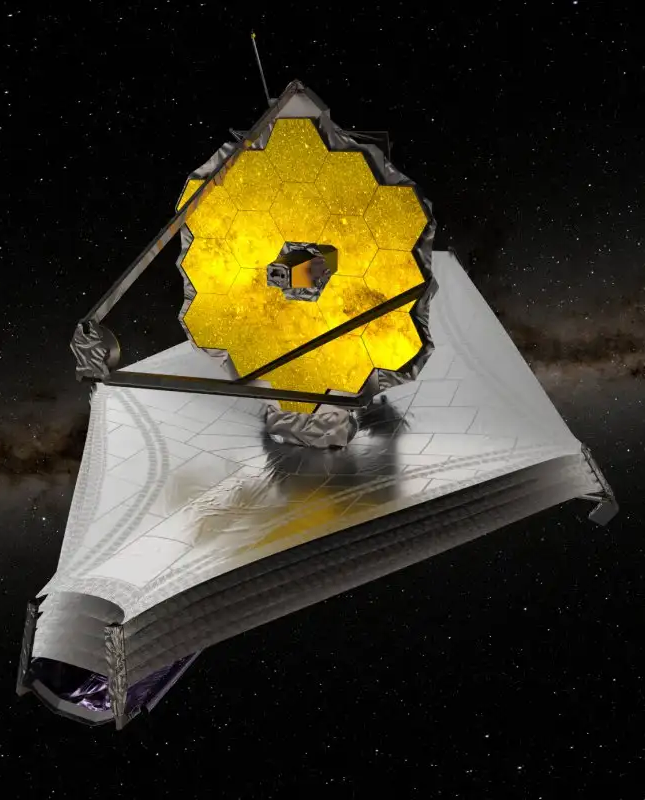
\includegraphics[height=0.145\textwidth]{figures/telescopes/jwst.png}%
        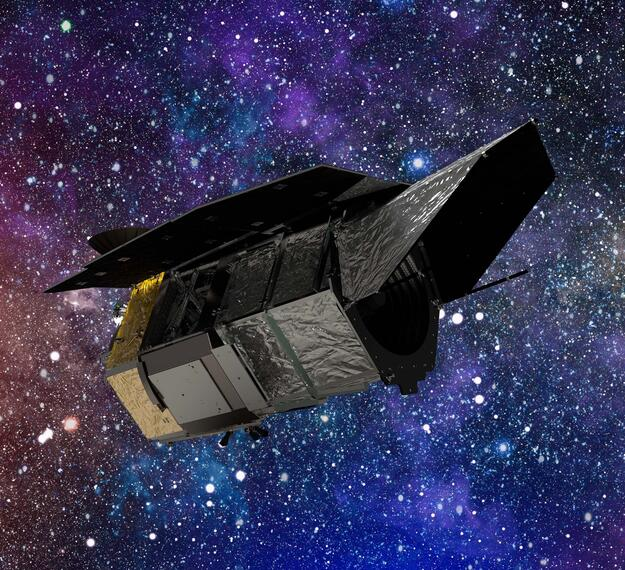
\includegraphics[height=0.145\textwidth]{figures/telescopes/roman.jpg}%
        \includegraphics[height=0.145\textwidth]{figures/telescopes/euclid.jpeg}%
        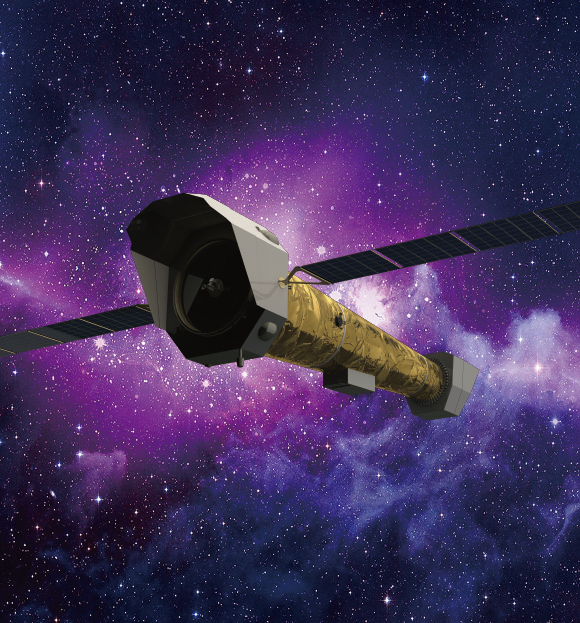
\includegraphics[height=0.145\textwidth]{figures/telescopes/athena.jpg}%
        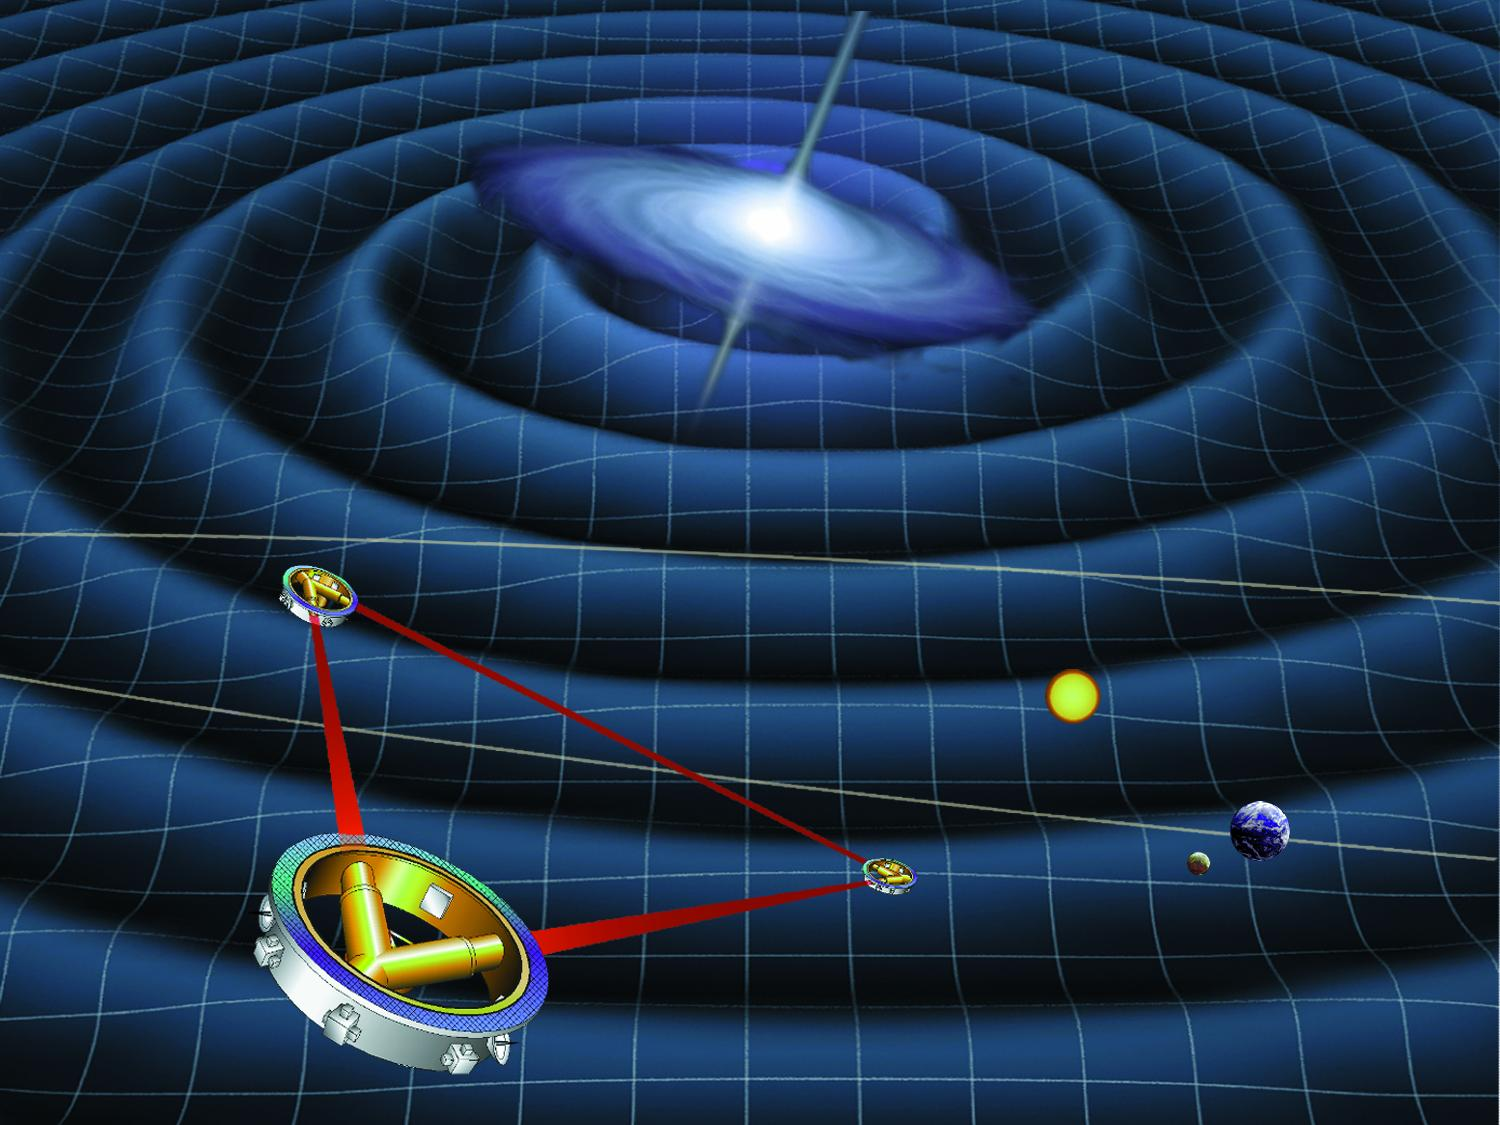
\includegraphics[height=0.145\textwidth]{figures/telescopes/lisa.jpg}%
        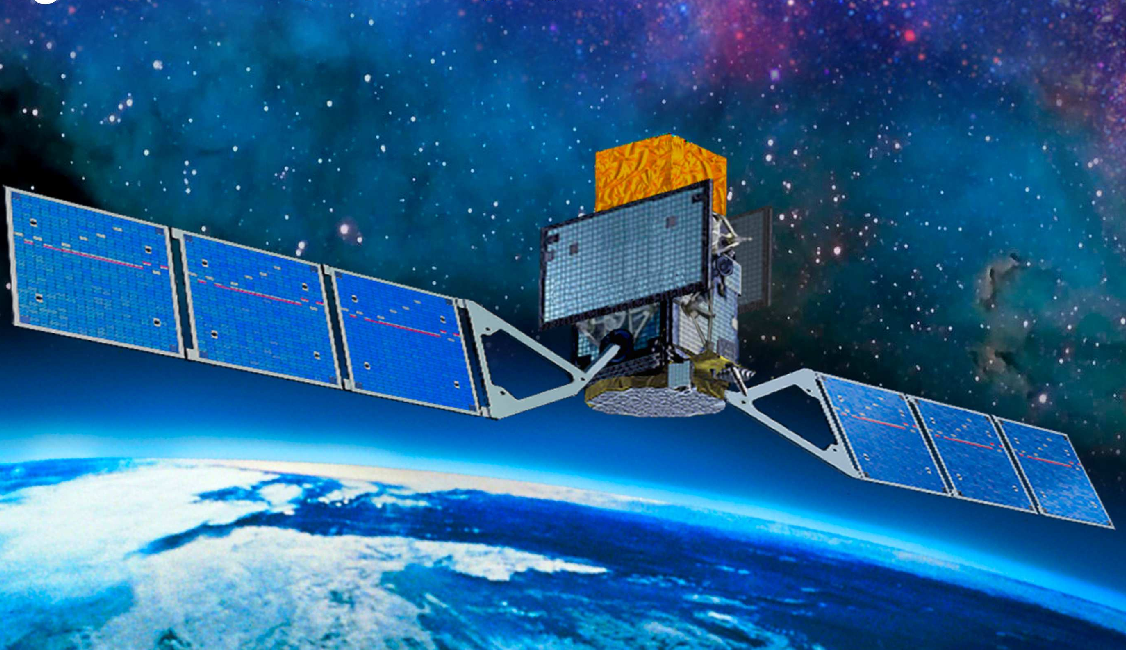
\includegraphics[height=0.145\textwidth]{figures/telescopes/e-ASTROGAM.pdf}%
        \vspace{-1pt}
        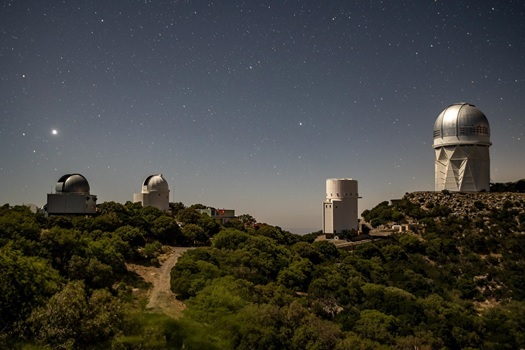
\includegraphics[height=0.15183\textwidth]{figures/telescopes/desi.jpg}%
        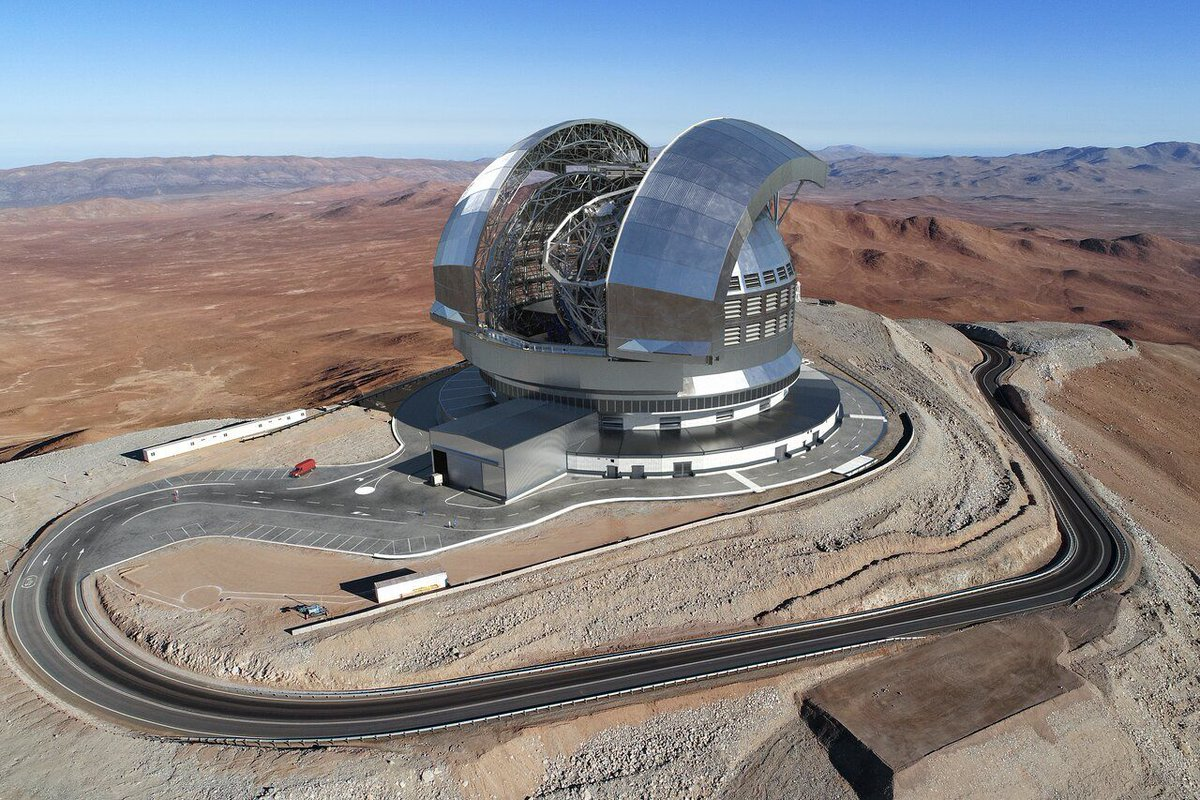
\includegraphics[height=0.15183\textwidth]{figures/telescopes/eelt.jpg}%
        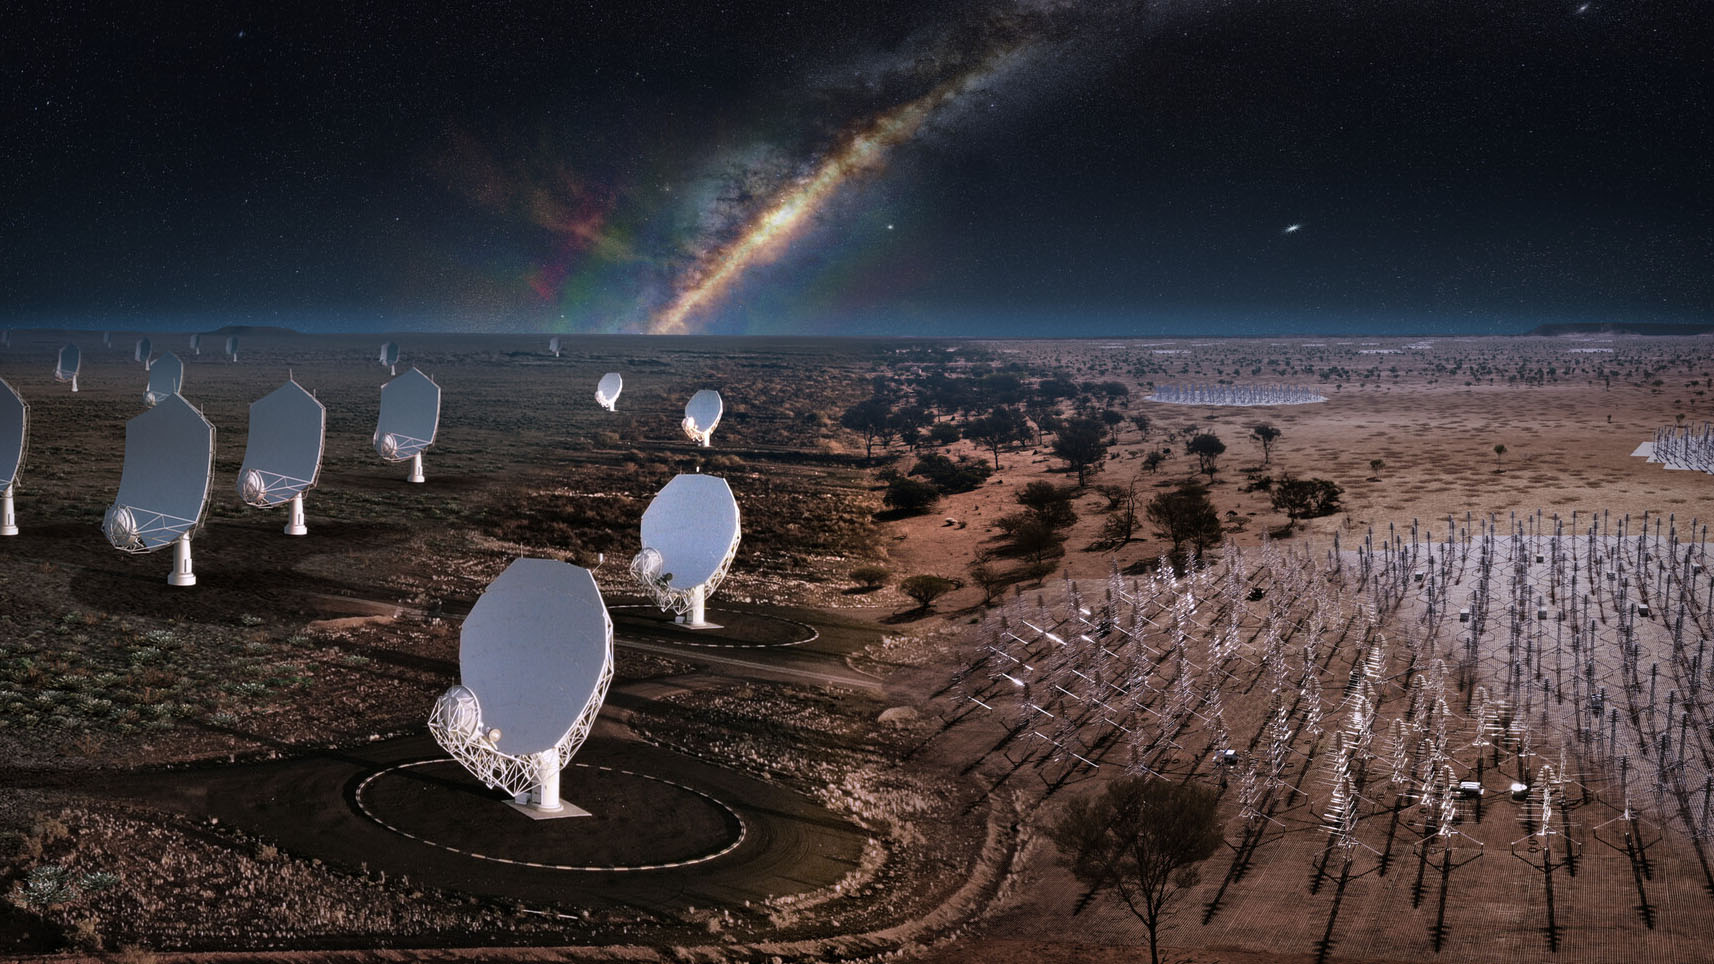
\includegraphics[height=0.15183\textwidth]{figures/telescopes/ska.jpg}%
        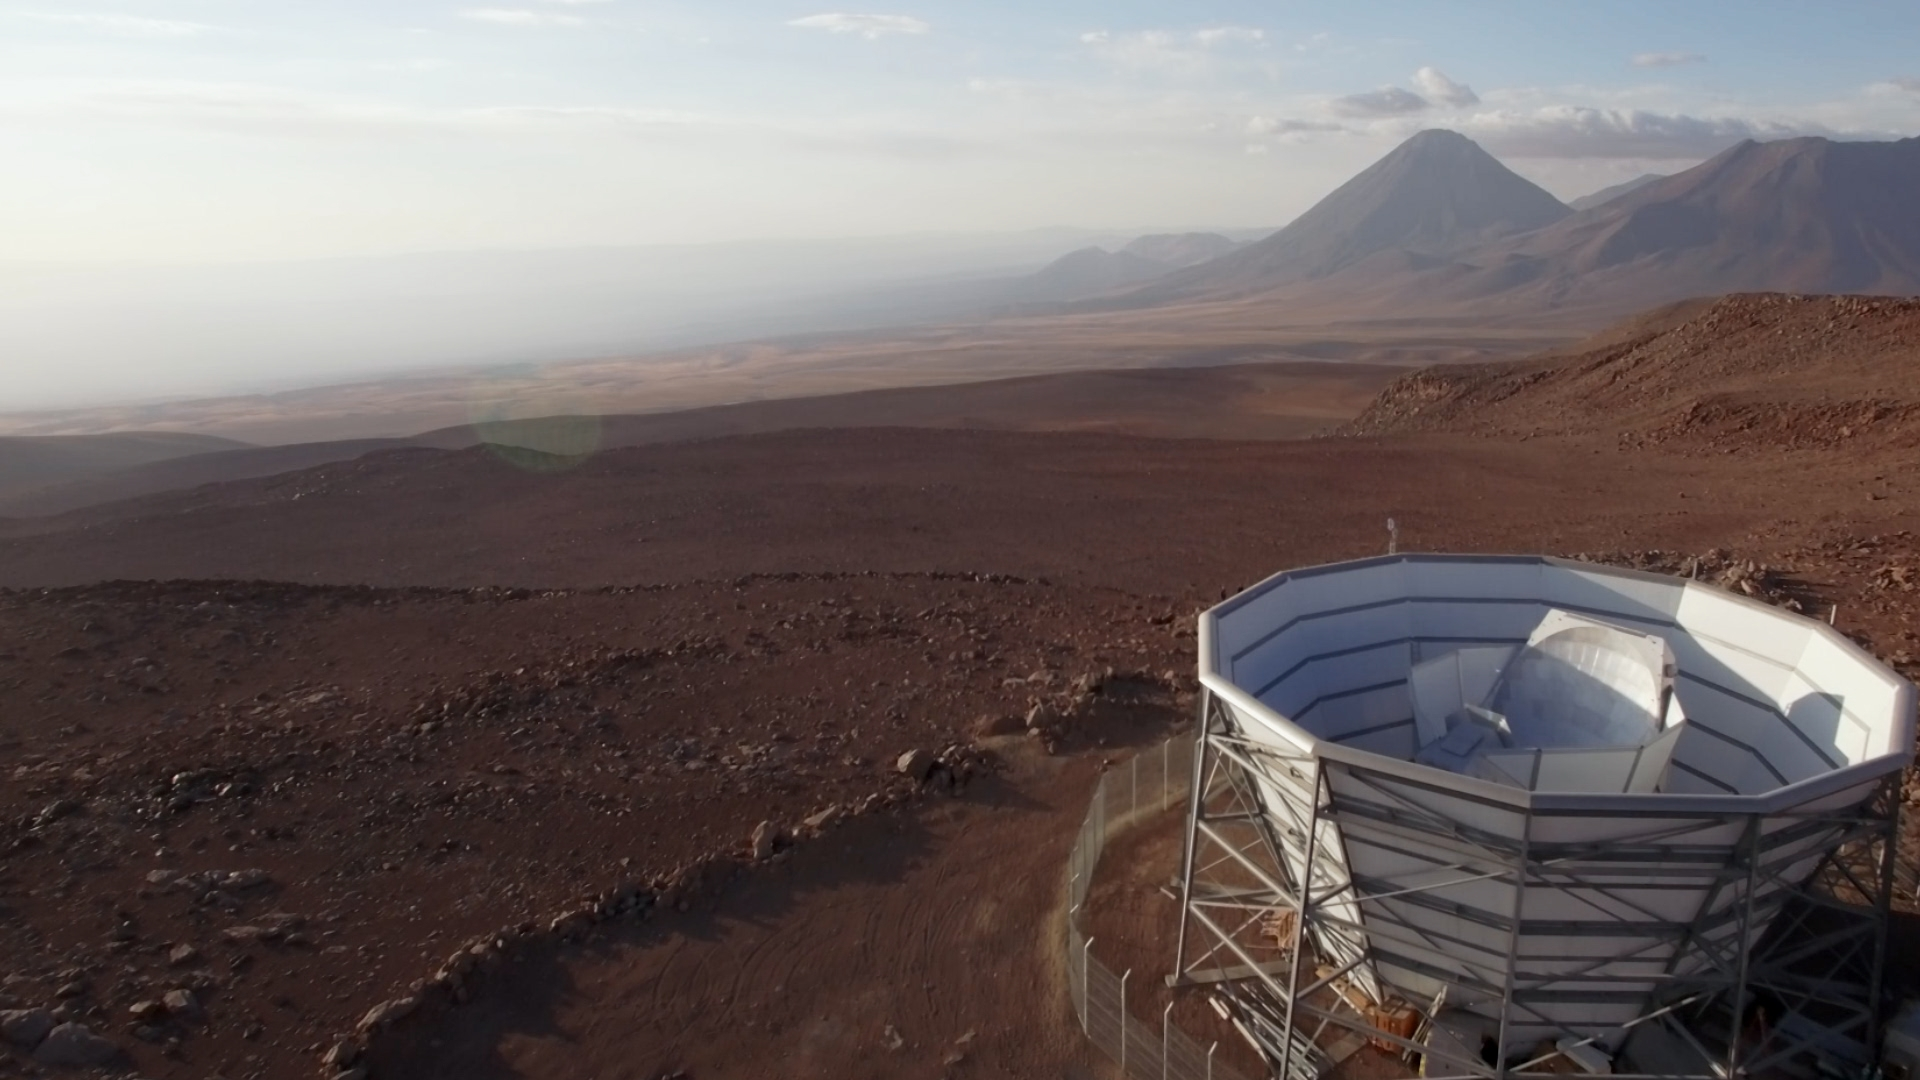
\includegraphics[height=0.15183\textwidth]{figures/telescopes/SO.jpg}%
        \vspace{-1pt}
        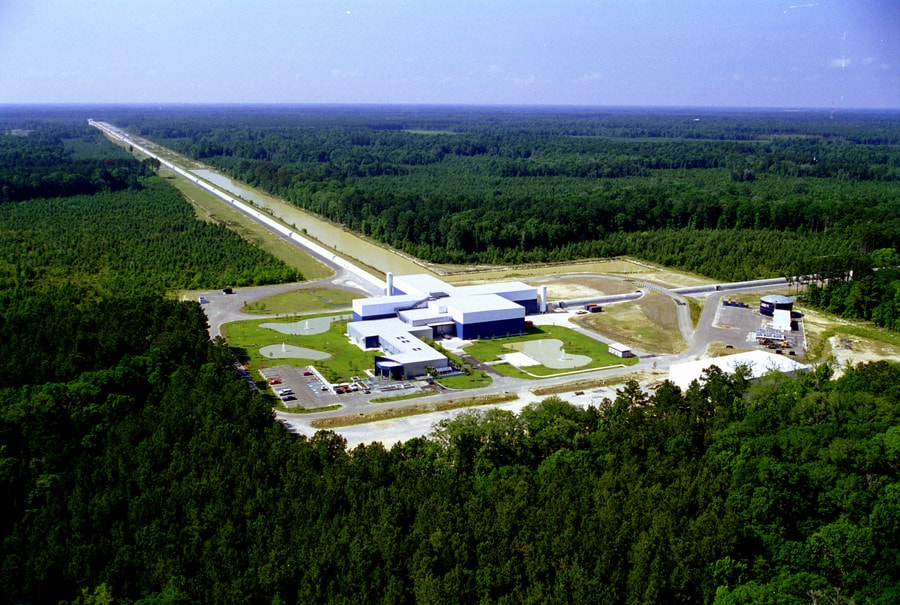
\includegraphics[height=0.18428\textwidth]{figures/telescopes/ligo.jpg}%
        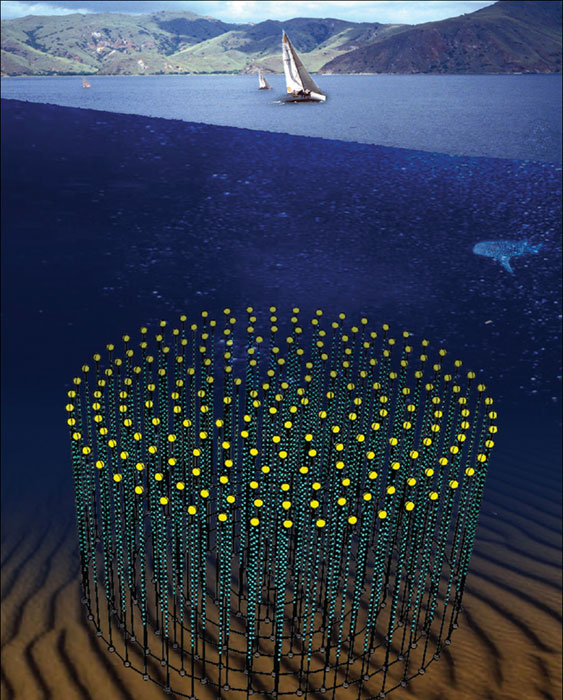
\includegraphics[height=0.18428\textwidth]{figures/telescopes/km3n.jpg}%
        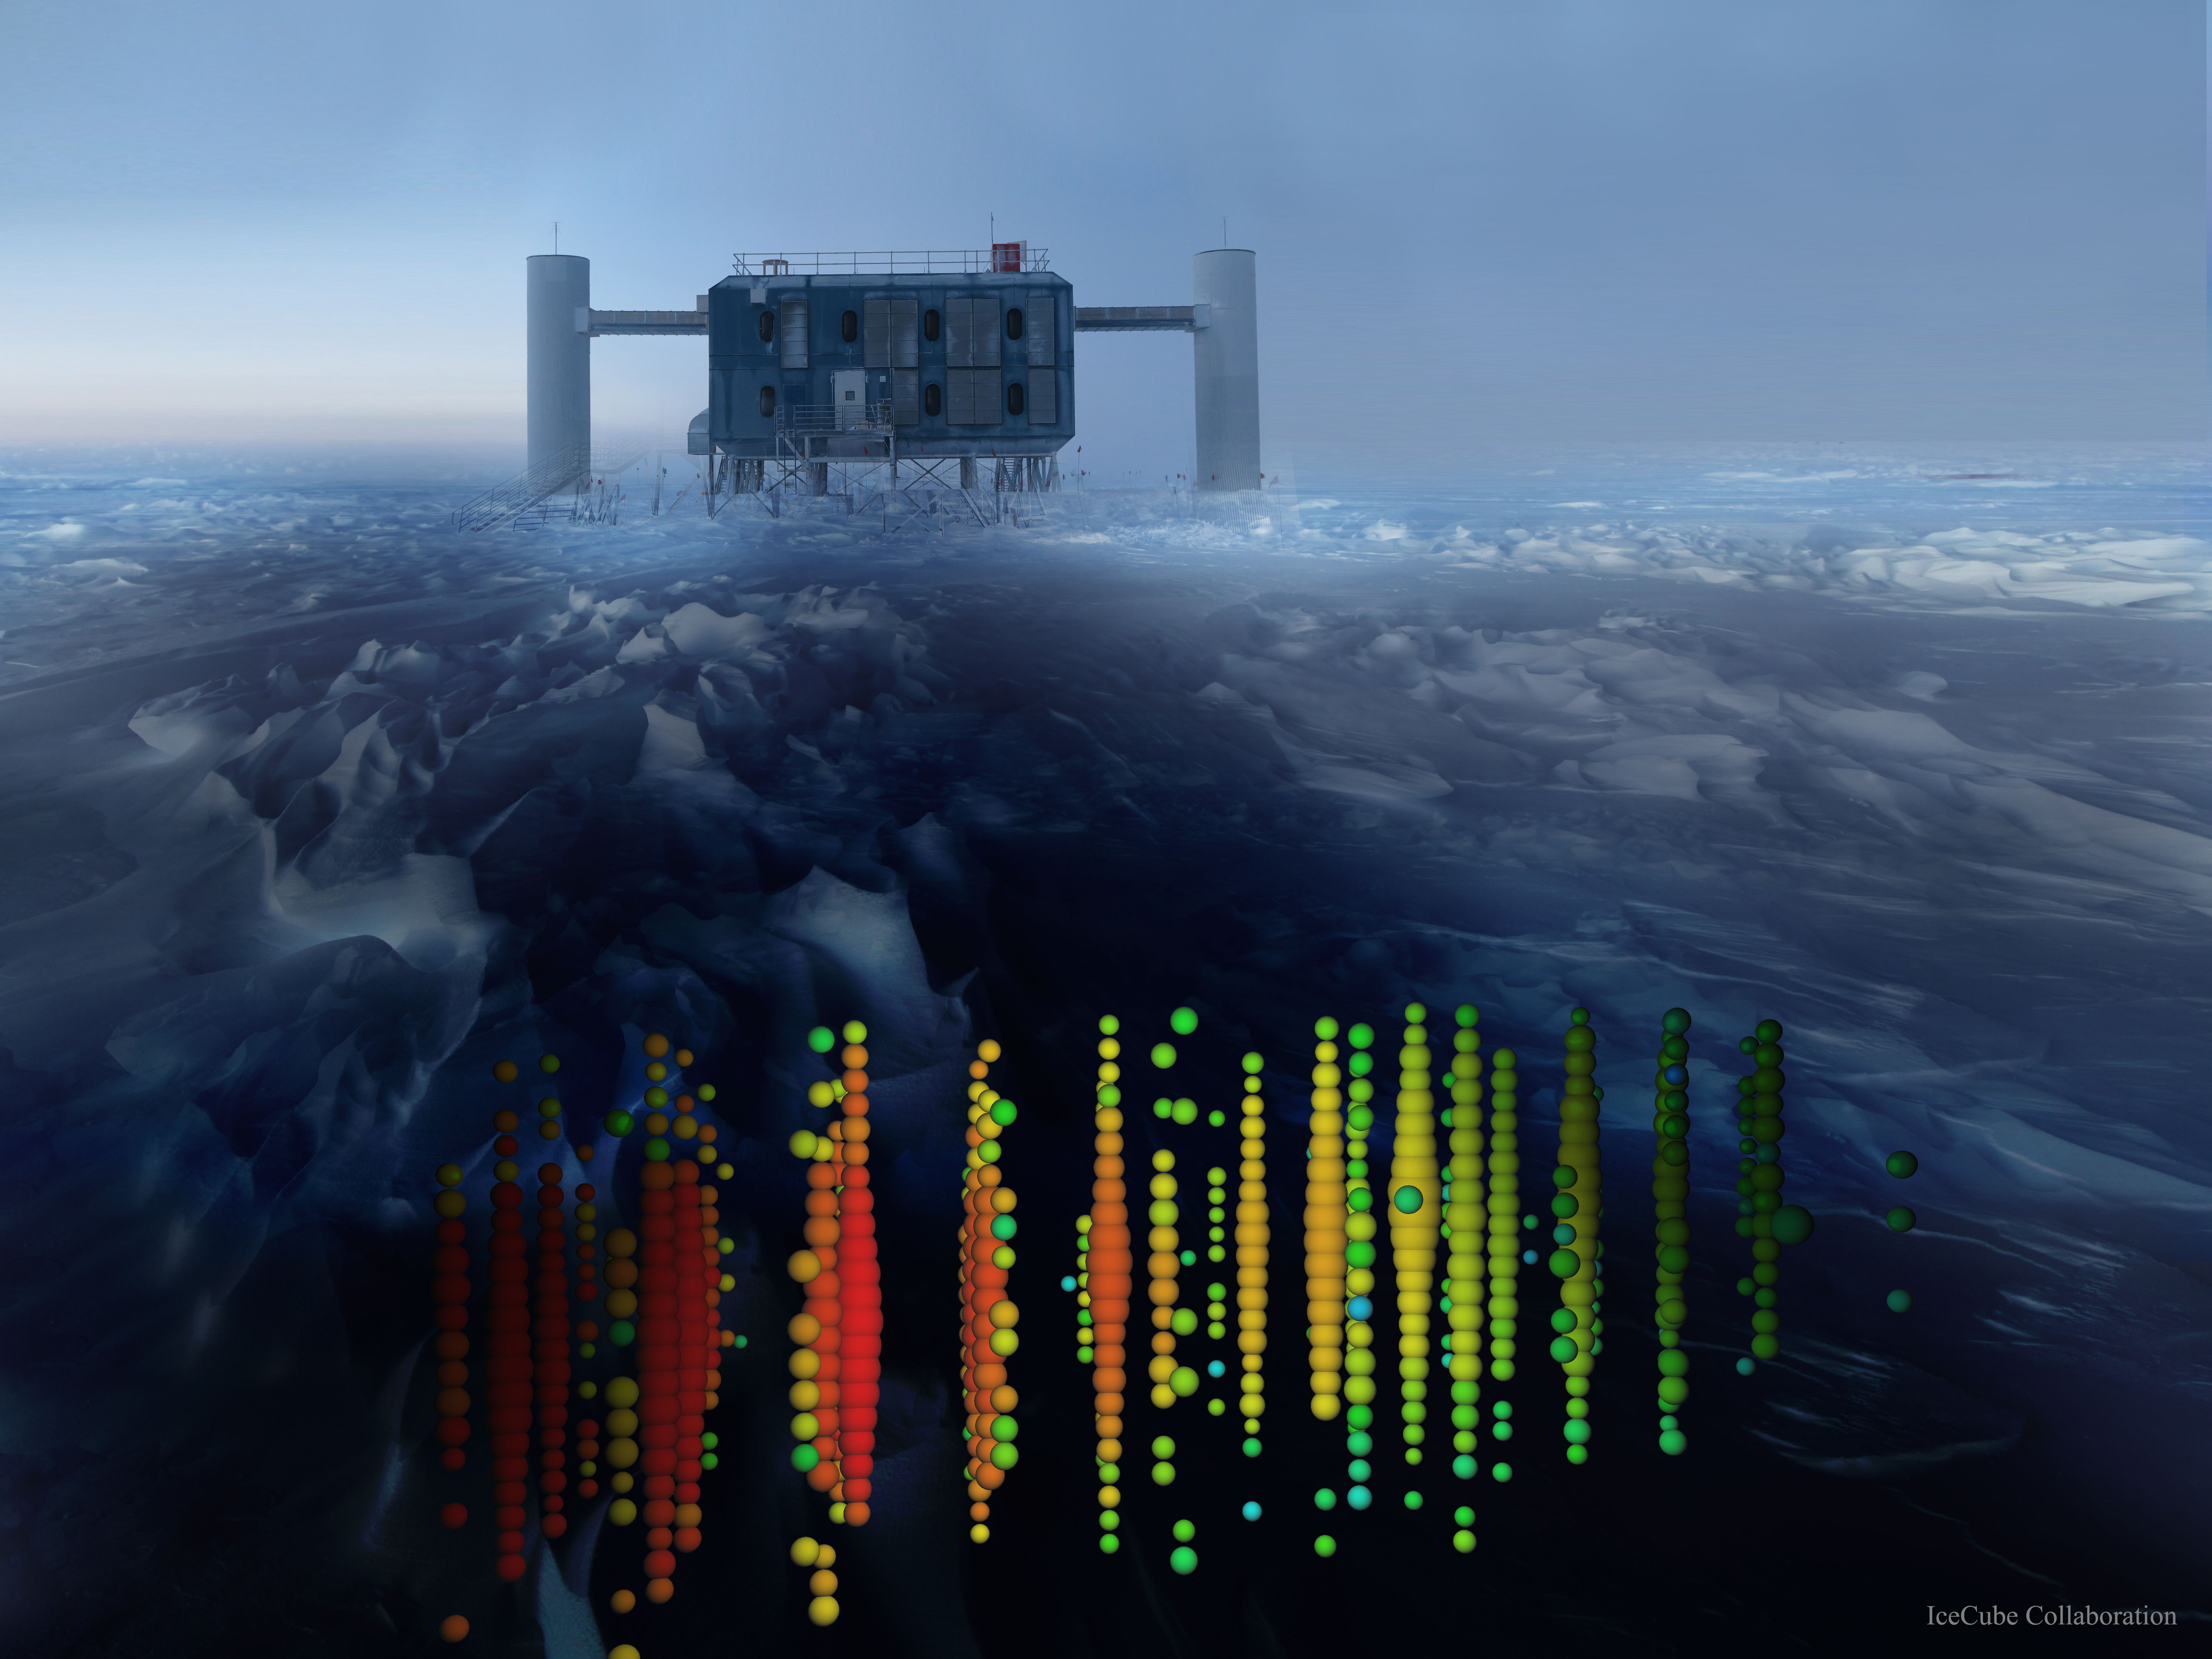
\includegraphics[height=0.18428\textwidth]{figures/telescopes/icecube.jpg}%
        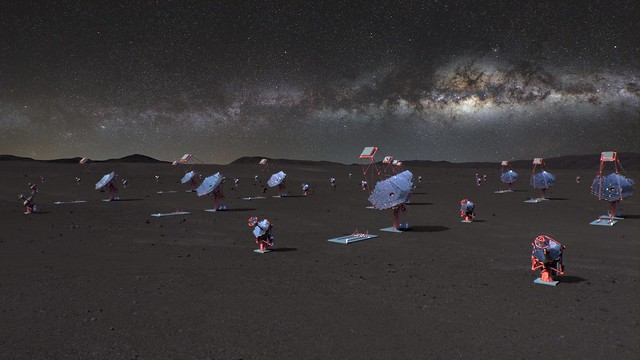
\includegraphics[height=0.18428\textwidth]{figures/telescopes/CTA.jpg}%
    \end{columns}
\end{frame}

\end{document}
